\documentclass[12pt]{article}
\usepackage{graphicx}
\usepackage{epstopdf}
\usepackage{booktabs}
\usepackage[table]{xcolor}
\usepackage{float}
\usepackage{caption}
\usepackage{hyperref}
\usepackage{adjustbox}
\usepackage{amsmath}
\usepackage{listings}
\usepackage[document]{ragged2e}
\usepackage{titling}
\usepackage{lipsum}

\author{Assignment 1 (Homography) \\ Vaishali Pal \\ 201407665}
\title{Computer Vision Assignment Report}
\date{\today}


\preauthor{\begin{flushright}\large} % makes author flush right
\postauthor{\end{flushright}}

\begin{document}
  \maketitle
  
\section{Introduction}
The purpose of this assignment is to estimate the homography matrix from images and be familiar with the applications of homography matrix. The algortithms used for this purpose are DLT and RANSAC.

\section{DLT with Manual Features}
DLT uses at least 4 image points to estimate the camera parameters. The points should not be collinear.

\subsection{Code} 
\begin{lstlisting}[language=matlab]
    imP2 = [658, 120, 1;
        784, 624, 1;
        402, 116, 1;
        1592, 164, 1;
        ];
    imP1 = [670, 120, 1;
        794, 622, 1;
        420, 118, 1;
        1592, 180, 1];
    

A = zeros(9,9);
    k = 1;
    for i = 1:4
        imPt = imP2(i, 1);
        A(k, 1:3) = -imP1(i,:);
        A(k,4:6) = zeros(1,3);
        A(k,7:9) = [imPt*imP1(i,1), imPt*imP1(i,2), imPt*imP1(i,3)];
        k = k + 1;

        imPt = imP2(i, 2);
        A(k,1:3) = zeros(1,3);
        A(k, 4:6) = -imP1(i,:);
        A(k,7:9) = [imPt*imP1(i,1), imPt*imP1(i,2), imPt*imP1(i,3)];
        k = k + 1;
    end

    [U, S, V] = svd(A);
    singV = diag(S);
    [~, indx] = sort(singV);
    p = V(:, indx(1));
    p = reshape(p, [3,3])';
    p = p/p(3,3);
    estimatedImg = p*imP1';
    imgEst = (estimatedImg ./ repmat(estimatedImg(3,:),3,1))';
    H = p(:,1:3);
    invH = inv(H);
    [invR, invK] = qr(invH);
    R = invR'
    K = inv(invK)
    C = invH*p(:,3)
    
  figure;
  imshow(I2);
  hold on;
  plot(imP2(:,1), imP2(:,2), 'r*', 'LineWidth',3);
  plot(imgEst(:,1), imgEst(:,2), 'bo', 'LineWidth',2);   
\end{lstlisting}

\subsection{Input}
The input to DLT are 4 image points from one of the images and the correspondinf points in the other image. For this experiment, 4 image points from each image have been chosen.

\begin{figure}[h]
\centering
\begin{minipage}{0.6\textwidth}
\centering
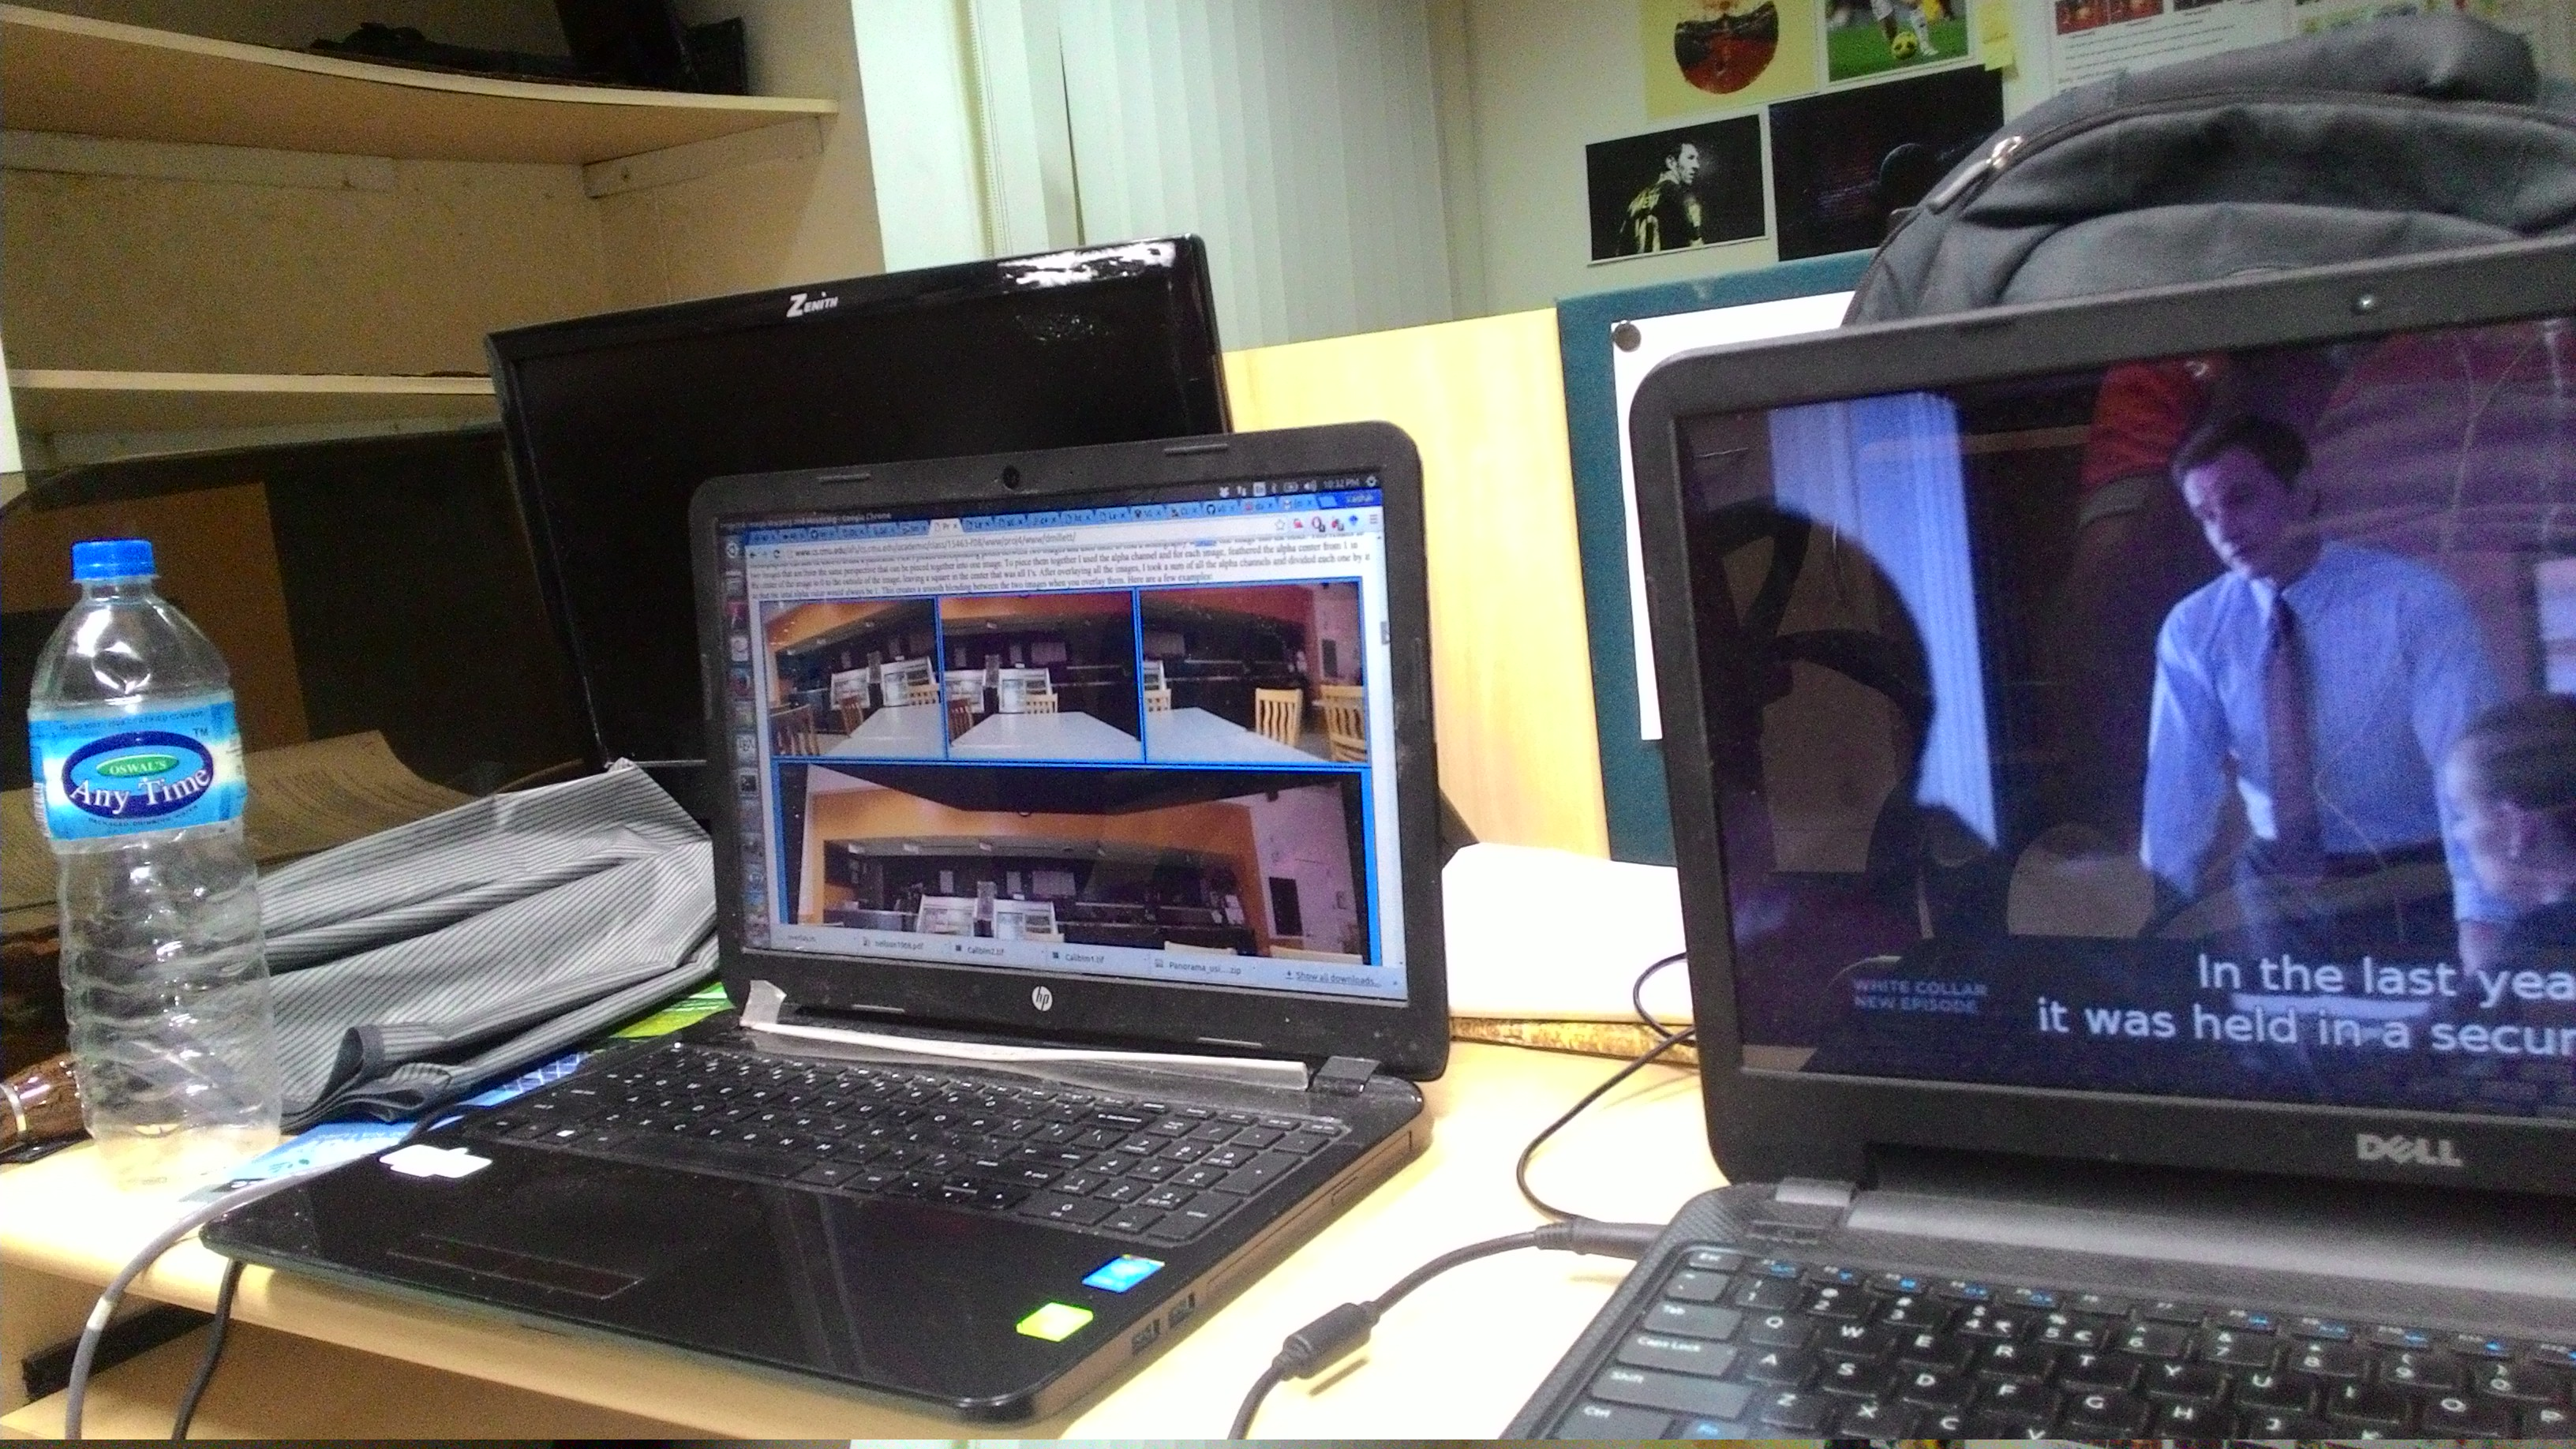
\includegraphics[scale = 0.067]{pt1.jpg}
\caption{Image 1}
\label{fig:Image 1}
\end{minipage}%
\begin{minipage}{.5\textwidth}
\centering
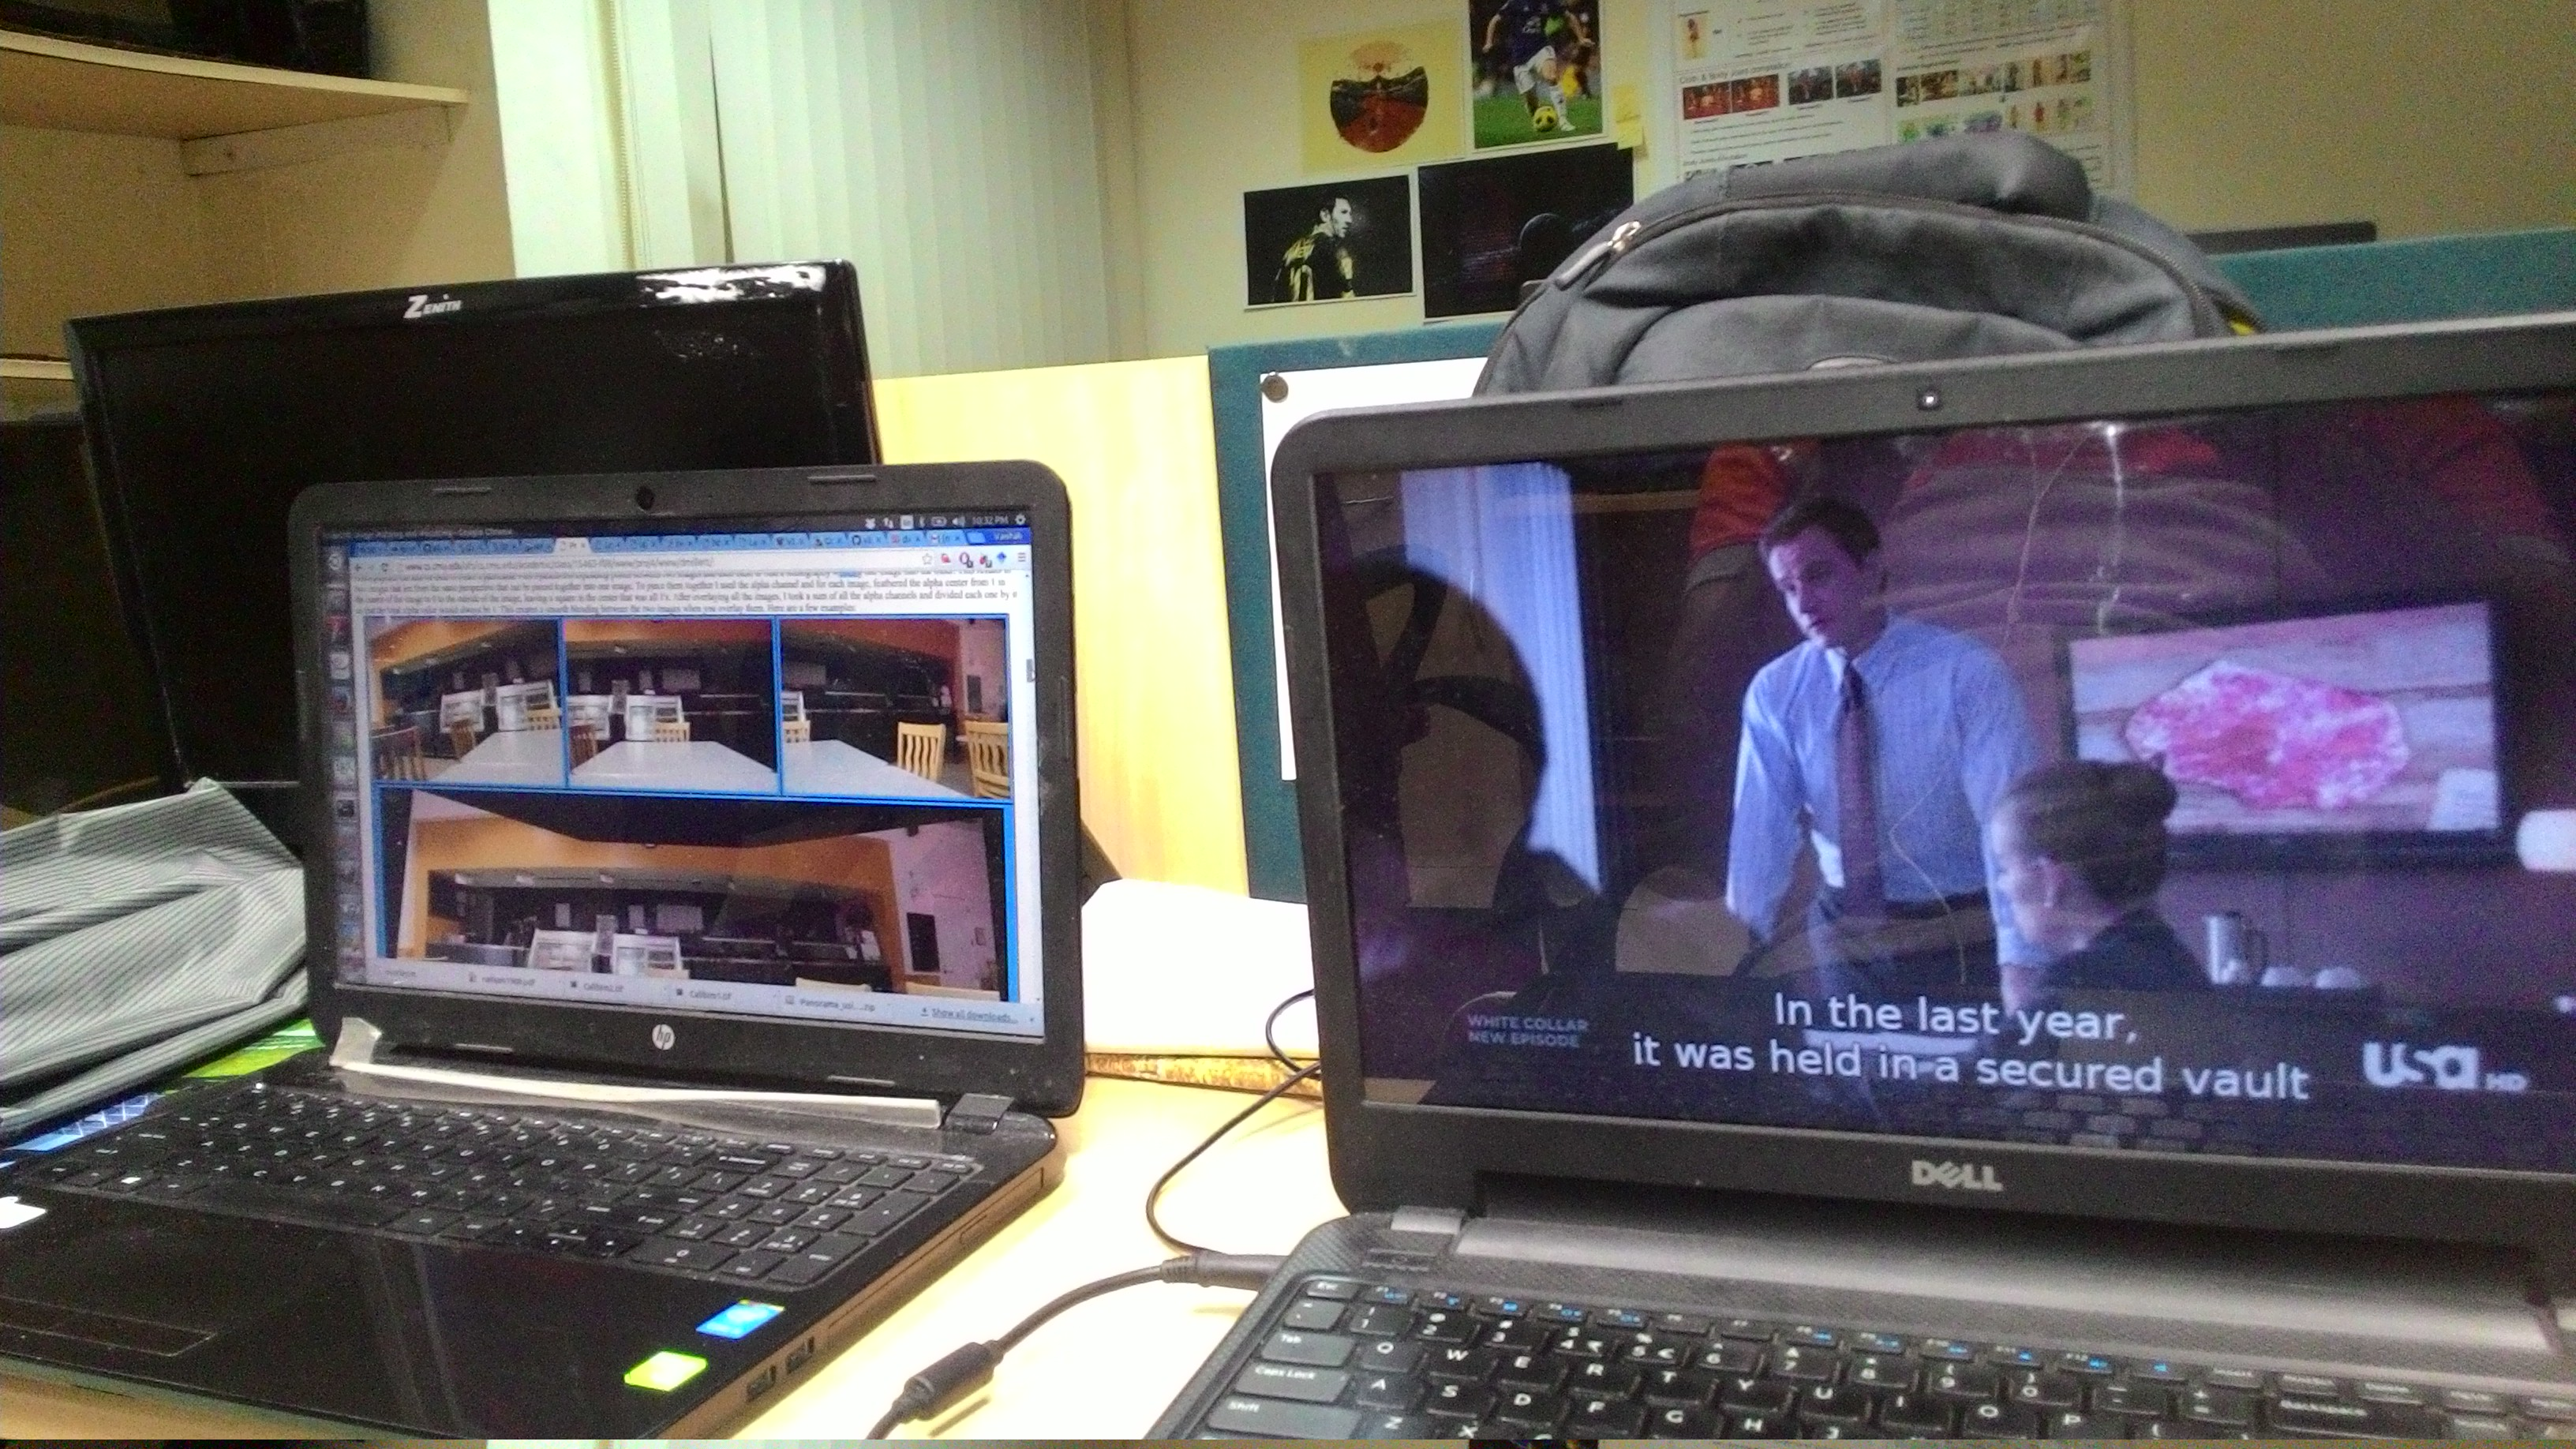
\includegraphics[scale = 0.067]{pt2.jpg}
\caption{Image 2}
\label{fig:Image 2}
\end{minipage}%
\end{figure}

\subsection{Output}
There were no re-projection error for the chosen image coordinates. It has been observed that DLT gives very high accuracy in estimating the camera parameters and thus very low re-projection error. The output image is shown in figure \ref{dltmanual}

The image coordinates of the corner points were as follows:
\begin{lstlisting}[language=matlab]
 imP2 = [658, 120, 1;
        784, 624, 1;
        402, 116, 1;
        1592, 164, 1;
        ];
  imP1 = [670, 120, 1;
        794, 622, 1;
        420, 118, 1;
        1592, 180, 1];
\end{lstlisting}

The parameters of the camera matrix are as follows:
\subsubsection{Camera Projection Matrix, P} 
\begin{tabular}{|c|c|c|}
\hline

  0.9756  &  -0.6560 &  37.9458 \\ 
  0.0164  &   0.4147 &  51.0405\\ 
  0.0000 &  -0.0008 &  1.0000
\\ 
\hline
\end{tabular}


\subsubsection{Intrinsic Parameters, K}
\begin{tabular}{|c|c|c|}
\hline

  -0.9923  &  0.5942 &  37.9464 \\ 
  0.0000  &   -0.4577 &  51.0401\\ 
  0.0000 &  0.0008 &  1.0000
\\ 
\hline
\end{tabular}



\subsubsection{Rotation Matrix, R}

\begin{tabular}{|c|c|c|}
\hline

  -0.9995 &  0.0304 &  -0.0008 \\ 
  -0.0304  &   -0.9995  &  51.0401\\ 
  0.0000 &  -0.0008 &  1.0000
\\ 
\hline
\end{tabular}

\subsubsection{Camera Center, C}
\begin{tabular}{|c|c|c|}
\hline

  -0.0000 & 0 & 1.0000 \\ 
\hline
\end{tabular}

\subsubsection{Observations}
There is some backprojection error in the estimated points from the homoraphy matrix as seen in figure \ref{dltmanual}

\subsubsection{Output Image}
\begin{figure}[htp]
\centering
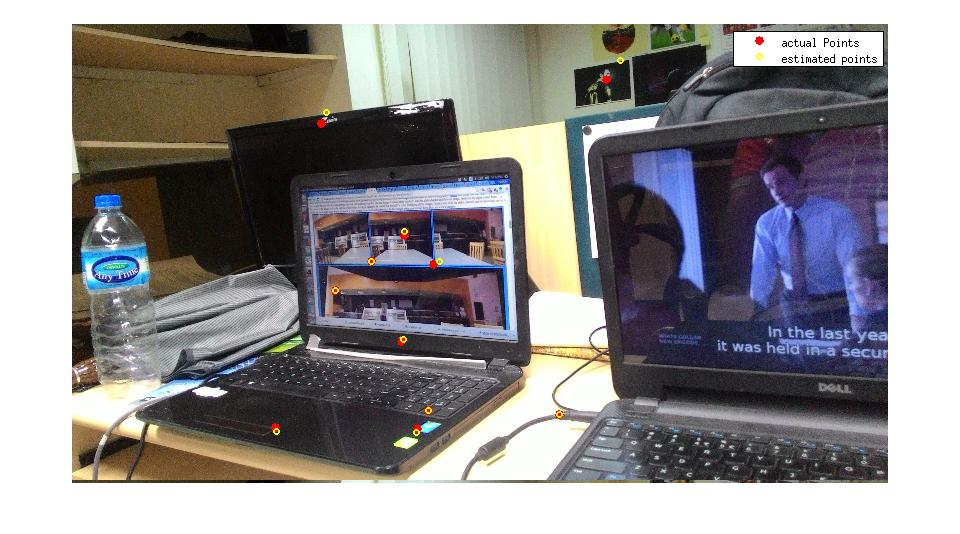
\includegraphics[width=1.3\textwidth]{dltPt2manual.jpg}\hfill
\caption{Estimated Points from Homography Matrix}
\label{dltmanual}
\end{figure}
\clearpage




\section{DLT with SIFT features}

\subsection{Code} 
\subsubsection{DLT code}
\begin{lstlisting}[language=matlab]

function p = dlt(imP2,imP1)

A = zeros(9,9);
    k = 1;
    for i = 1:4
        imPt = imP2(i, 1);
        A(k, 1:3) = -imP1(i,:);
        A(k,4:6) = zeros(1,3);
        A(k,7:9) = [imPt*imP1(i,1), imPt*imP1(i,2), imPt*imP1(i,3)];
        k = k + 1;

        imPt = imP2(i, 2);
        A(k,1:3) = zeros(1,3);
        A(k, 4:6) = -imP1(i,:);
        A(k,7:9) = [imPt*imP1(i,1), imPt*imP1(i,2), imPt*imP1(i,3)];
        k = k + 1;
    end

    [U, S, V] = svd(A);
    singV = diag(S);
    [~, indx] = sort(singV);
    p = V(:, indx(1));
    p = reshape(p, [3,3])';
    estimatedImg = p*imP1';
    imgEst = (estimatedImg ./ repmat(estimatedImg(3,:),3,1))';
    H = p(:,1:3);
    invH = inv(H);
    [invR, invK] = qr(invH);
    R = invR';
    K = inv(invK);
    C = invH*p(:,3);
end
\end{lstlisting}
\subsubsection{SIFT Code}
\begin{lstlisting}
function [im1Pts, im2Pts, Ia, Ib] = sift(Ia, Ib)
    
      if(size(Ia, 1) > 1000 || size(Ia, 2) > 1000)
          Ia = imresize(Ia, 0.5);
      end
     
      if(size(Ib, 1) > 1000 || size(Ib, 2) > 1000)
          Ib = imresize(Ib, 0.5);
      end
    [fa,da] = vl_sift(im2single(rgb2gray(Ia))) ;
    [fb,db] = vl_sift(im2single(rgb2gray(Ib))) ;

    [matches, scores] = vl_ubcmatch(da,db) ;

    [drop, perm] = sort(scores, 'ascend') ;
    matches = matches(:, perm) ;
    scores  = scores(perm) ;

    sz = min(100, length(scores));
    matches = matches(:,1:sz);
    scores = scores(1:sz);

    im1Pts = fa(1:2,matches(1,:));
    im2Pts = fb(1:2,matches(2,:));
    
    im1Pts = [im1Pts; ones(1, size(im1Pts,2))];
    im1Pts = im1Pts';
    im2Pts = [im2Pts; ones(1, size(im2Pts,2))];
    im2Pts = im2Pts';
     
    m = size(im1Pts,1);
    indices = randperm(m, 4);
   	imP1 = im1Pts(indices,:);
   	imP2 = im2Pts(indices, :);

    p = dlt(imP2,imP1);

    
   estI2 = p*im1Pts';
   estI2 = (estI2 ./ repmat(estI2(3,:),3,1))';
   figure;
   imshow(Ib);

   hold on;
   plot(im2Pts(:,1), im2Pts(:,2), 'r*', 'LineWidth',3);
   plot(estI2(:,1), estI2(:,2), 'bo', 'LineWidth',2); 
   legend('actual Points','estimated points') 
    \end{lstlisting}
\subsection{Input}
The input to RANSAC are a set of 2 images for estimating the homography. The images are taken by rotating the camera by an angle. The input images are shown in figures \ref{dltsiftInput1}, \ref{dltsiftInput2}.

\begin{figure}[h]
\centering
\begin{minipage}{0.6\textwidth}
\centering
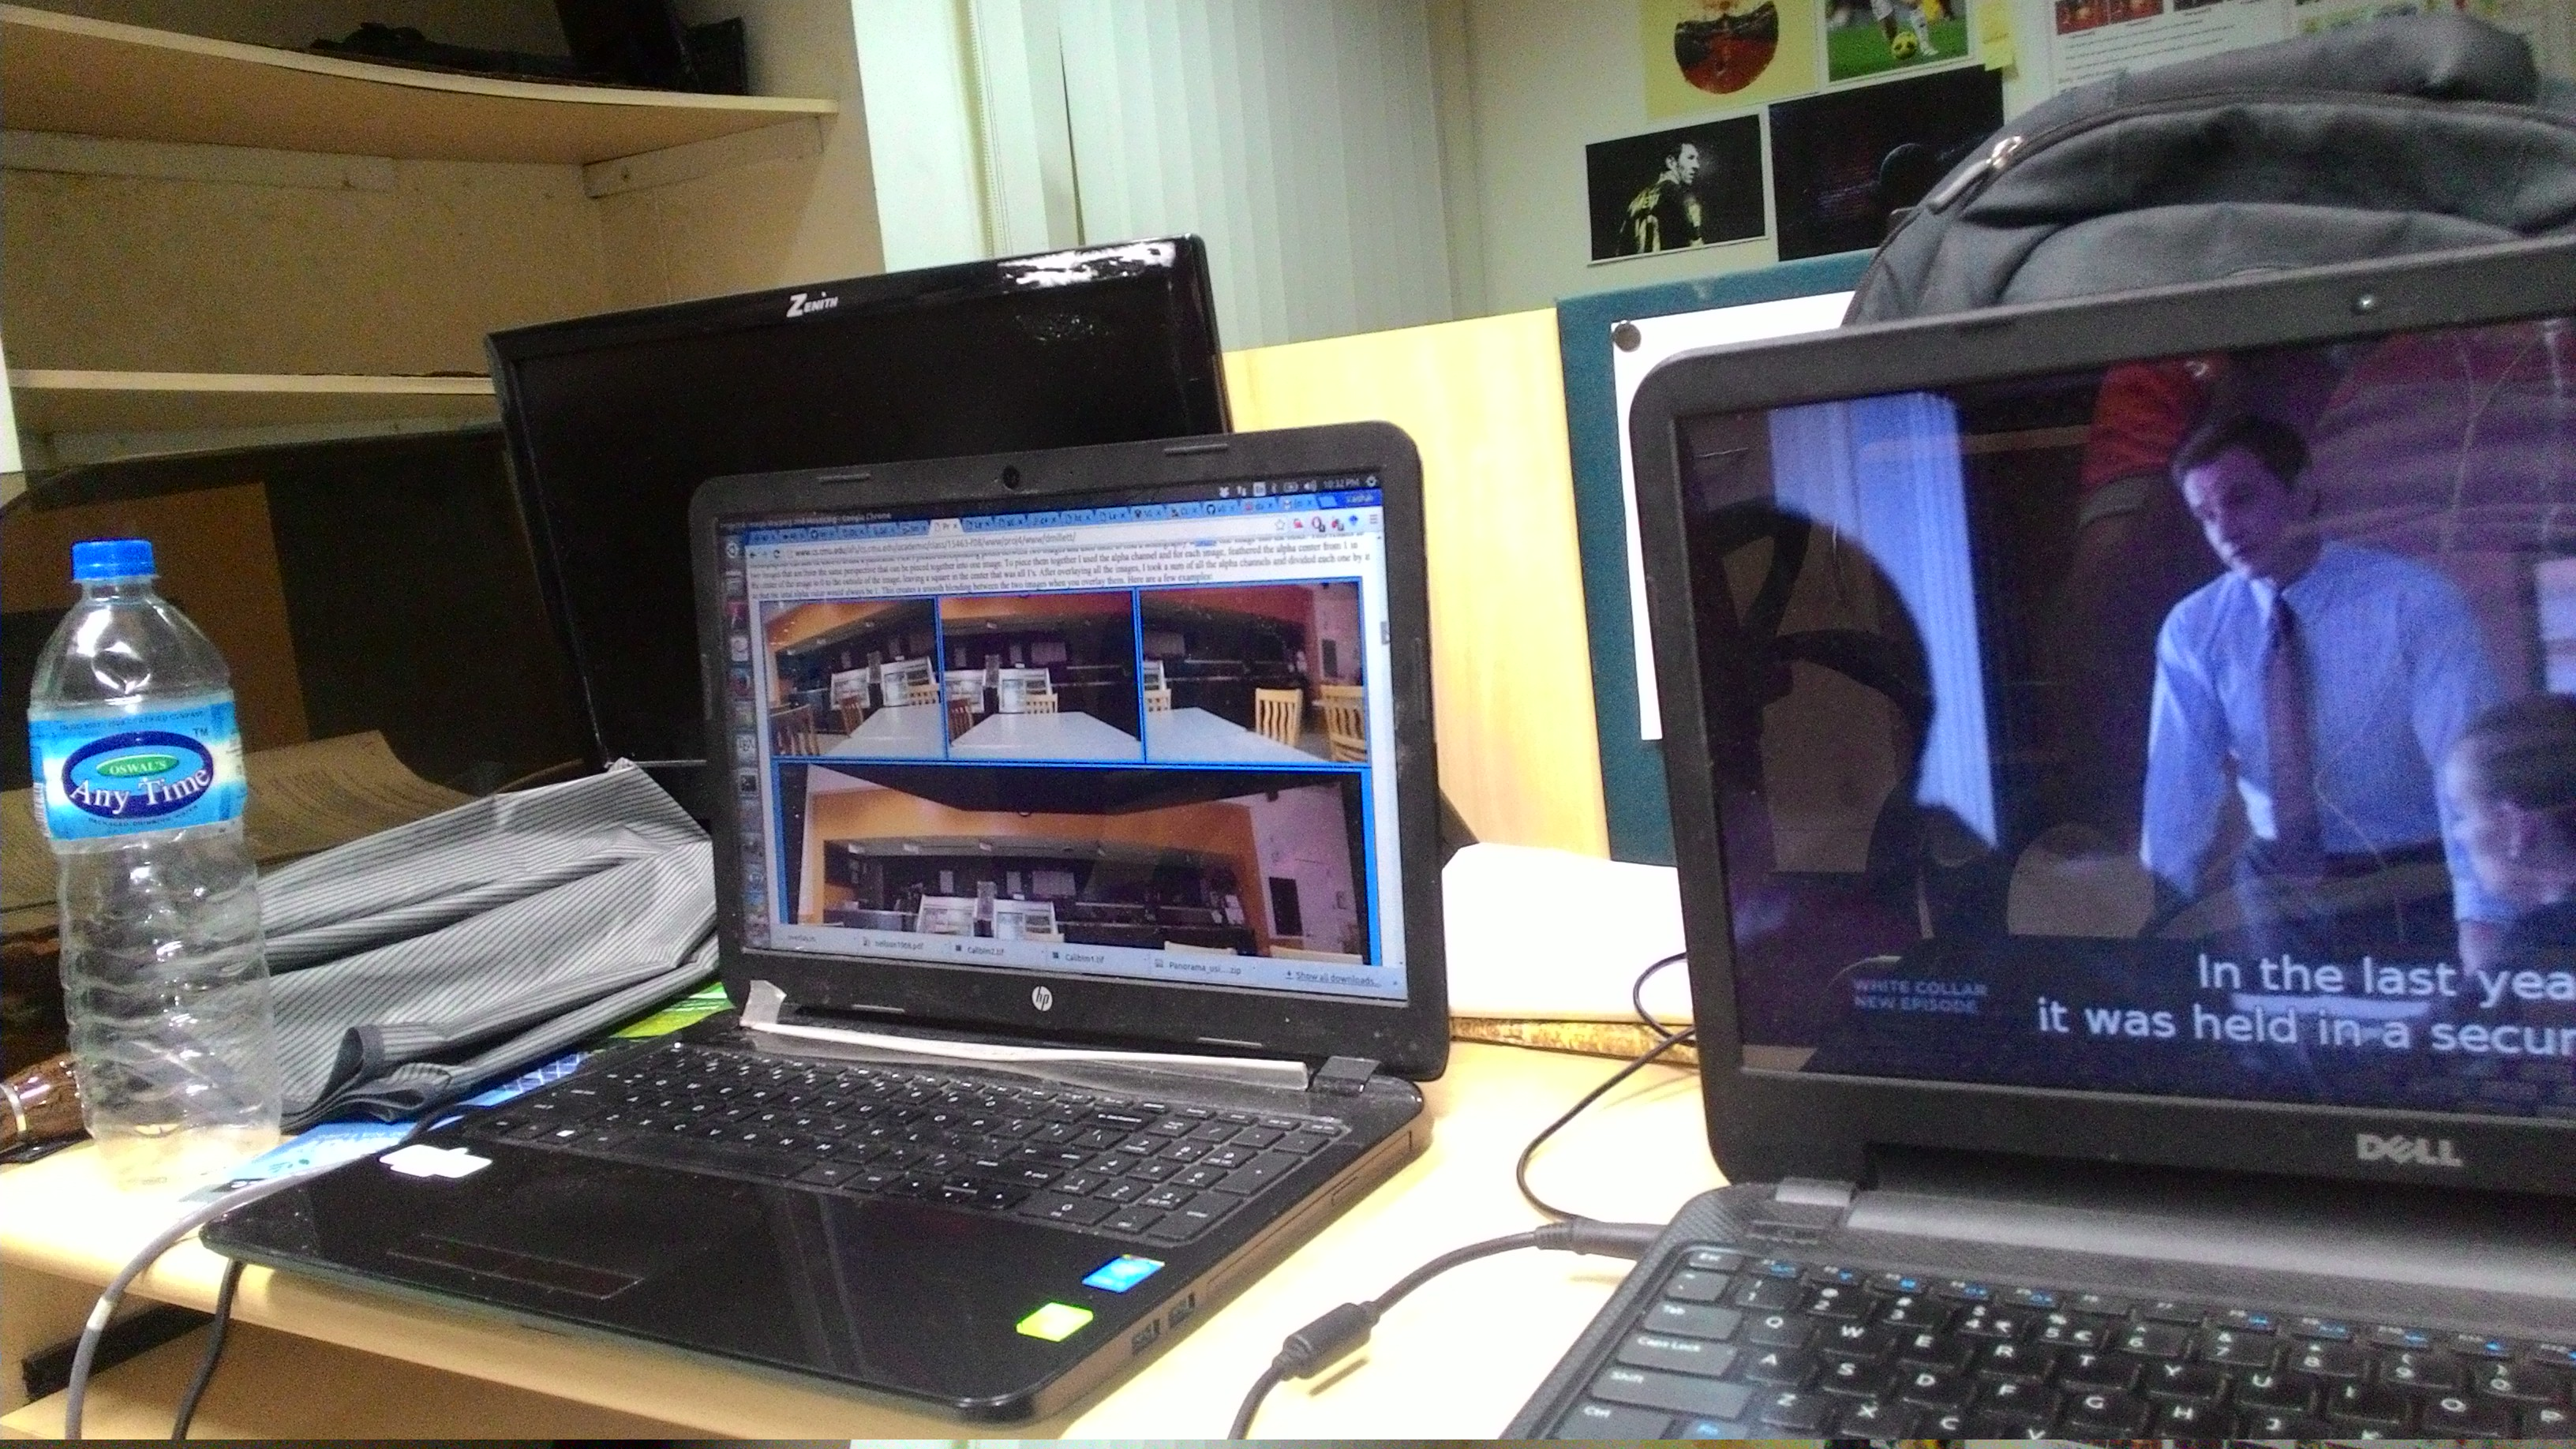
\includegraphics[scale = 0.067]{pt1.jpg}
\caption{Image 1}
\label{dltsiftInput1}
\end{minipage}%
\begin{minipage}{.5\textwidth}
\centering
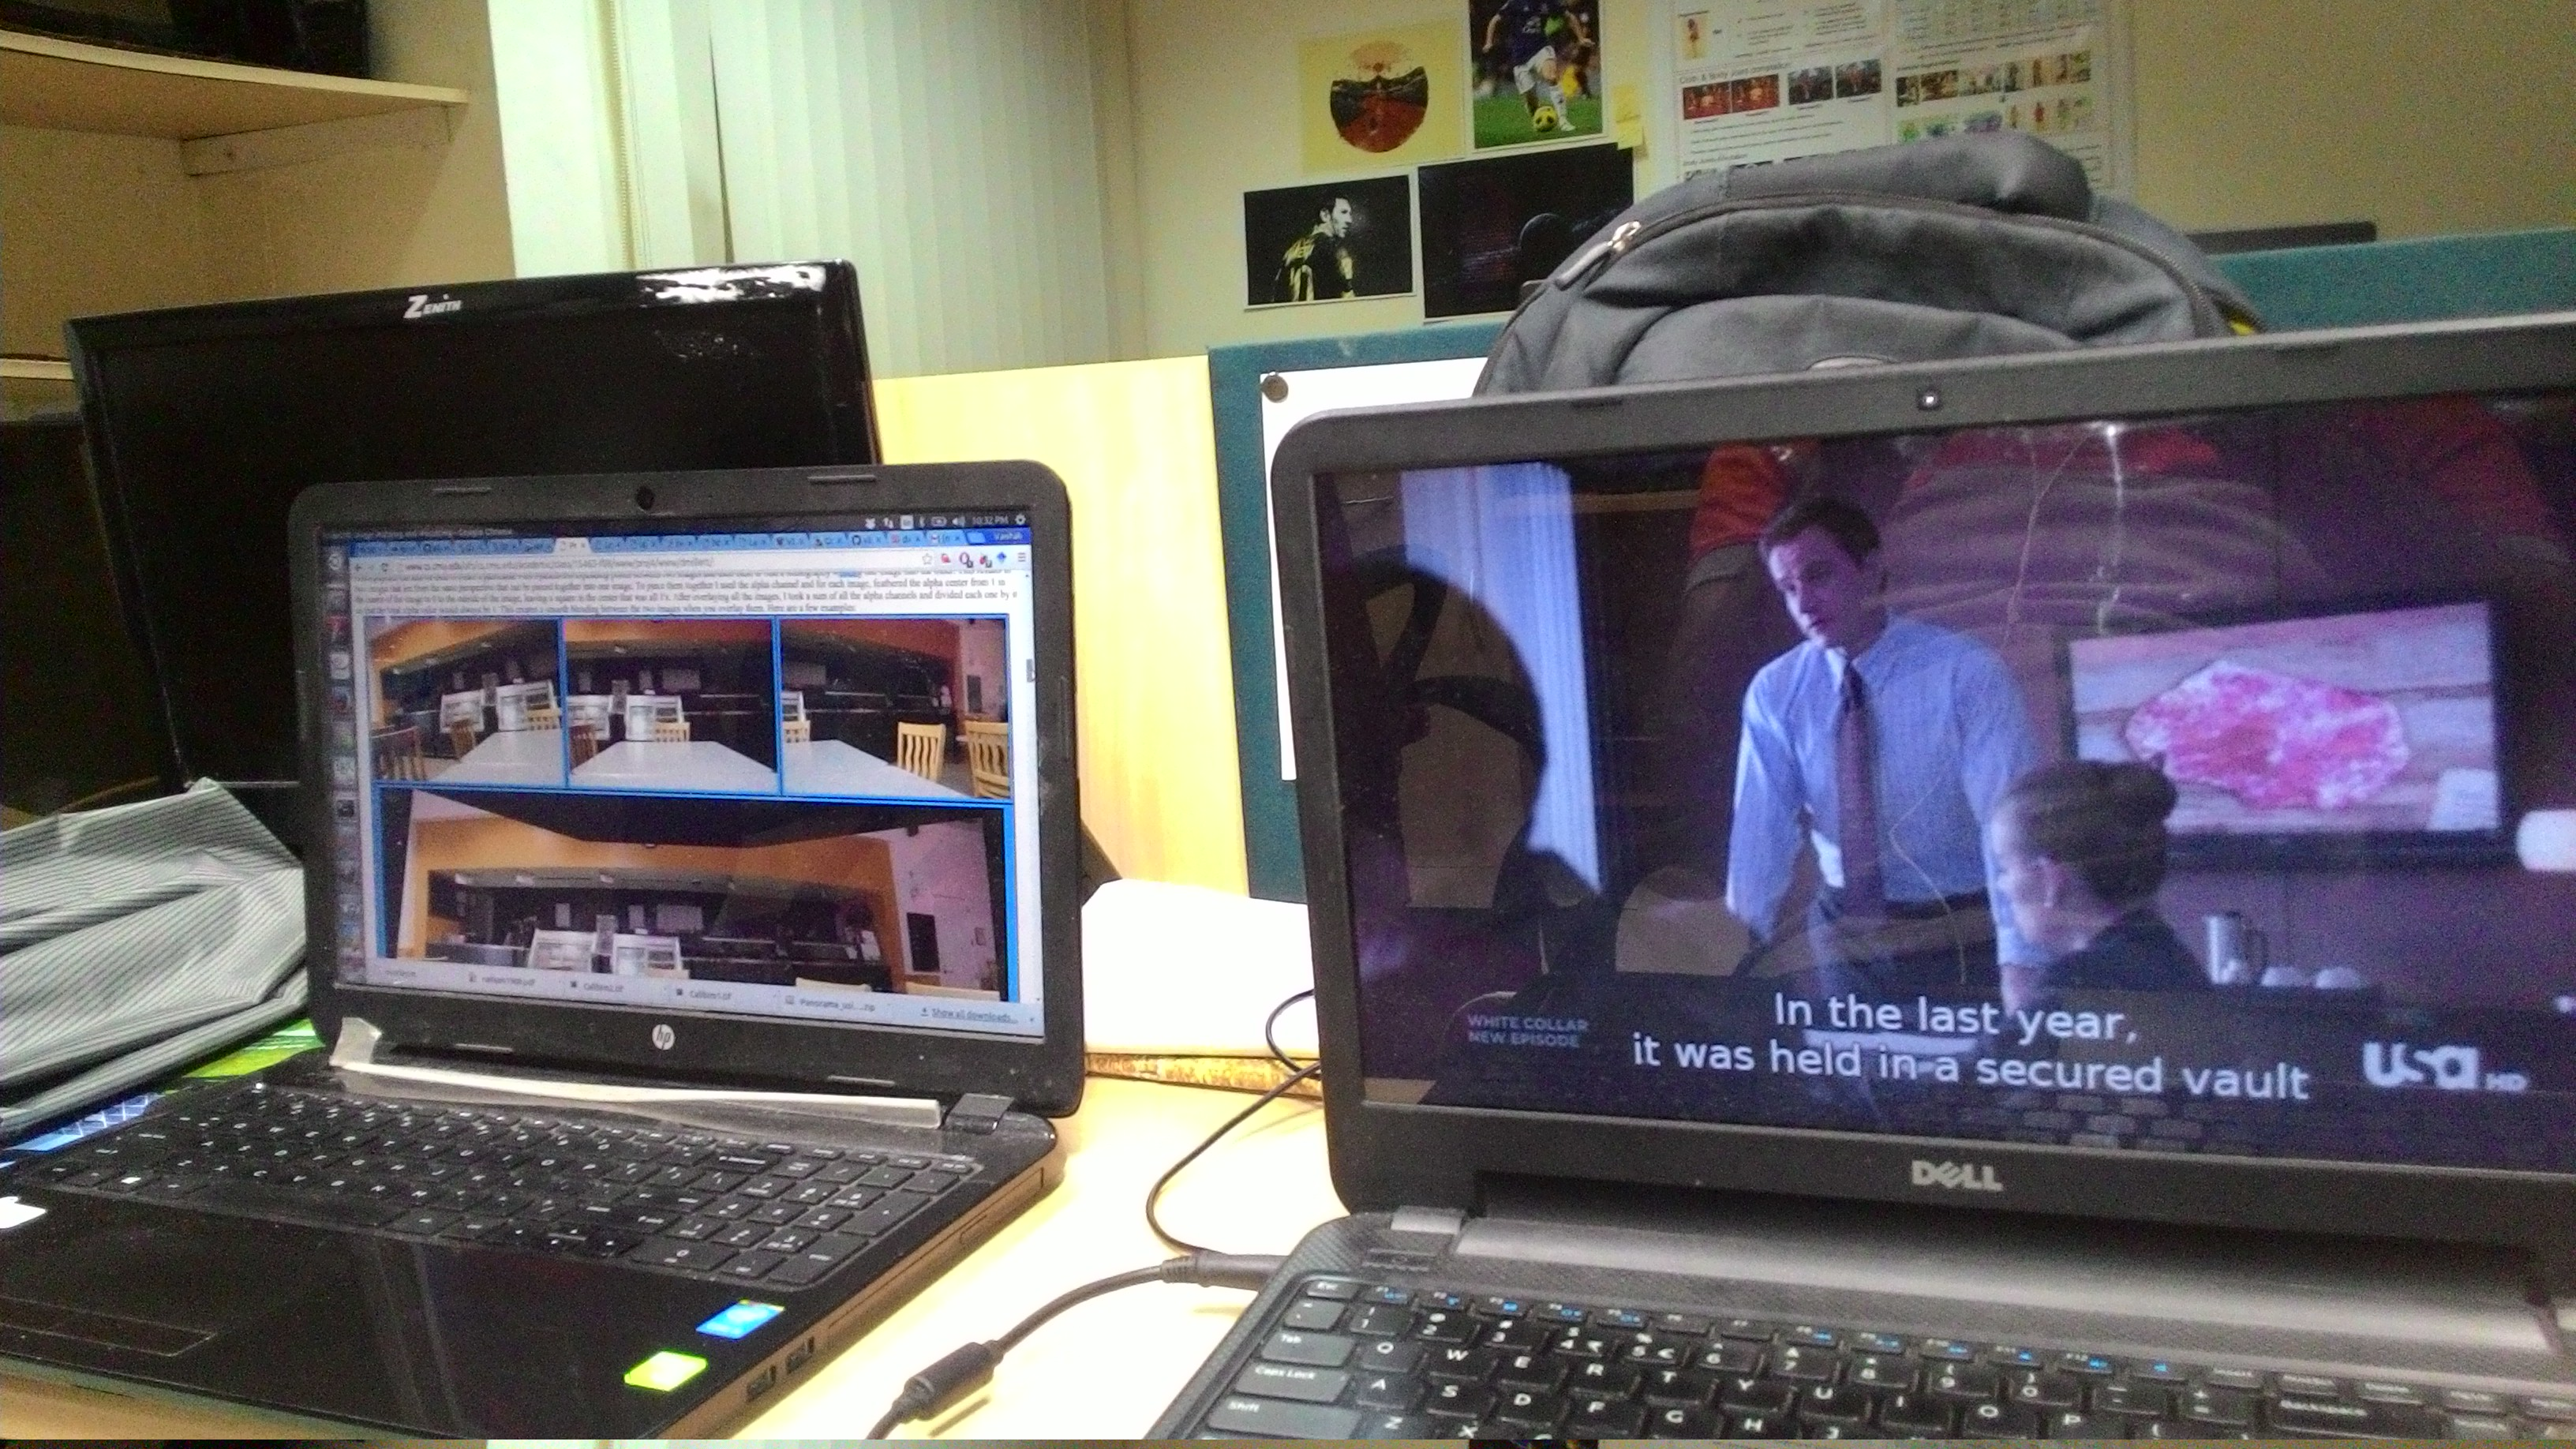
\includegraphics[scale = 0.067]{pt2.jpg}
\caption{Image 2}
\label{dltsiftInput2}
\end{minipage}%
\end{figure}
\clearpage

\subsection{Output}

The parameters of the homography matrix are as follows:

\subsubsection{Camera Projection Matrix, P} 
\begin{tabular}{|c|c|c|}
\hline

 0.9943   &  0.0050 &  8.8669 \\ 
  0.0145  &  0.9974 &  -3.6872\\ 
  0.0000 &  0.0000 &  1.0000
\\ 
\hline
\end{tabular}
        

\subsubsection{Intrinsic Parameters, K}
\begin{tabular}{|c|c|c|}
\hline

 -0.9941  &  -0.0193  &  8.8669 \\ 
  0  &  -0.9975 &  -3.6872\\ 
  0.0000 &  0.0000 &  1.0000
\\ 
\hline
\end{tabular}

\subsubsection{Rotation Matrix}
\begin{tabular}{|c|c|c|}
\hline

 -0.9999  &  0.0145 &  0.0000 \\ 
  -0.0145   &  -0.9999 &  0.0000\\ 
  0.0000 &  0.0000 &  1.0000
\\ 
\hline
\end{tabular}
         

\subsubsection{Center of Camera}
\begin{tabular}{|c|c|c|}
\hline

 0  &  0 &  1.0000 \\ 
  \hline
\end{tabular}


\subsubsection{Observations}
There is some backprojection error in the estimated points from the homoraphy matrix as seen in figure \ref{dltmanual}

\subsubsection{Output Image}
The matched points of SIFT are shown in figure \ref{sift} and the estimated points from the homography matrix is shown in the figure  \ref{dltsift}




\begin{figure}[htp]
\centering
\begin{minipage}{1.0\textwidth}
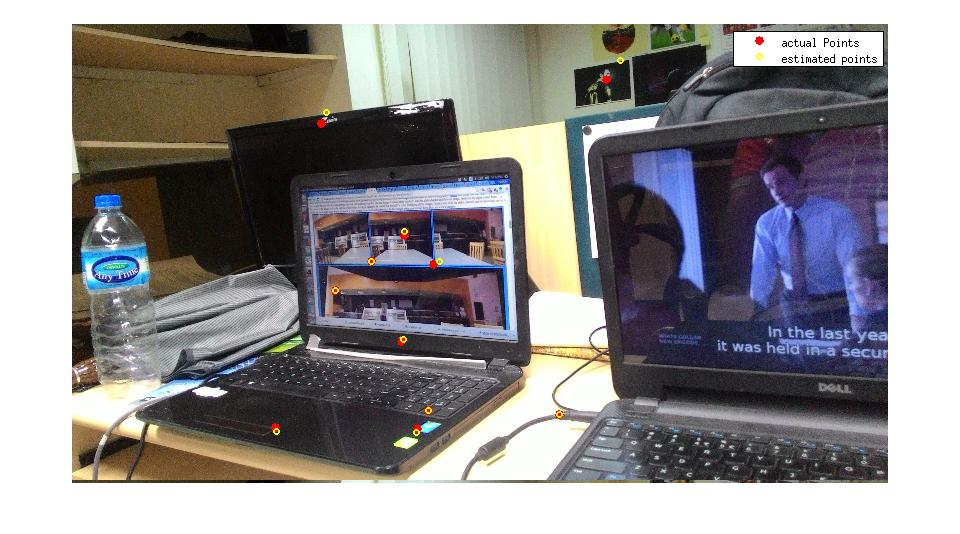
\includegraphics[width=1.3\textwidth]{dltPt2manual.jpg}\hfill
\label{dltmanual}
\caption{Estimated Points from Homography Matrix}
\end{minipage}

\centering
\begin{minipage}{1.0\textwidth}
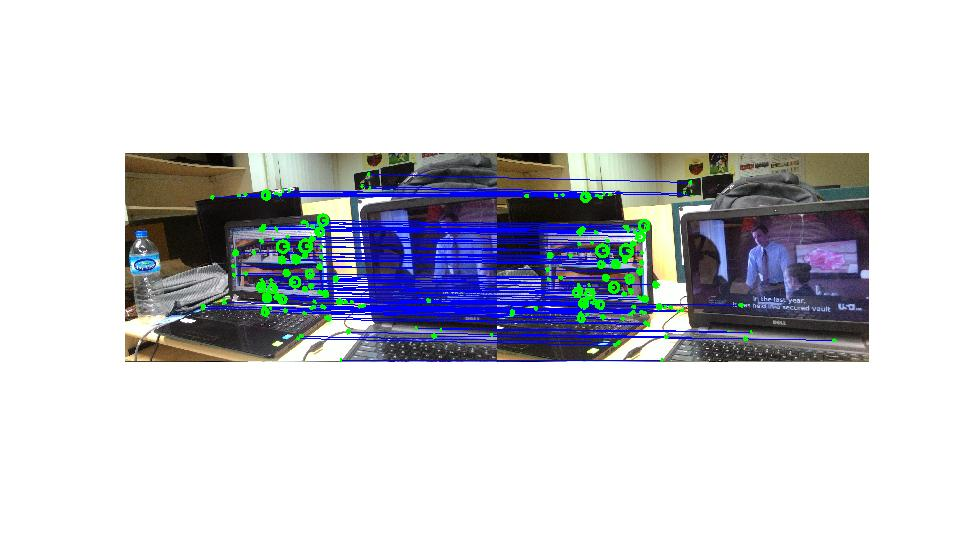
\includegraphics[width=1.0\textwidth]{siftPt.jpg}\hfill
\caption{Matched points from SIFT}
\label{dltsift}

\end{minipage}
\end{figure}



\clearpage



\section{RANSAC with manual features}
Random sample consensus (RANSAC) is an iterative method to estimate parameters of a mathematical model from a set of observed data which contains outliers. RANSAC is used for camera calibration to estimate the camera matrix with the least re-projection error.
The best estimation of the camera matrix is chosen to be the one with minimum number of outliers.



\subsection{Code} 
\subsubsection{RANSAC code}
\begin{lstlisting}[language=matlab]

   img2Pts = [658, 120, 1;
        784, 624, 1;
        402, 116, 1;
        1592, 164, 1;
         
        318, 746, 1;
         576, 136, 1;
         712, 254, 1;
         610, 190, 1;
         484, 258, 1
        ];
    img1Pts = [670, 120, 1;
        794, 622, 1;
        420, 118, 1;
        1592, 180, 1;

        336, 754, 1;
        592, 140, 1;
        726, 258, 1;
        622, 188, 1;
        496, 254, 1
      ];

err = 0;
mnErr = 5000000;
p = zeros(3,3);

m = size(img1Pts,1);
n = randperm(m);

im1 = img1Pts(n,:);
im2 = img2Pts(n,:);
choseni = 1;
for iter = 1:10
    
   indices = randperm(m, 4);
   imP1 = im1(indices,:)
   imP2 = im2(indices, :)
    P = dlt(imP2, imP1);
   estimatedI2 = P*im1';
   estimatedI2 = round(estimatedI2 ./ repmat(estimatedI2(3,:),3,1))';
   err = sum(sqrt(sum((im2 - estimatedI2).^2,2)))/m;
   if mnErr >= err
       p = P;
       mnErr = err;
       choseni = iter;
   end
   
end

mnErr
'finalP'
p
estimatedImg = p*img1Pts';
imgEstimated = round(estimatedImg ./ repmat(estimatedImg(3,:),3,1))';
H = p(:,1:3);
invH = inv(H);
[invR, invK] = qr(invH);
 R = invR'
 K = inv(invK)
 C = invH*p(:,3)


figure;
imshow(I1);
hold on;
plot(img2Pts(:,1), img2Pts(:,2), 'r*', 'LineWidth',3);
plot(imgEstimated(:,1), imgEstimated(:,2), 'bo', 'LineWidth',2);  
legend('actual Points','estimated points')  

\end{lstlisting}

\subsection{Input}
The experiment was performed with 2 sets of images. One set has the camera slightly rotated. The other set has significant rotation and translation of the camera.
The input to RANSAC are a set of 2 images for estimating the homography. The images are taken by rotating the camera by a slight angle.

\begin{figure}[h]
\centering
\begin{minipage}{0.6\textwidth}
\centering
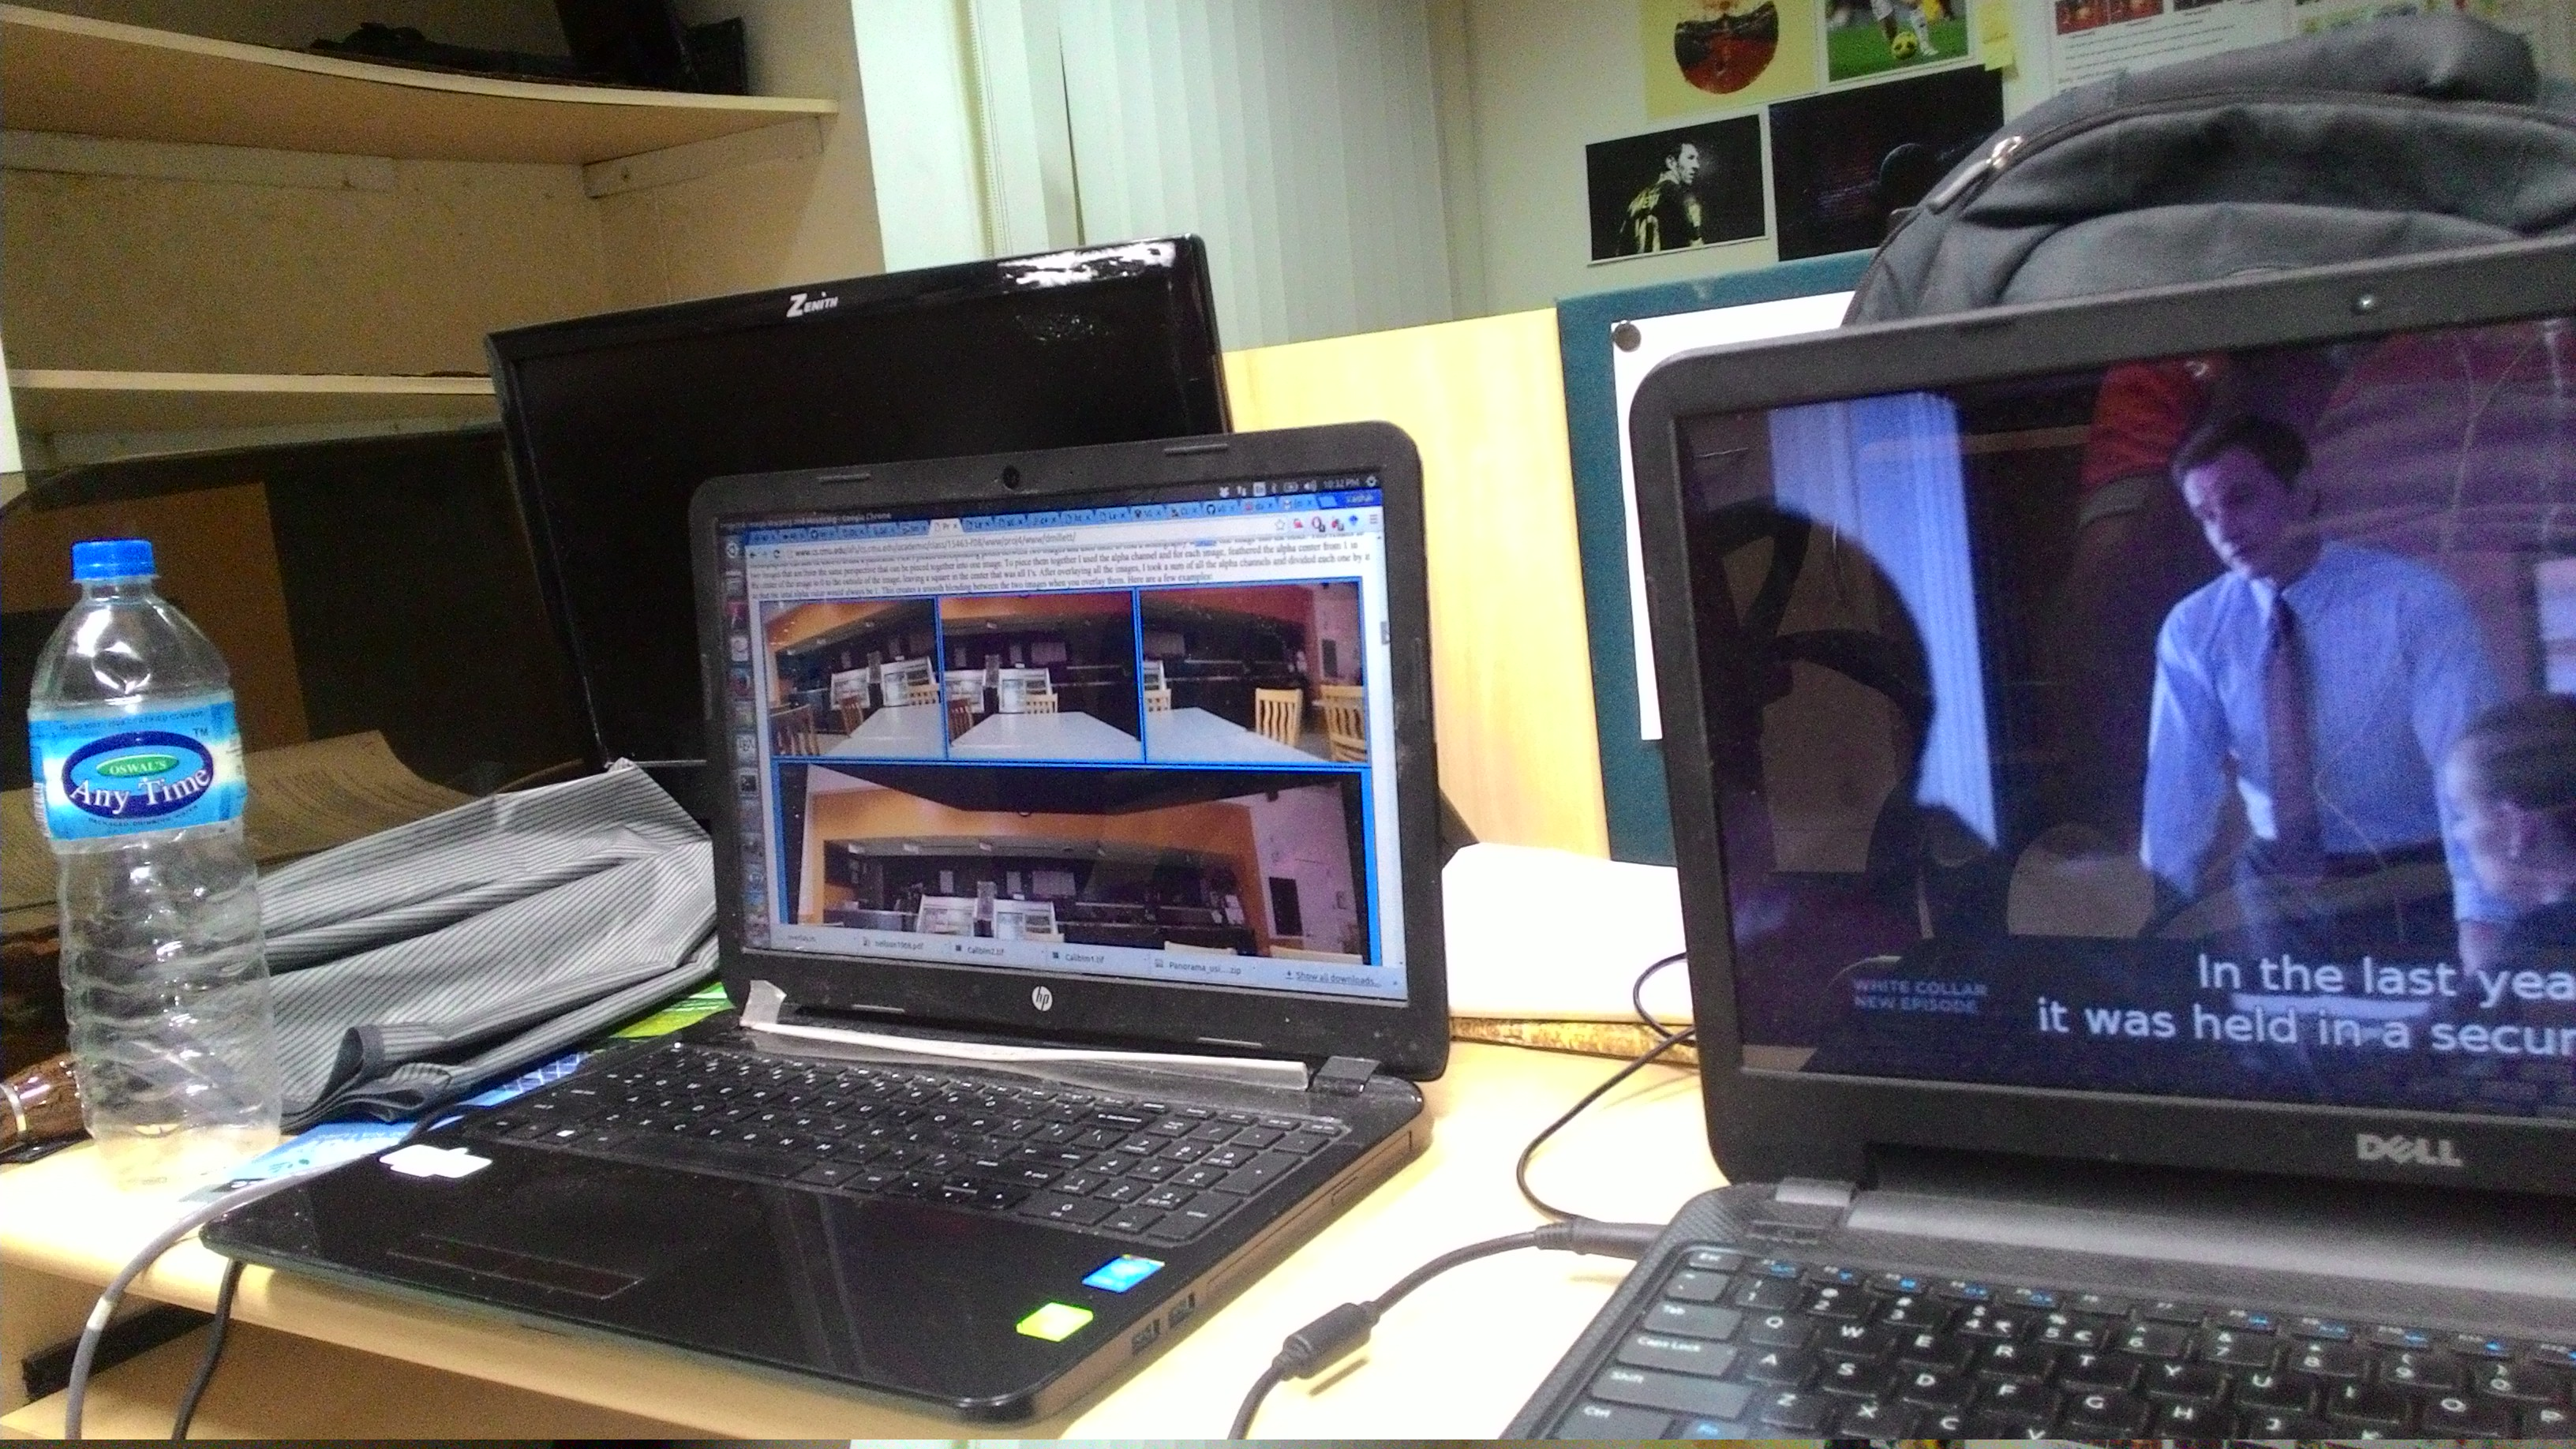
\includegraphics[scale = 0.067]{pt1.jpg}
\caption{Image 1}
\label{fig:Image 1}
\end{minipage}%

\begin{minipage}{.5\textwidth}
\centering
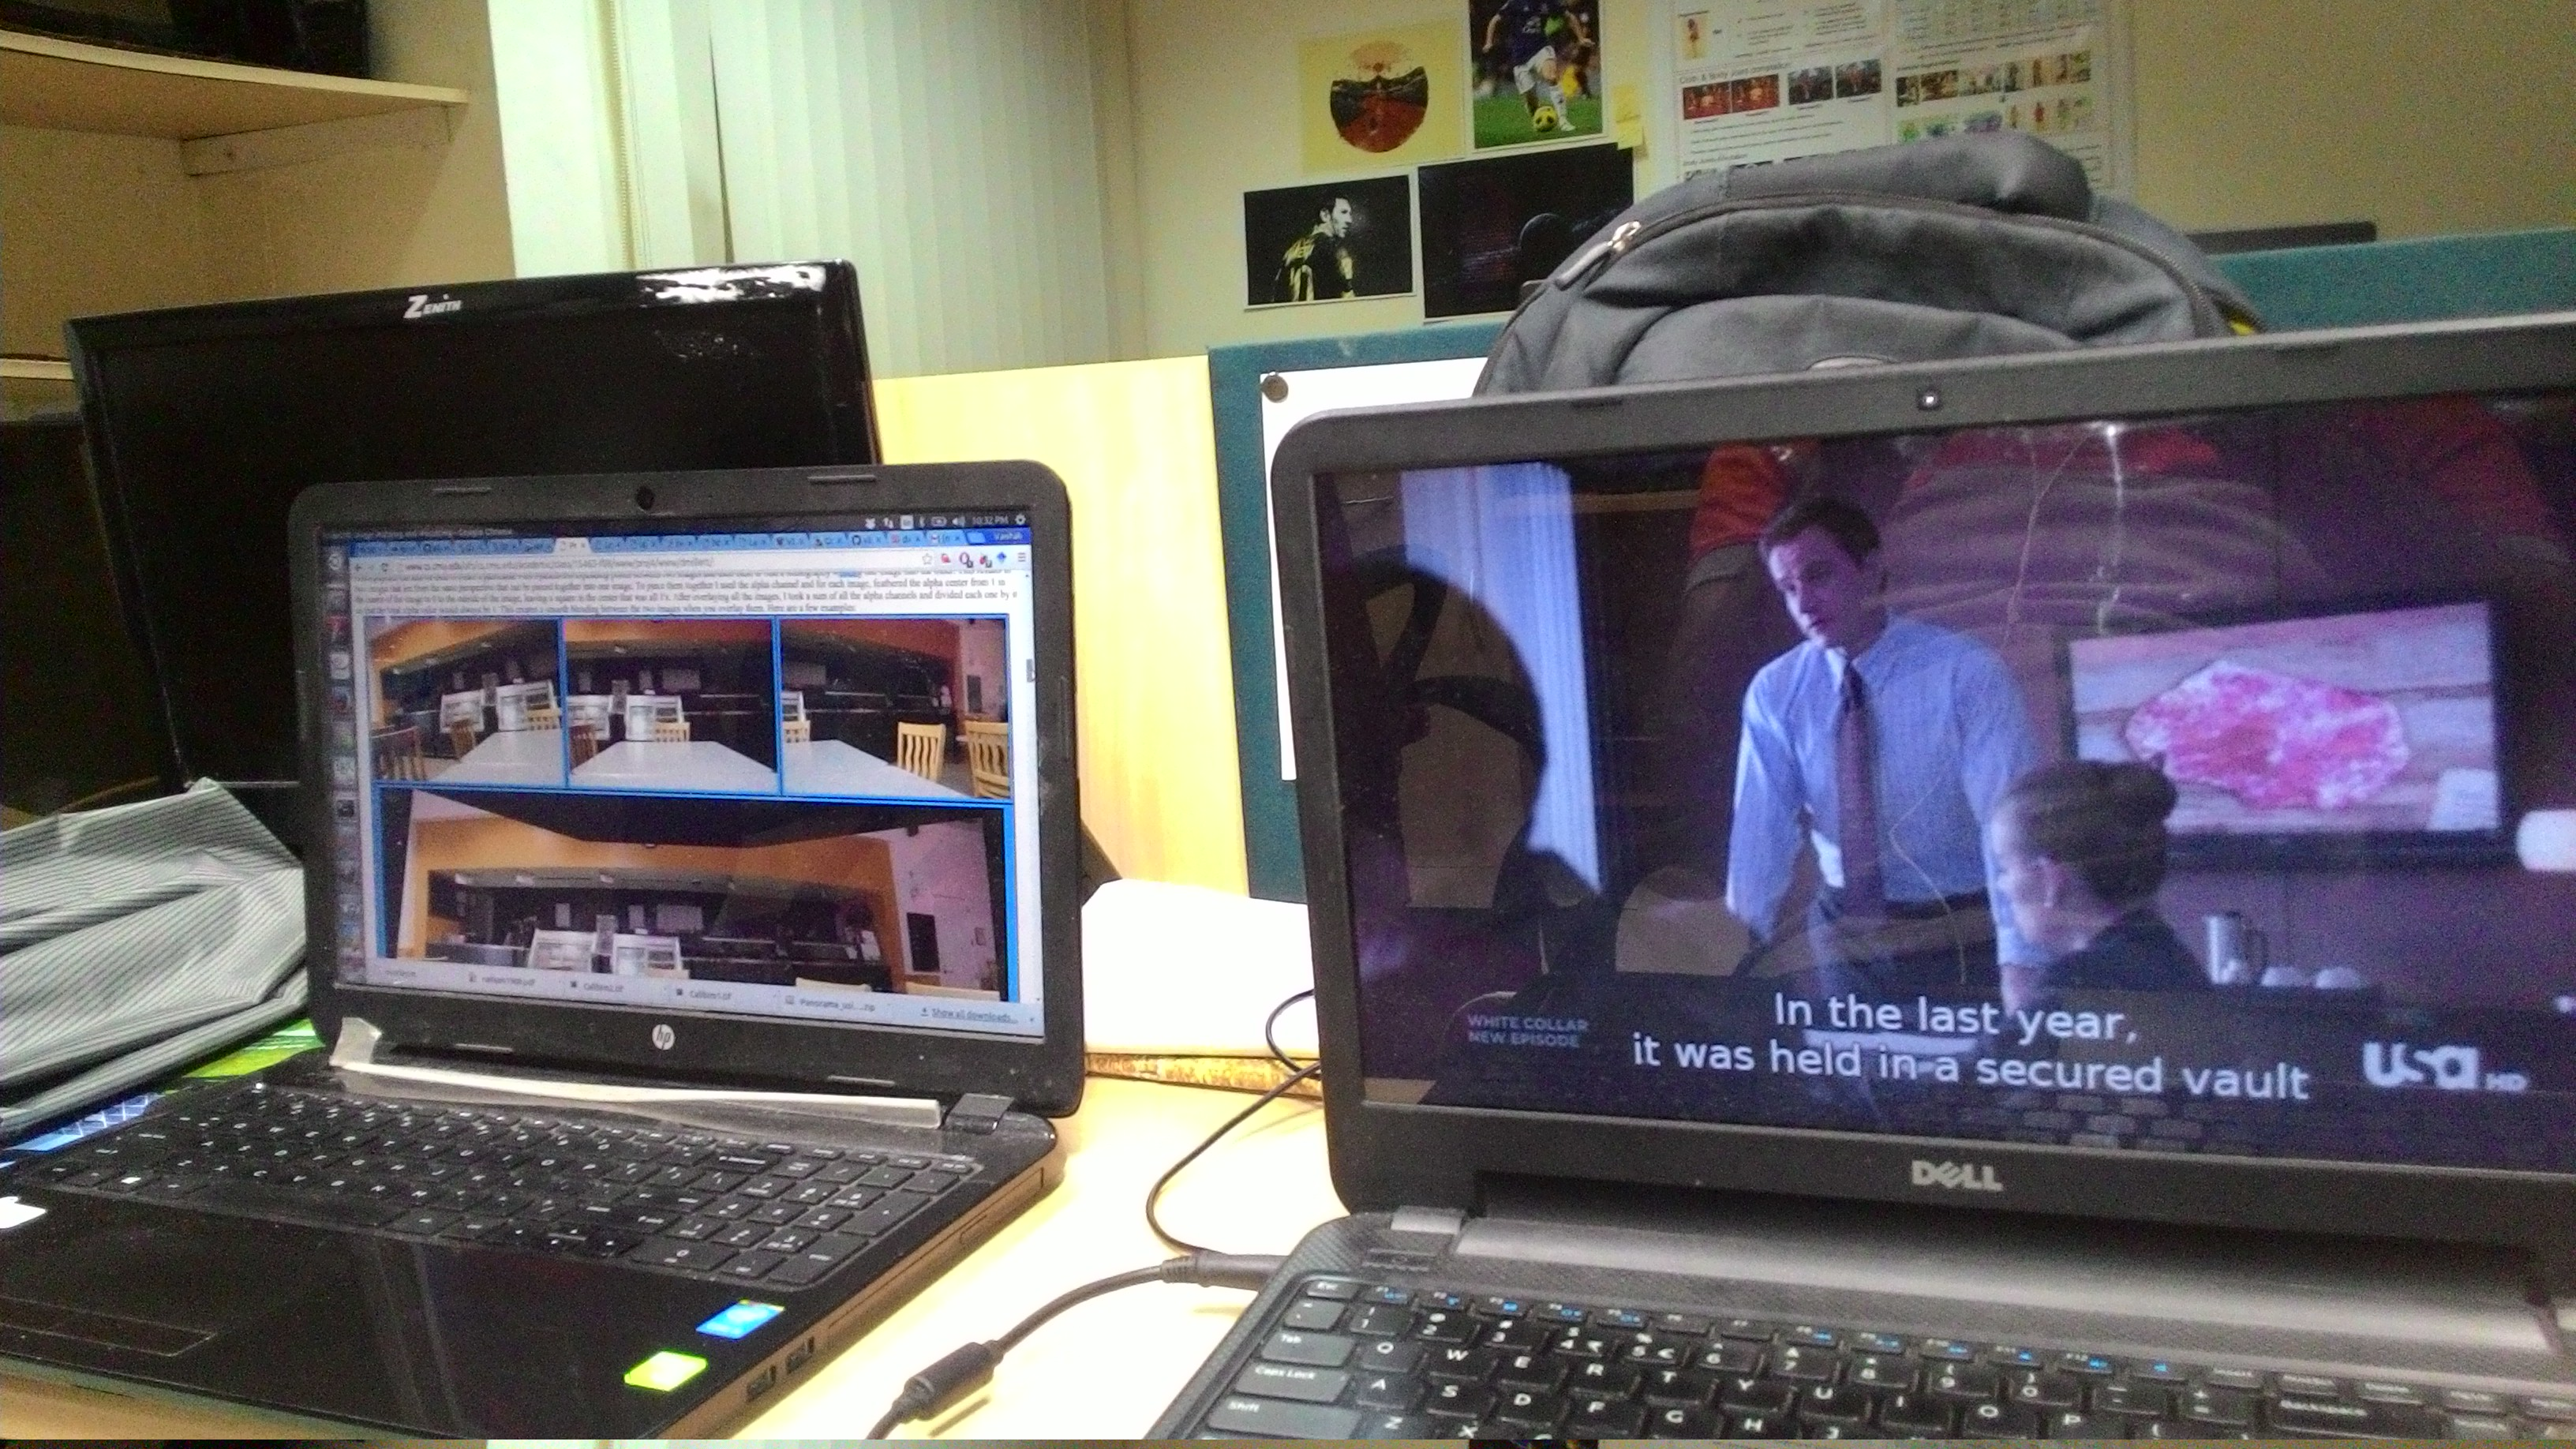
\includegraphics[scale = 0.067]{pt2.jpg}
\caption{Image 2}
\label{fig:Image 2}
\end{minipage}%
\end{figure}
\clearpage

\subsection{Output}

The parameters of the camera matrix are as follows:
\subsubsection{Camera Projection Matrix, P} 
\begin{tabular}{|c|c|c|}
\hline

0.7673 &  0.0219 &  536.5077 \\
 -0.0914 &  0.8782 &  89.4558 \\
 -0.0001 &  0 &  1 \\
\hline
\end{tabular}
                  
               
\subsubsection{Intrinsic Parameters, K}
\begin{tabular}{|c|c|c|}
\hline

 -0.8078 &  0.0492 &  536.5077 \\
 0 &  -0.8833 &  89.4558 \\
 0 &  0 &  1 \\
\hline
\end{tabular}
     
        
\subsubsection{Rotation Matrix}
\begin{tabular}{|c|c|c|}
\hline
-0.9954 &  -0.0957 &  -0.0001 \\
 0.0957 &  -0.9954 &  0 \\
 -0.0001 &  0 &  1 \\
\hline
\end{tabular}
             

\subsubsection{Center of Camera}
\begin{tabular}{|c|c|c|}
\hline

 0  &  0 &  1.0000 \\ 
  \hline
\end{tabular}



\subsubsection{Output Image}

\begin{figure}[htp]
\centering
\begin{minipage}{1.0\textwidth}
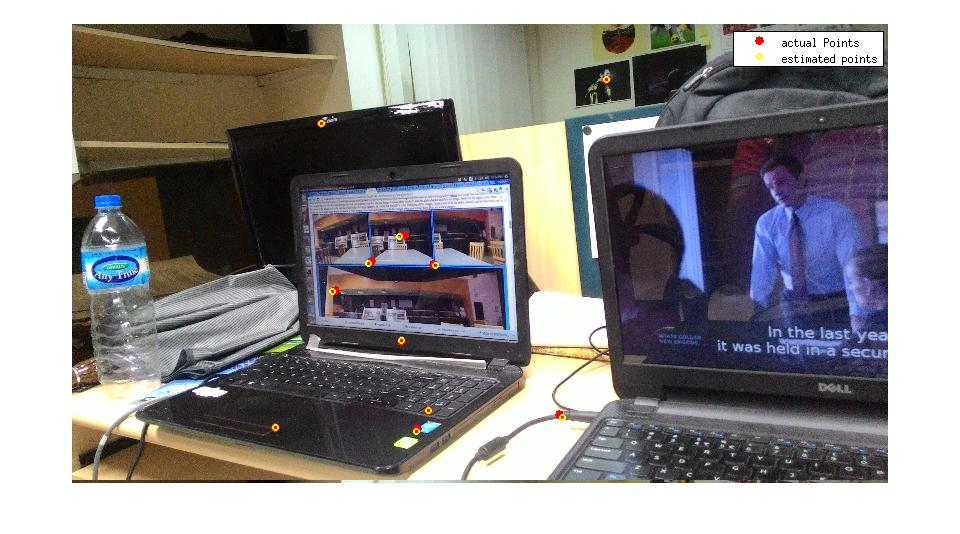
\includegraphics[width=1.3\textwidth]{ransacPtmanual.jpg}\hfill
\end{minipage}
\end{figure}
\clearpage
 
\section{RANSAC with SIFT features}
Random sample consensus (RANSAC) is an iterative method to estimate parameters of a mathematical model from a set of observed data which contains outliers. RANSAC is used for camera calibration to estimate the camera matrix with the least re-projection error.
The best estimation of the camera matrix is chosen to be the one with minimum number of outliers.



\subsection{Code} 
There are 3 source code scripts for RANSAC with SIFT
\begin{itemize}
\item mainCode - calls SIFT and RANSAC
\item SIFT - Performs feature dectection and matching
\item RANSAC - estimates the homography from matched features
\end{itemize}


\subsubsection{mainCode}
\begin{lstlisting}[language=matlab]
Ia = imread('pt1.jpg');
Ib = imread('pt2.jpg');
[im1Pts, im2Pts, Ia, Ib] = sift(Ia, Ib);

im1Pts = [im1Pts; ones(1, size(im1Pts,2))];
im1Pts = im1Pts';
im2Pts = [im2Pts; ones(1, size(im2Pts,2))];
im2Pts = im2Pts';

 

[p, K, R, C, imgEstimated] = ransac(im2Pts, im1Pts, Ib, Ia);
 estimatedImg = p*im1Pts';
imgEstimated = round(estimatedImg ./ repmat(estimatedImg(3,:),3,1))';

figure;
imshow(Ia);
hold on;
plot(im2Pts(:,1), im2Pts(:,2), 'r*', 'LineWidth',5);
plot(imgEstimated(:,1), imgEstimated(:,2), 'yo', 'LineWidth',2);  
legend('actual Points','estimated points')  
\end{lstlisting}

\vspace{2em}
\subsubsection{RANSAC code}
\begin{lstlisting}[language=matlab]
err = 0;
mnErr = 5000000;
p = zeros(3,3);

m = size(img1Pts,1);
n = randperm(m);

im1 = img1Pts(n,:);
im2 = img2Pts(n,:);
choseni = 1;

ptsChosenIndx = [];
outlierIn = [];
for iter = 1:10
    
   indices = randperm(m, 4);
   while((ismember(indices, outlierIn) == repmat([1], 1, 4)))
       indices = randperm(m,4);
       oulierIn
   end
   imP1 = im1(indices,:);
   imP2 = im2(indices, :);
    P = dlt(imP2, imP1);
   estimatedI2 = P*im1';
   estimatedI2 = round(estimatedI2 ./ repmat(estimatedI2(3,:),3,1))';
   diff = im2 - estimatedI2;
   
   thresh = [5, 5, 0];%max(diff)*0.7;
  
   inlierIndices = diff < repmat([thresh], m, 1)
   inlierIndices = find(inlierIndices > 0);
   outlierIndices = find(inlierIndices < 0)

   ptsChosenIndx = unique([ptsChosenIndx; inlierIndices]);
   outlierIn = unique([outlierIn; outlierIndices]);
   err = sum(sqrt(sum((im2 - estimatedI2).^2,2)))/(m*3);
   if mnErr >= err
       p = P;
       mnErr = err;
       choseni = iter;
   end
   
end

ptsChosenIndx = unique(ptsChosenIndx);
estimatedImg = p*img1Pts';
imgEstimated = round(estimatedImg ./ repmat(estimatedImg(3,:),3,1))';
H = p(:,1:3);
invH = inv(H);
[invR, invK] = qr(invH);
 R = invR'
 K = inv(invK)
 C = invH*p(:,3)

 
\end{lstlisting}

\subsubsection{SIFT code}
\begin{lstlisting}
function [im1Pts, im2Pts, Ia, Ib] = sift(Ia, Ib)
    
      if(size(Ia, 1) > 1000 || size(Ia, 2) > 1000)
          Ia = imresize(Ia, 0.5);
      end
     
      if(size(Ib, 1) > 1000 || size(Ib, 2) > 1000)
          Ib = imresize(Ib, 0.5);
      end
      
      im1Pts = zeros(0, 3);
      img2Pts = zeros(0,3);
       peak_thresh = 0.05;
      edge_thresh = 6.5;
      
            [fa,da] = vl_sift(im2single(rgb2gray(Ia))),
             'PeakThresh', peak_thresh, 'edgethresh', edge_thresh) ;
            [fb,db] = vl_sift(im2single(rgb2gray(Ib))),
             'PeakThresh', peak_thresh, 'edgethresh', edge_thresh) ;
      %end
size(fa)
size(fb)
      [matches, scores] = vl_ubcmatch(da,db) ;

    [drop, perm] = sort(scores, 'ascend') ;
    matches = matches(:, perm) ;
    scores  = scores(perm) ;

    sz = min(100, length(scores));
    matches = matches(:,1:sz);
    scores = scores(1:sz);


    figure ; 
    clf ;
    imagesc(cat(2, Ia, Ib)) ;
    axis image off ;
    vl_demo_print('sift_match_1', 1) ;

    figure(2) ; clf ;
    imagesc(cat(2, Ia, Ib)) ;

    im1Pts = fa(1:2,matches(1,:));
    im2Pts = fb(1:2,matches(2,:));
        xa = fa(1,matches(1,:)) ;
    xb = fb(1,matches(2,:)) + size(Ia,2) ;
    ya = fa(2,matches(1,:)) ;
    yb = fb(2,matches(2,:)) ;

    hold on ;
    h = line([xa ; xb], [ya ; yb]) ;
    set(h,'linewidth', 1, 'color', 'b') ;

    vl_plotframe(fa(:,matches(1,:))) ;
    fb(1,:) = fb(1,:) + size(Ia,2) ;
    vl_plotframe(fb(:,matches(2,:))) ;
    axis image off ;

    vl_demo_print('sift_match_2', 1) ;
\end{lstlisting}
\vspace{2em}
\subsection{Input}
The input to RANSAC are a set of 2 images for estimating the homography. The images are taken by rotating the camera by a slight angle.

\begin{figure}[h]
\centering
\begin{minipage}{0.6\textwidth}
\centering
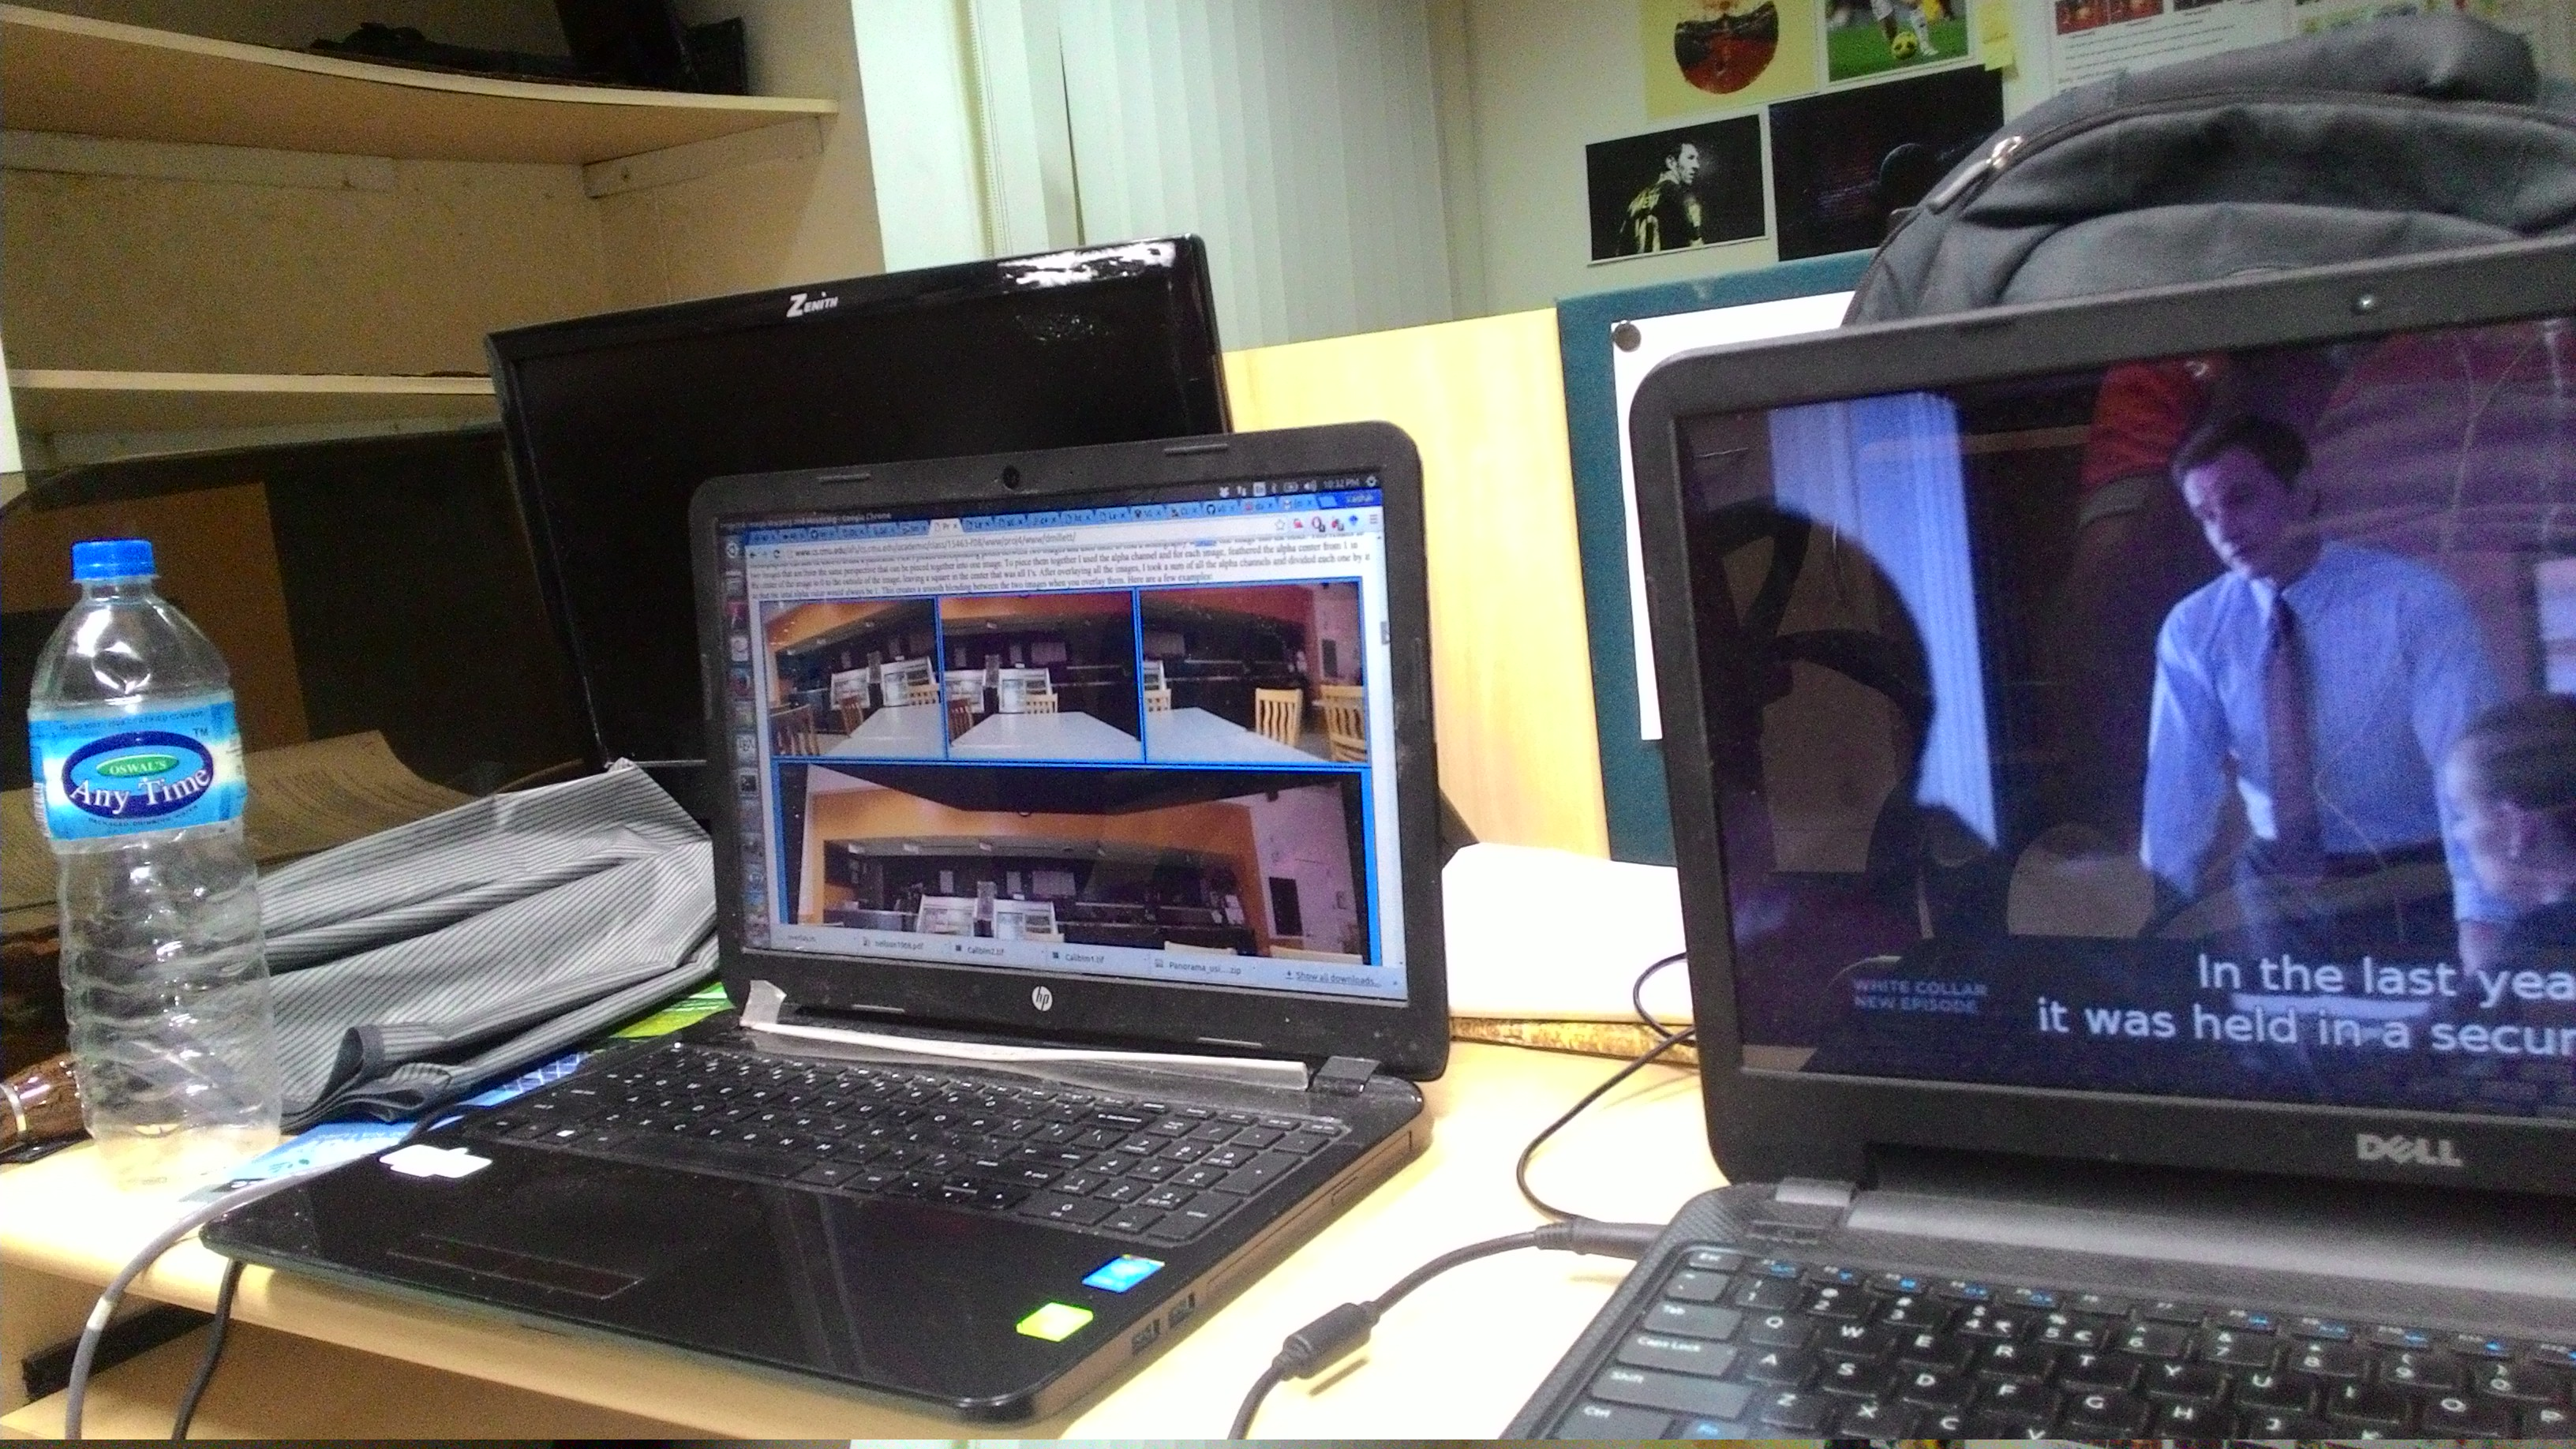
\includegraphics[scale = 0.067]{pt1.jpg}
\caption{Image 1}
\label{fig:Image 1}
\end{minipage}%
\begin{minipage}{.5\textwidth}
\centering
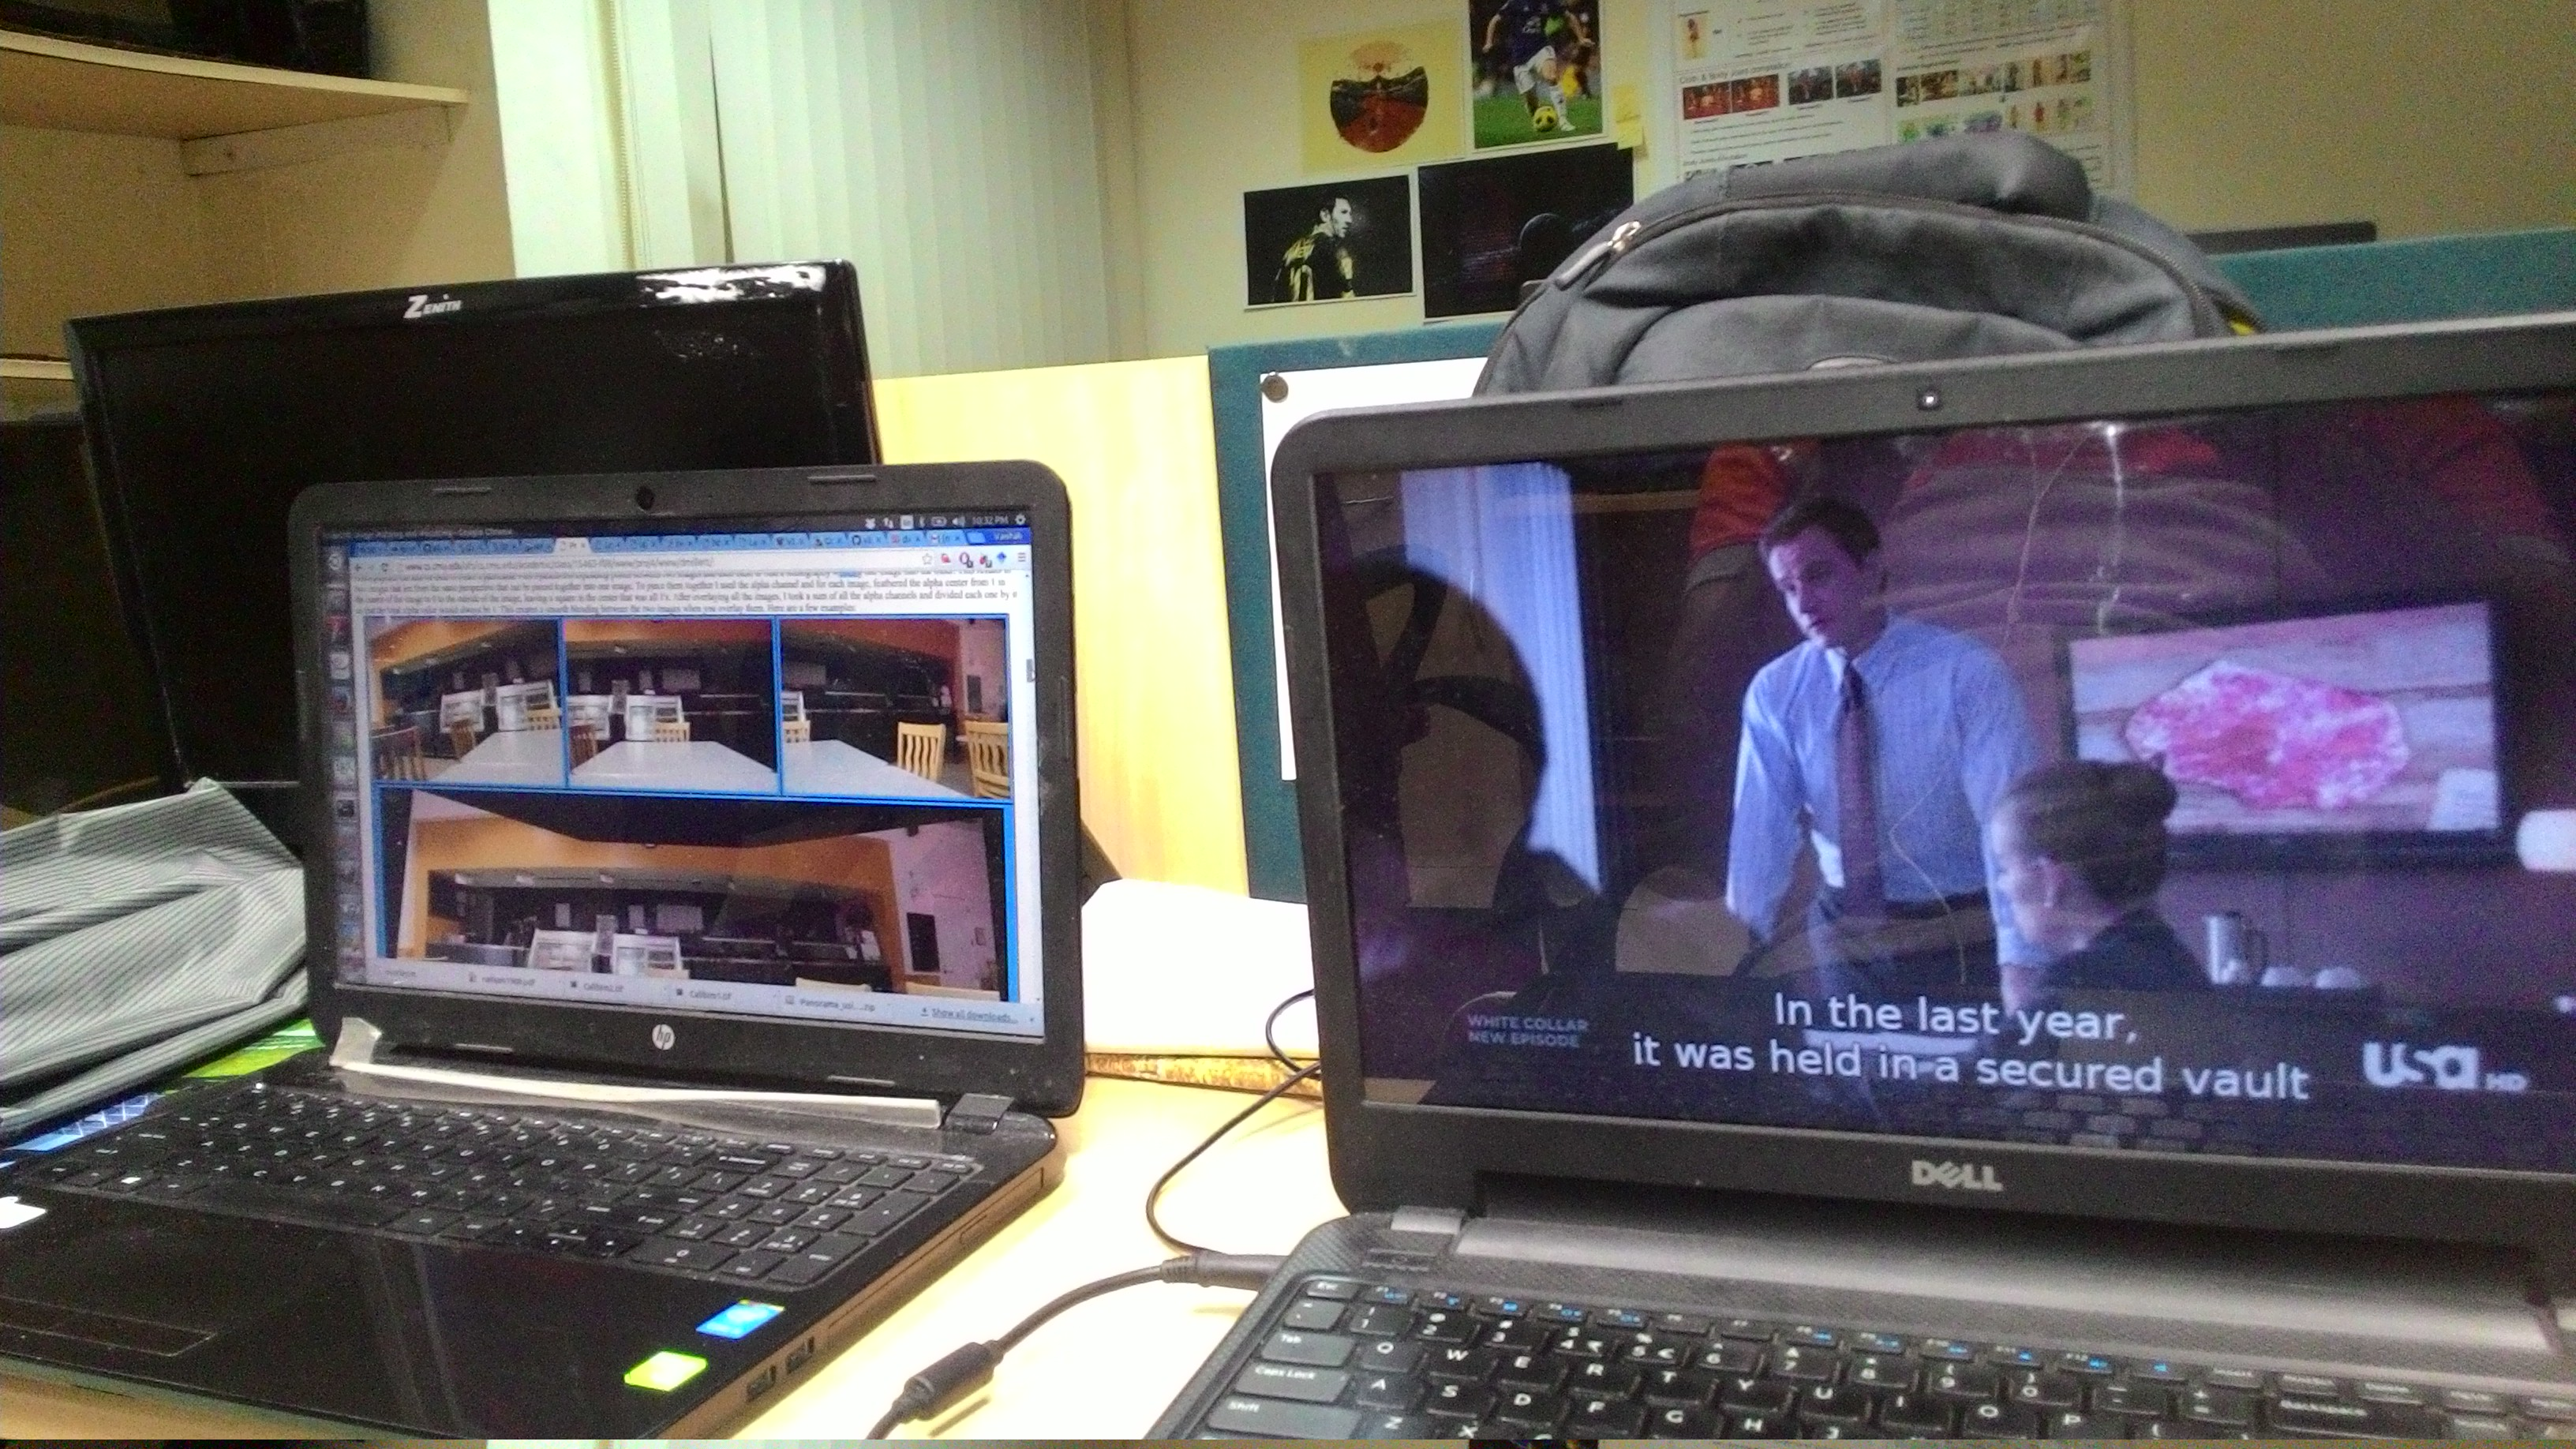
\includegraphics[scale = 0.067]{pt2.jpg}
\caption{Image 2}
\label{fig:Image 2}
\end{minipage}%
\end{figure}
\clearpage

\subsection{Output}

The parameters of the camera matrix are as follows:
\subsubsection{Camera Projection Matrix, P} 
\begin{tabular}{|c|c|c|}
\hline

  1.2534 &  -0.046 &  -337.3064  \\ 
 0.1076 &  1.1222 &  -60.9532  \\ 
 0.0002 &  0 &  1  \\ 

\hline
\end{tabular}
             
    
\subsubsection{Intrinsic Parameters, K}
\begin{tabular}{|c|c|c|}
\hline

 -1.3102 &  -0.0824 &  -337.3062 \\
 0 &  -1.1267 &  -60.9532 \\
 0 &  0 &  1 \\

\hline
\end{tabular}


\subsubsection{Rotation Matrix}
\begin{tabular}{|c|c|c|}
\hline

  -0.9945 &  0.1048 &  0.0002 \\
 -0.1048 &  -0.9945 &  0 \\
 0.0002 &  0 &  1 \\
\hline
\end{tabular}
         

\subsubsection{Center of Camera}
\begin{tabular}{|c|c|c|}
\hline

 0  &  0 &  1.0000 \\ 
  \hline
\end{tabular}



\subsubsection{Output Image}
The matched points of SIFT are shown in figure \ref{sift} and the estimated points from the homography matrix is shown in the figure \ref{ransacsift}
\begin{figure}[htp]
\centering
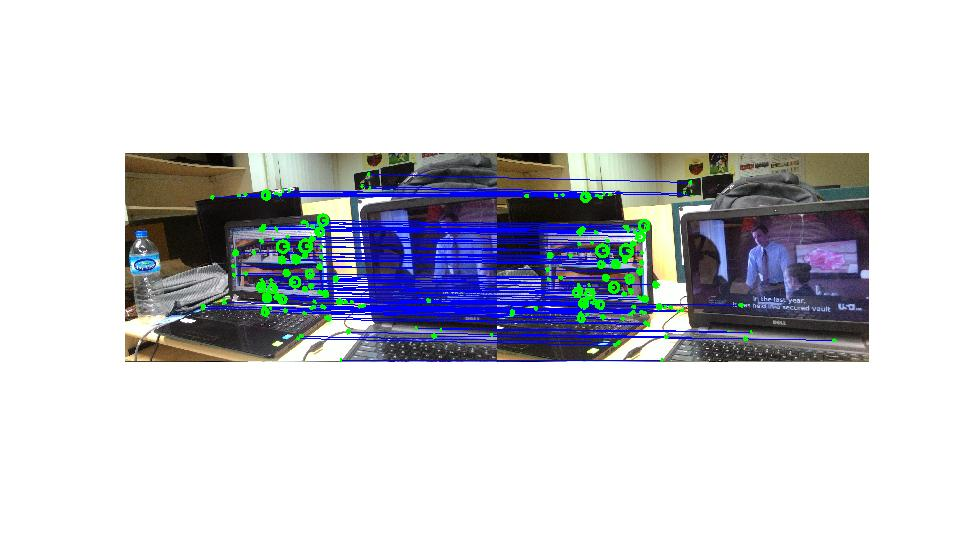
\includegraphics[width=1\textwidth]{siftPt.jpg}\hfill
\label{sift}
\caption{Matched points from SIFT}
\end{figure}

\begin{figure}[htp]
\centering
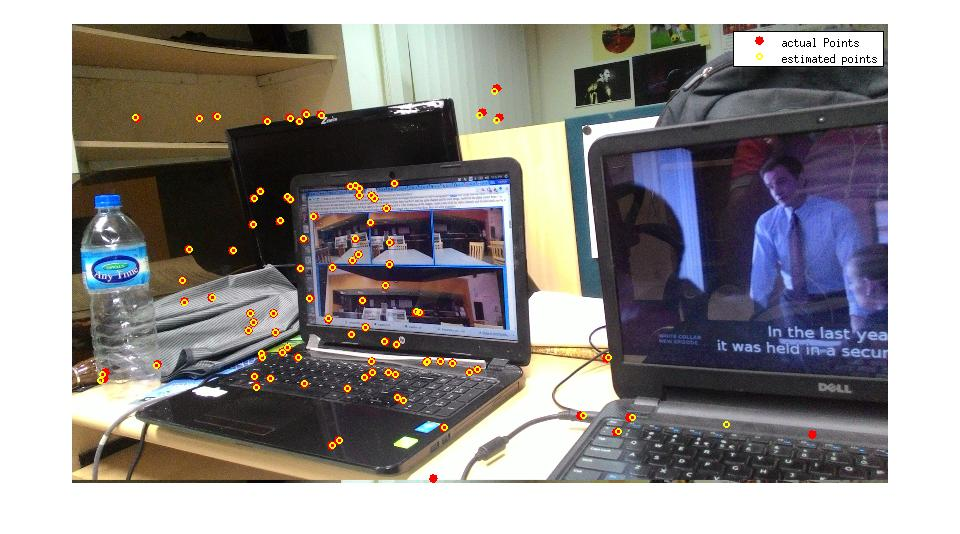
\includegraphics[width=1\textwidth]{ransacPtsift.jpg}\hfill
\label{ransacsift}
\caption{Estimated Poinsts from Homography}
\end{figure}

\clearpage
\subsubsection{Observation}
It has been observed that the image center varies in the estimated homography matrices vary significantly for manual features and SIFT identified features. The other parameters like focal lengths and skew have a difference of around 0.3. 

\section{Image Stitching with Camera at Same Location}
Image stitching or photo stitching is the process of combining multiple photographic images with overlapping fields of view to produce a segmented panorama or high-resolution image. For the experiment, image stitching has been performed by rotating the camera held at the same location.

\subsection{Code}
\begin{lstlisting}
close all;
clear all;

Ia = imread('pt1.jpg');
Ib = imread('pt2.jpg');
[im1Pts, im2Pts, Ia, Ib] = sift(Ia, Ib);

im1Pts = [im1Pts; ones(1, size(im1Pts,2))];
im1Pts = im1Pts';
im2Pts = [im2Pts; ones(1, size(im2Pts,2))];
im2Pts = im2Pts';
size(im1Pts)
size(im2Pts)
[p, K, R, C, imgEstimated] = ransac(im2Pts, im1Pts, Ib, Ia);

im1 = Ia;
im2 = Ib;
p = p/p(3,3);
H=maketform('projective',p');

[im2t,xdim2t,ydim2t]=imtransform(im1,T);
xRange=[min(1,xdim2t(1)) max(size(im2,2),xdim2t(2))];
yRange=[min(1,ydim2t(1)) max(size(im2,1),ydim2t(2))];

im2t=imtransform(im1,H,'XData',xRange,'YData',yRange);
im1t=imtransform(im2,maketform('affine',eye(3)),
'XData',xRange,'YData',yRange);

ims=max(im1t,im2t);
figure;
imshow(ims);



Ic = imread('pt3.jpg');
[im1Pts, im2Pts, Ib, Ic] = sift(Ib, Ic);

im1Pts = [im1Pts; ones(1, size(im1Pts,2))];
im1Pts = im1Pts';
im2Pts = [im2Pts; ones(1, size(im2Pts,2))];
im2Pts = im2Pts';
size(im1Pts)
size(im2Pts)
[p, K, R, C, imgEstimated] = ransac(im2Pts, im1Pts, Ic, Ib);

im1 = Ib;
im2 = Ic;
p = p/p(3,3);
T=maketform('projective',p');

[im2t,xdataim2t,ydataim2t]=imtransform(im1,T);
%now xdataim2t and ydataim2t store the bounds of the transformed im2
xdataout=[min(1,xdataim2t(1)) max(size(im2,2),xdataim2t(2))];
ydataout=[min(1,ydataim2t(1)) max(size(im2,1),ydataim2t(2))];

im2t=imtransform(im1,T,'XData',xdataout,'YData',ydataout);
im1t=imtransform(im2,maketform('affine',eye(3)),'XData',xdataout,
'YData',ydataout);
 
figure;
imshow(im2t);
figure;
imshow(im1t);

im2t = imresize(im2t, [size(im1t,1), size(im1t,2)]);

ims3=max(im1t,im2t);
figure;
imshow(ims);

figure;
imshow(ims3);


[im1Pts, im2Pts, ims, ims3] = sift(ims, ims3);

im1Pts = [im1Pts; ones(1, size(im1Pts,2))];
im1Pts = im1Pts';
im2Pts = [im2Pts; ones(1, size(im2Pts,2))];
im2Pts = im2Pts';
size(im1Pts)
size(im2Pts)
[p, K, R, C, imgEstimated] = ransac(im2Pts, im1Pts, ims3, ims);

im1 = ims;
im2 = ims3;
p = p/p(3,3);
T=maketform('projective',p');

[im2t,xdim2t,ydim2t]=imtransform(im1,T);
xRange=[min(1,xdim2t(1)) max(size(im2,2),xdim2t(2))];
yRange=[min(1,ydim2t(1)) max(size(im2,1),ydim2t(2))];
im2t=imtransform(im1,T,'XData',xRange,'YData',yRange);
im1t=imtransform(im2,maketform('affine',eye(3)),'XData',xRange,
'YData',yRange);

ims4=max(im1t,im2t);
figure;
imshow(ims4);
\end{lstlisting}

\subsection{Input}
Two sets of images have been used in the experiment. One set is of laptops on a desk, the other set is of a room.
\begin{figure}[h]
\centering
\begin{minipage}{0.6\textwidth}
\centering
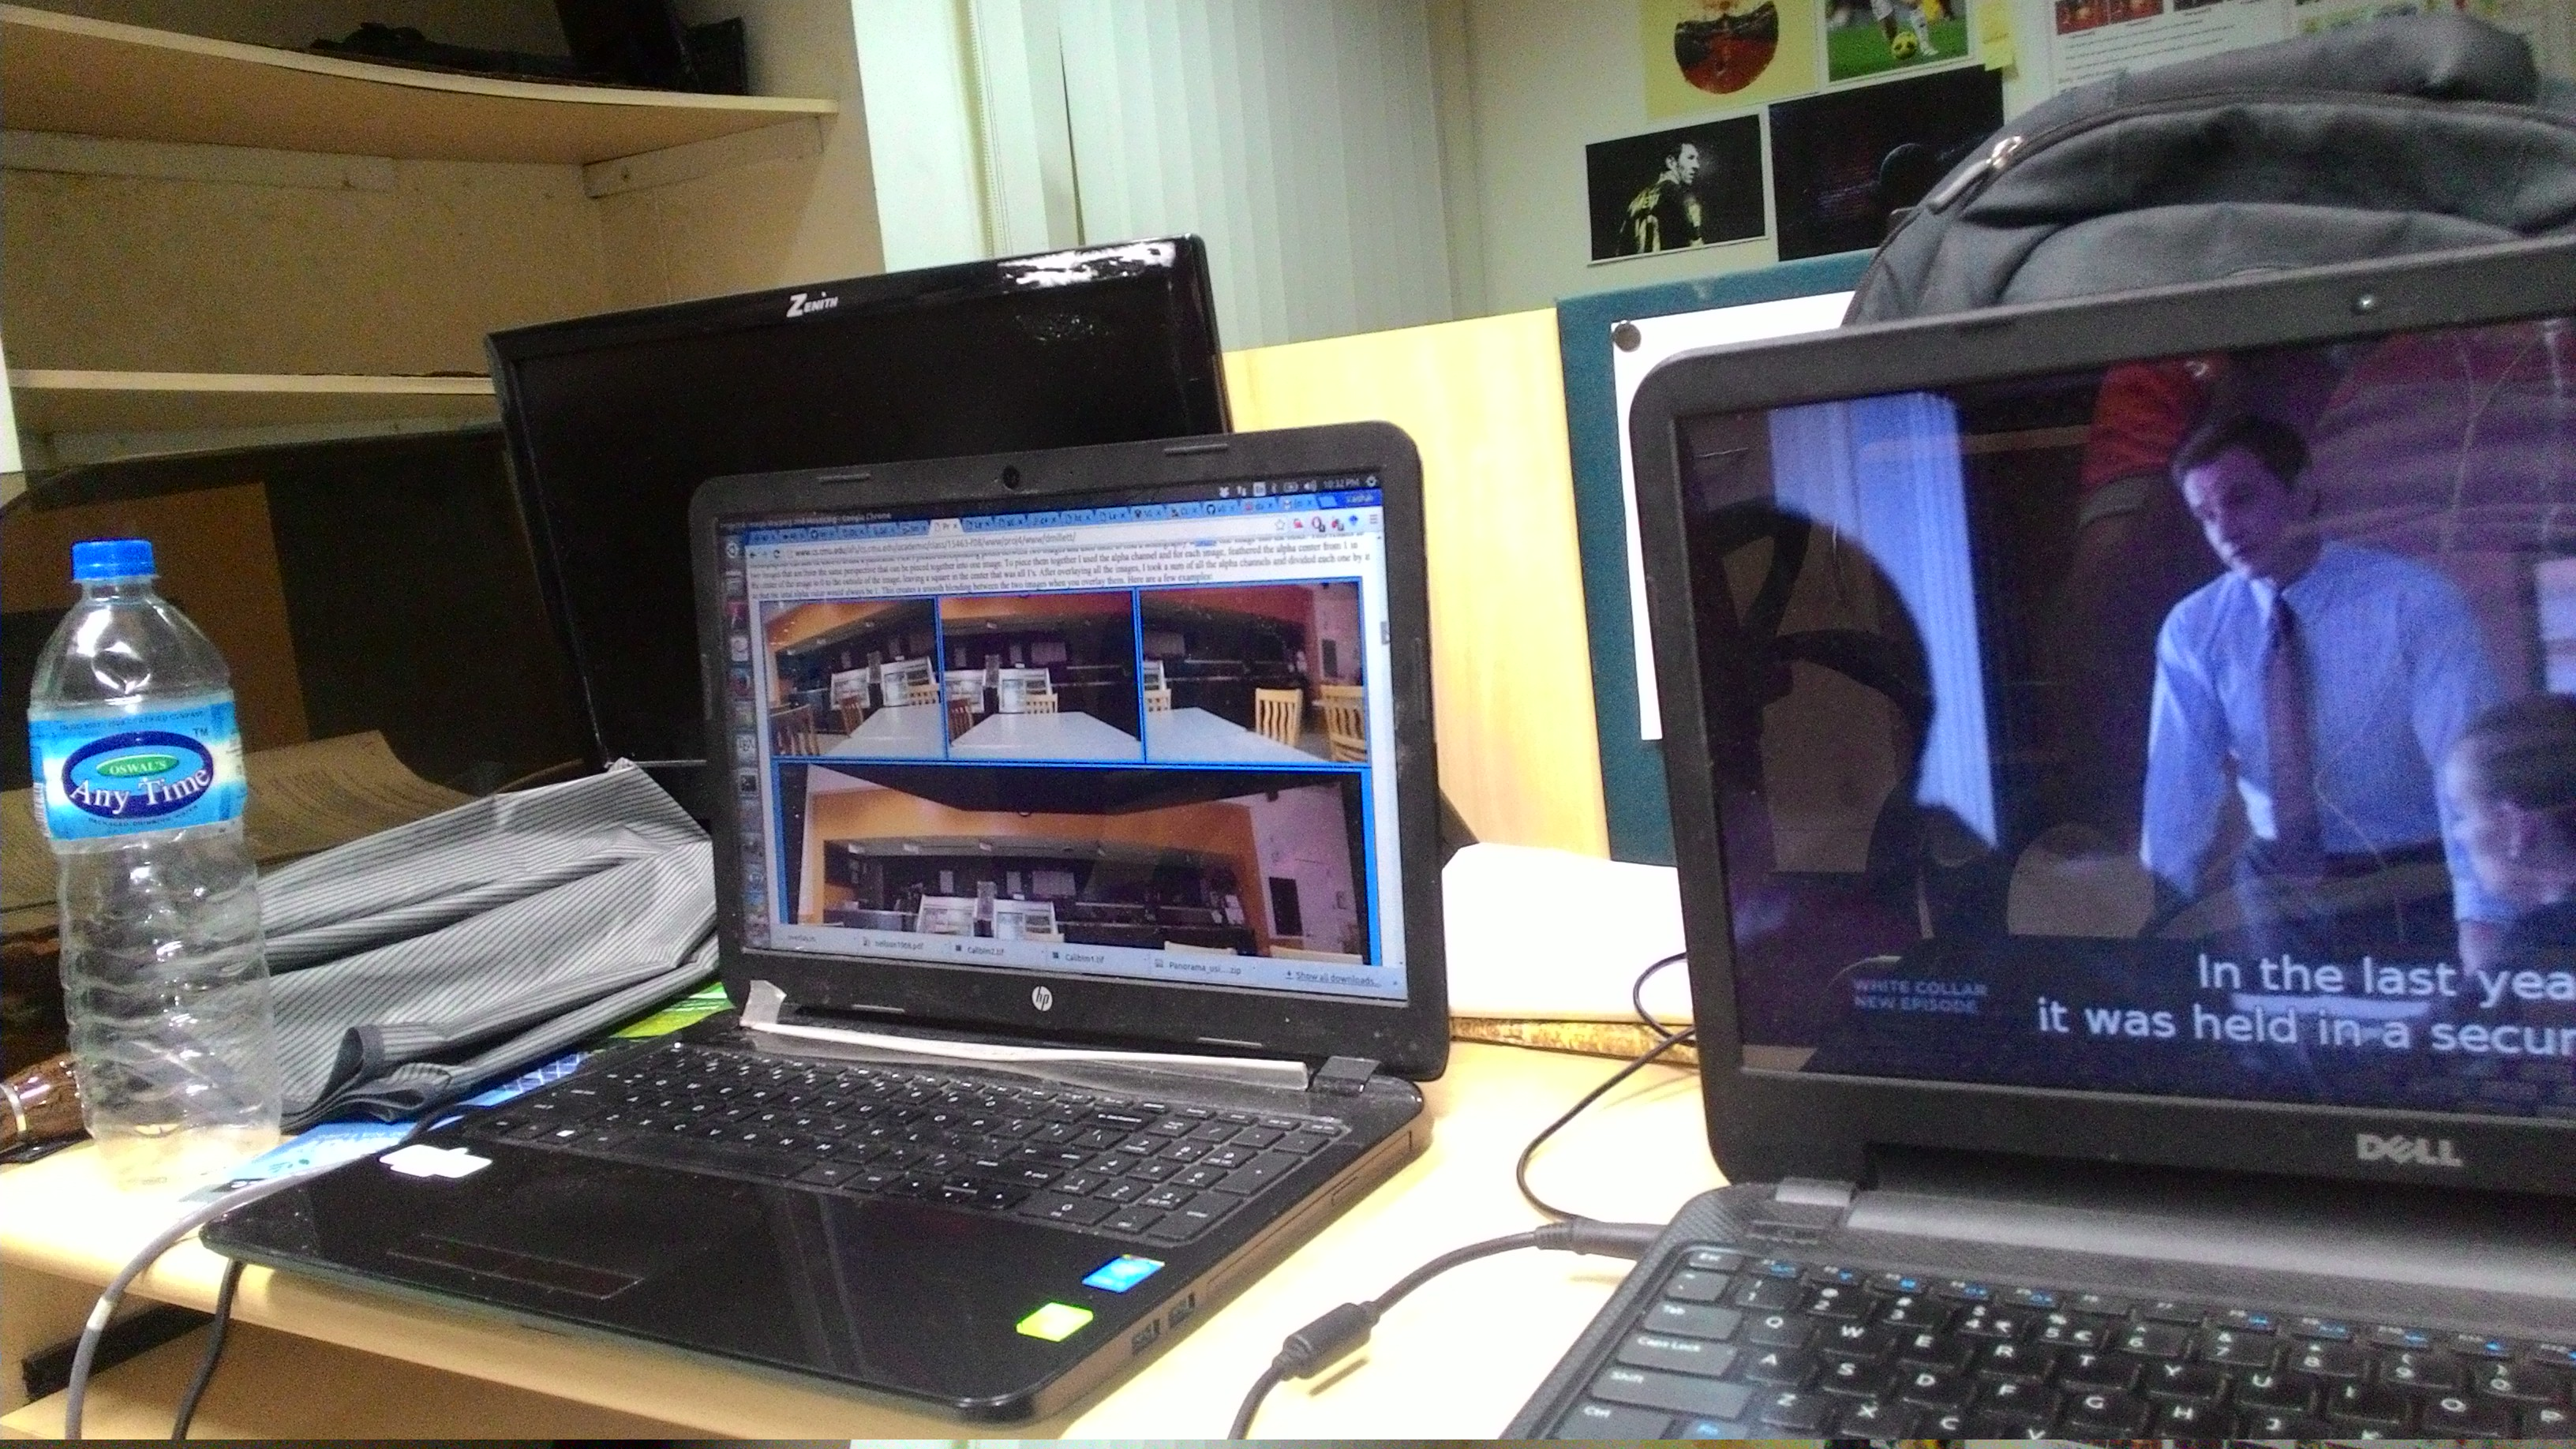
\includegraphics[scale = 0.067]{pt1.jpg}
\caption{Image 1}
\label{fig:Image 1}
\end{minipage}%
\begin{minipage}{.5\textwidth}
\centering
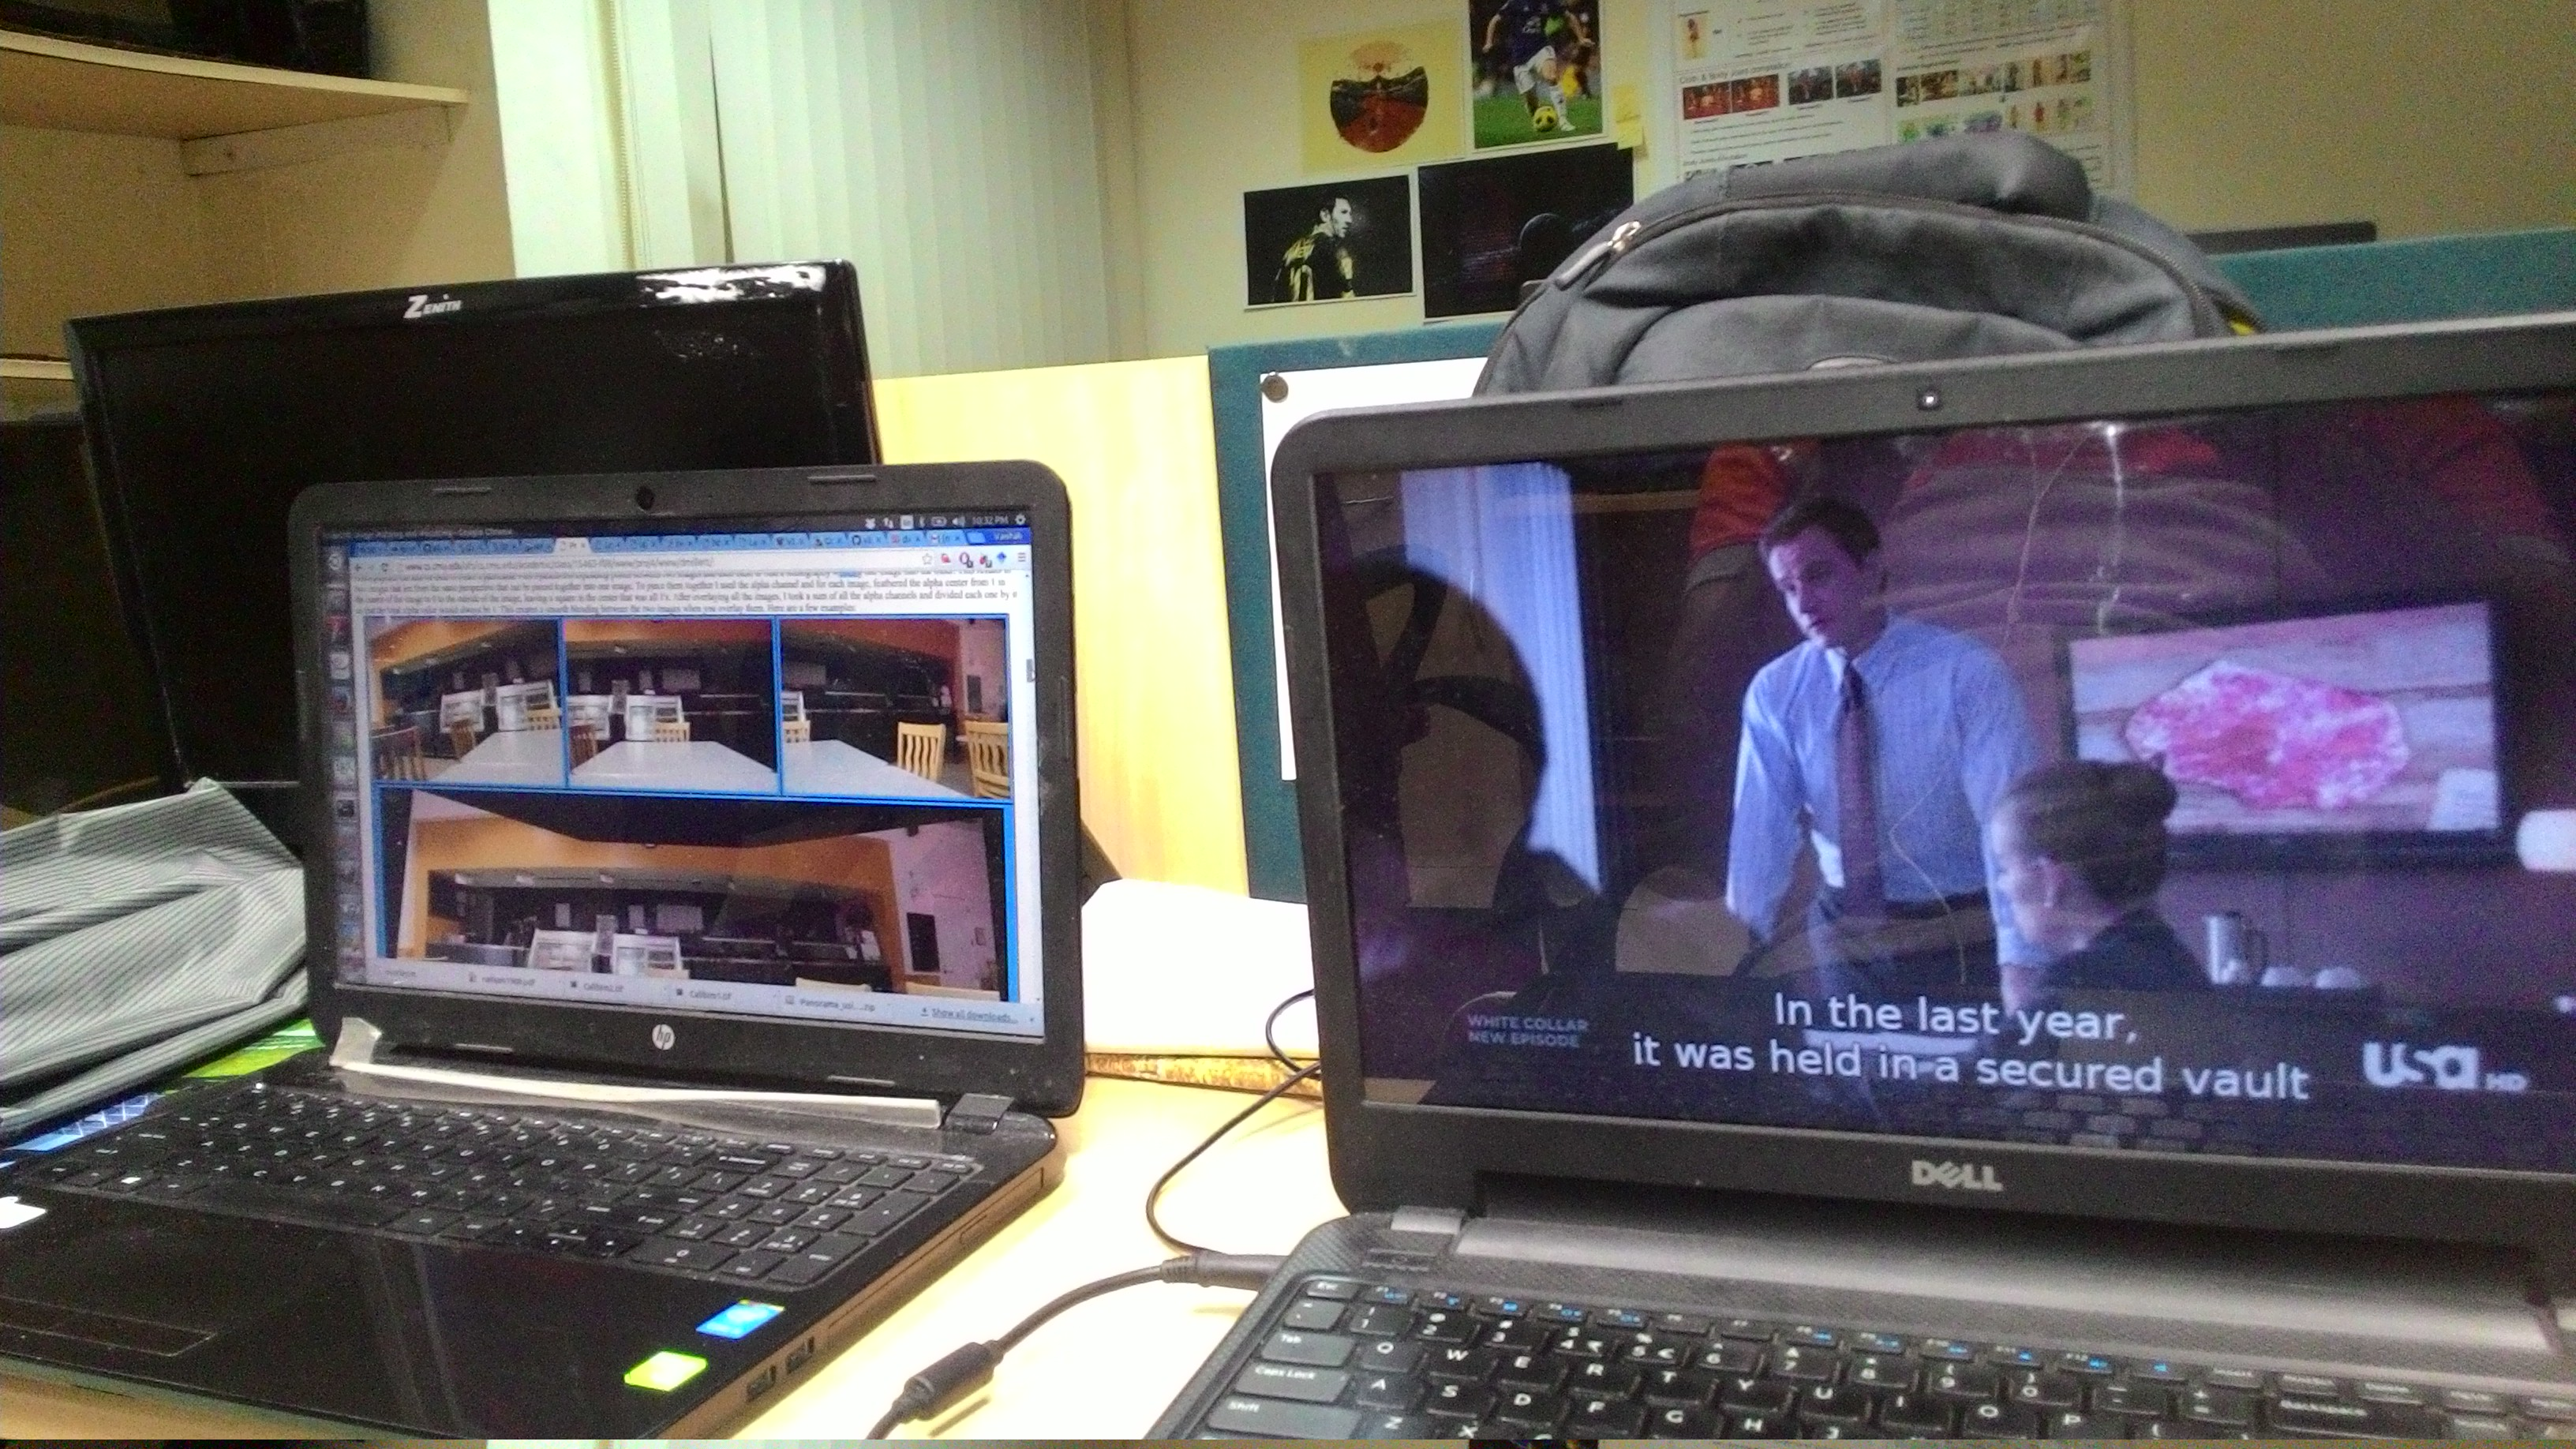
\includegraphics[scale = 0.067]{pt2.jpg}
\caption{Image 2}
\label{fig:Image 2}
\end{minipage}%
\end{figure}

\begin{figure}[htp]
\centering
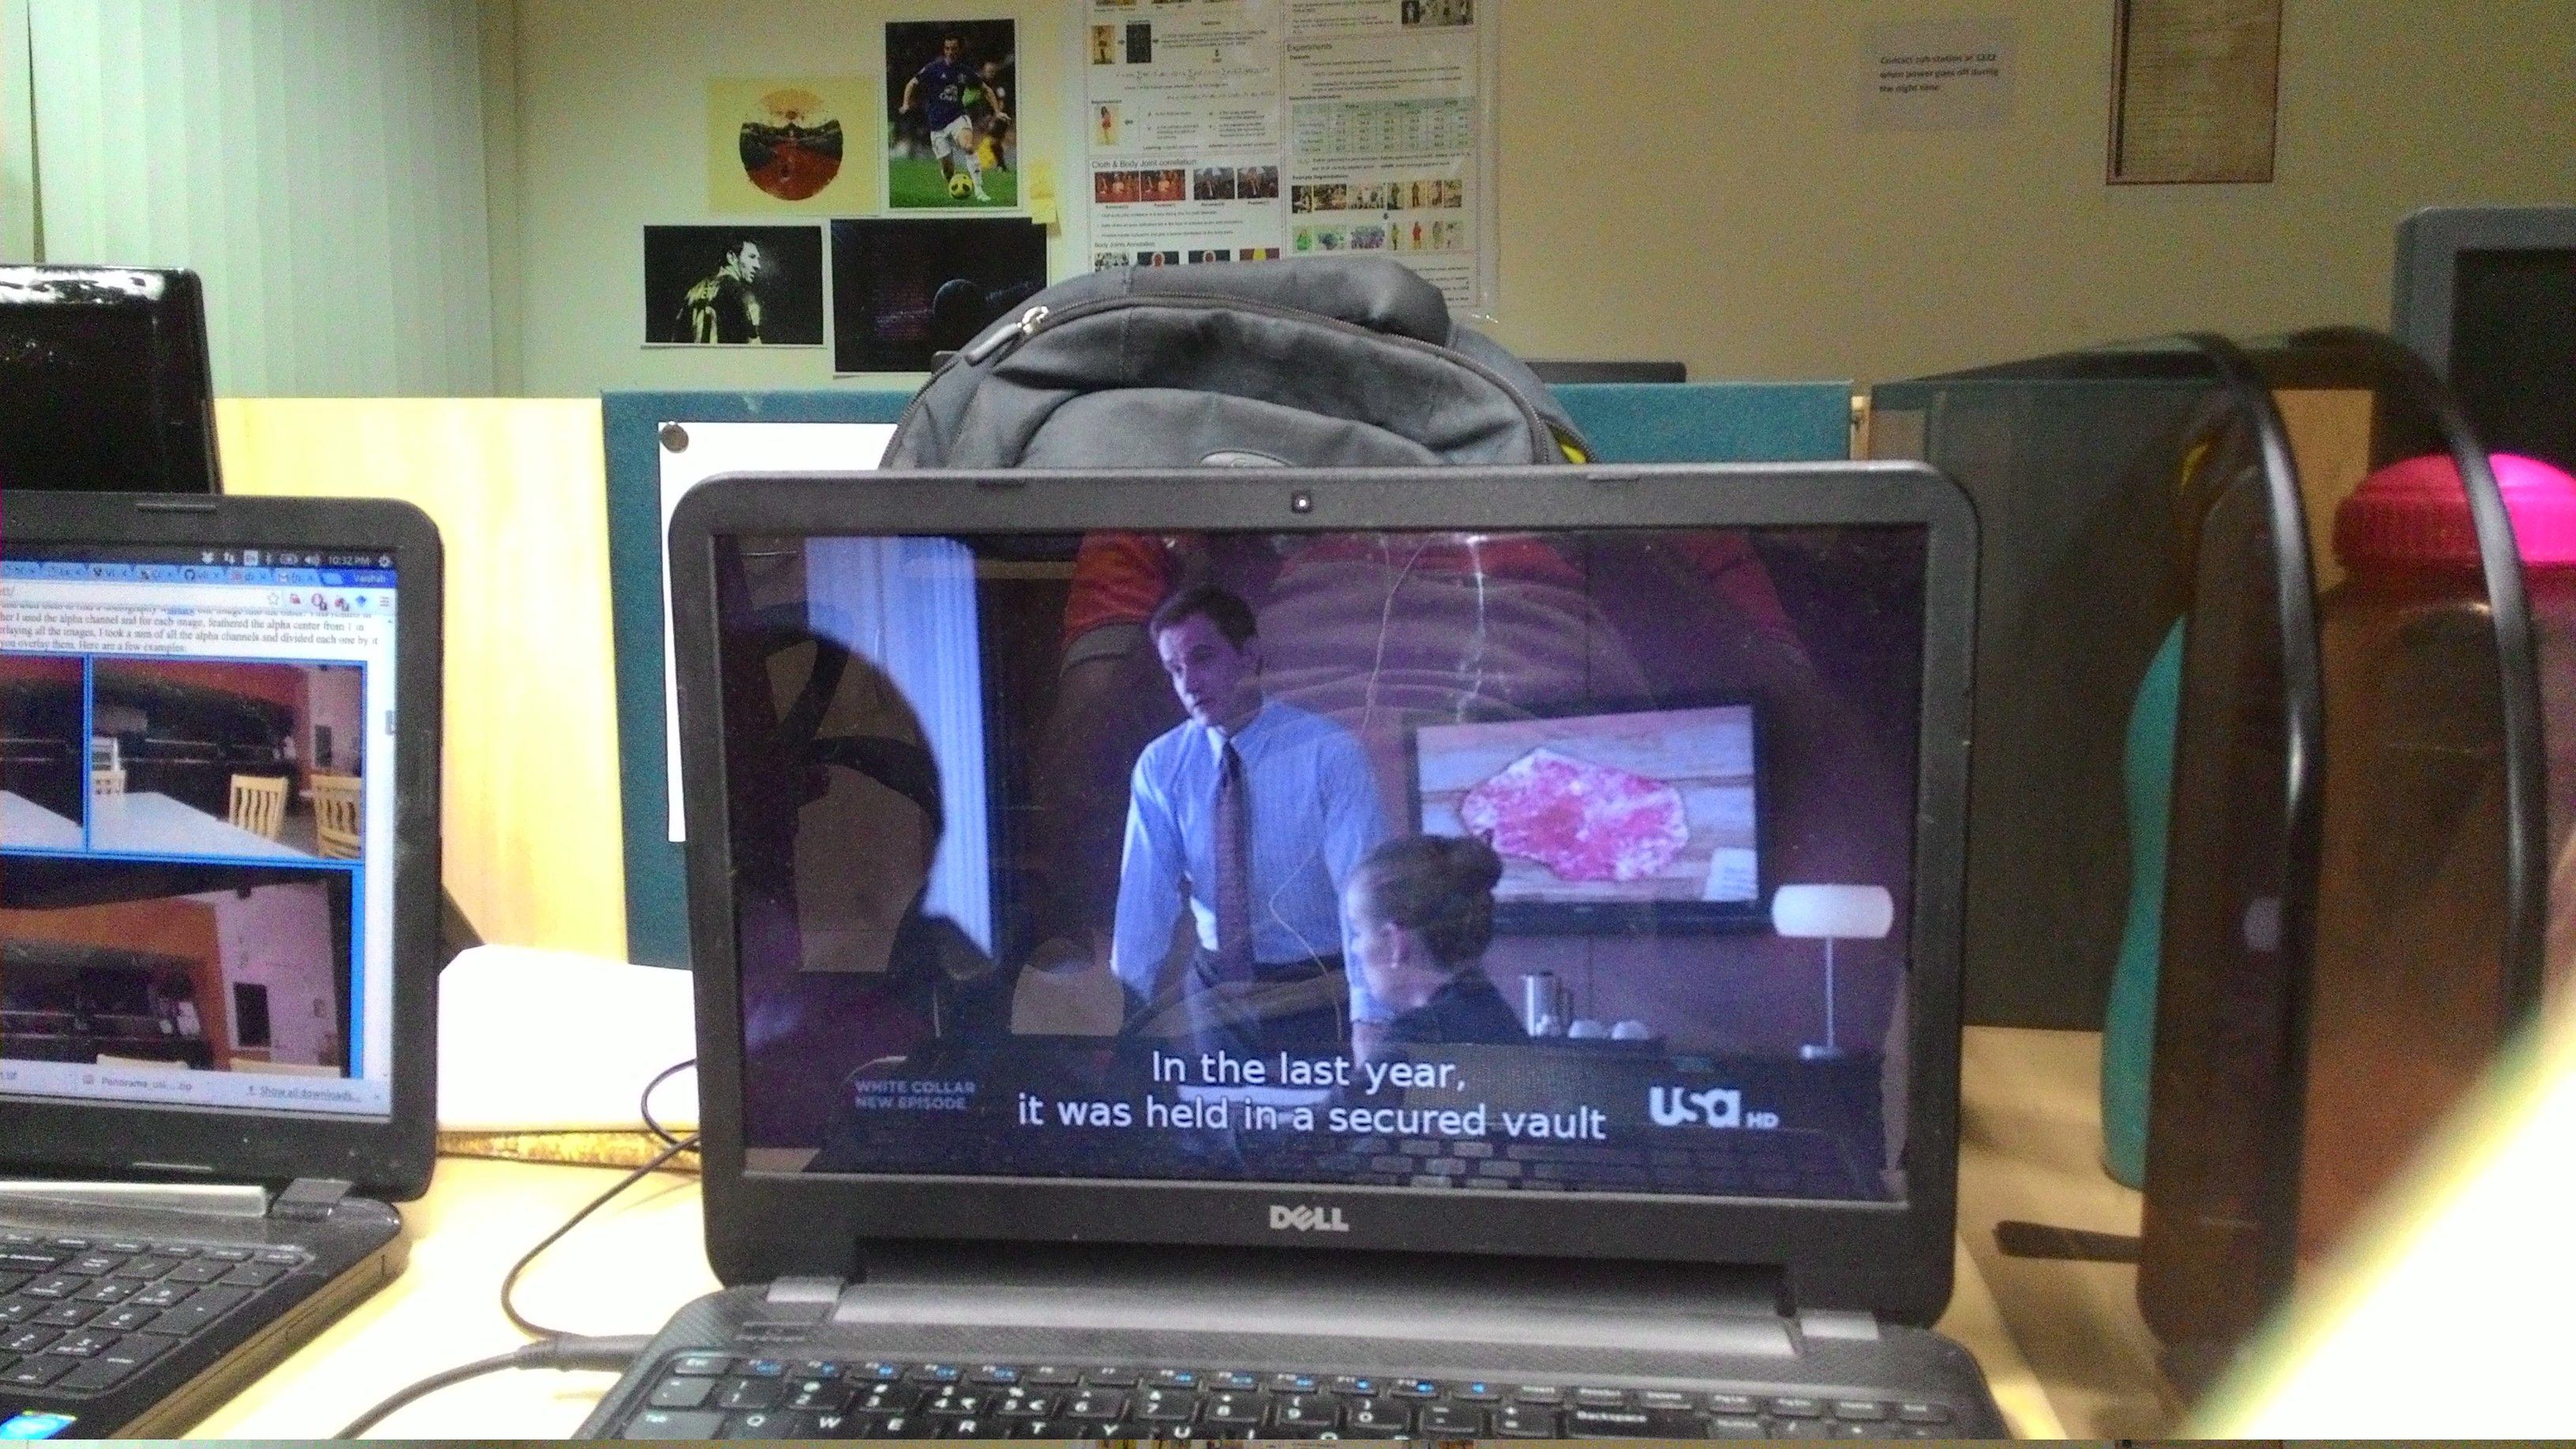
\includegraphics[width=0.57\textwidth]{pt3.jpg}\hfill
\caption{Image 3}
\end{figure}
\clearpage


\begin{figure}[h]
\centering
\begin{minipage}{0.6\textwidth}
\centering
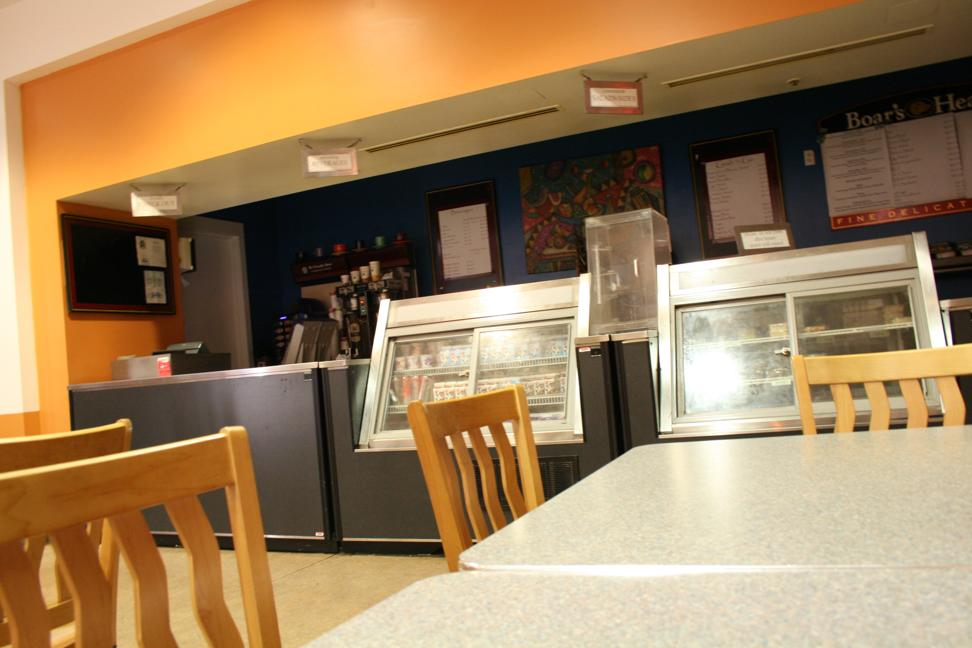
\includegraphics[scale = 0.2]{test5.jpg}
\caption{Image 1}
\label{fig:Image 1}
\end{minipage}%
\begin{minipage}{.5\textwidth}
\centering
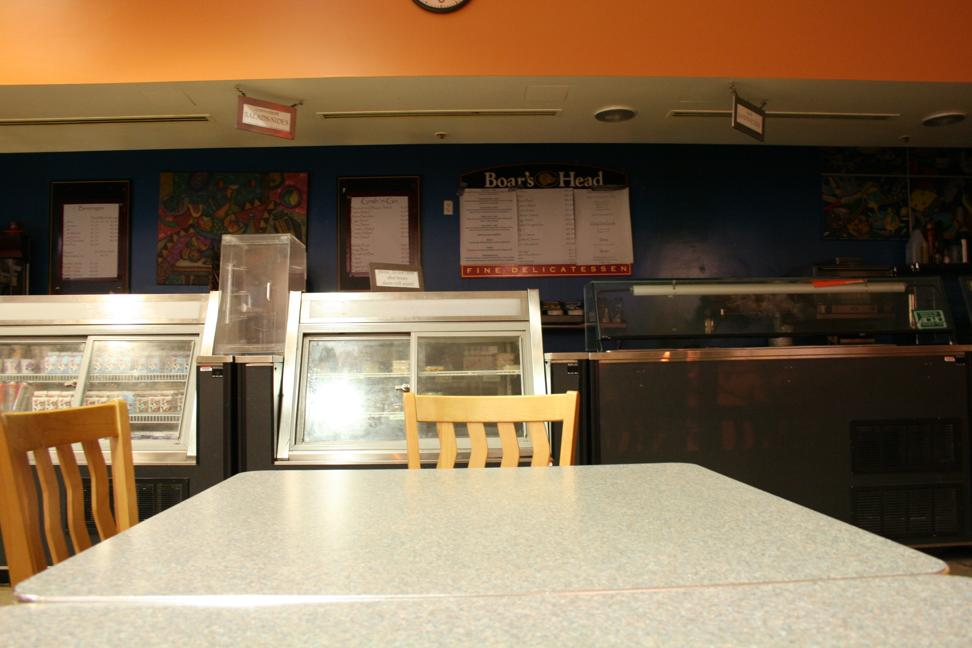
\includegraphics[scale = 0.2]{test6.jpg}
\caption{Image 2}
\label{fig:Image 2}
\end{minipage}%
\end{figure}

\begin{figure}[htp]
\centering
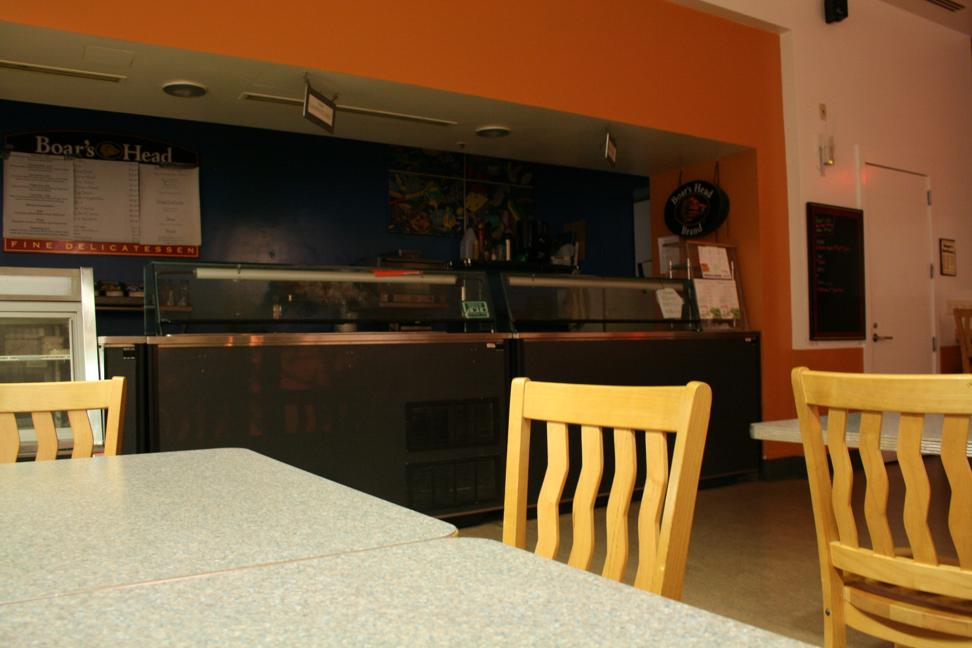
\includegraphics[width=0.5\textwidth]{test7.jpg}\hfill
\caption{Image 3}
\end{figure}

\clearpage

\subsection{Output}
The stitched images of the 2 sets of images are as follows:

\begin{figure}[h]
\centering
\begin{minipage}{0.3\textwidth}
\centering
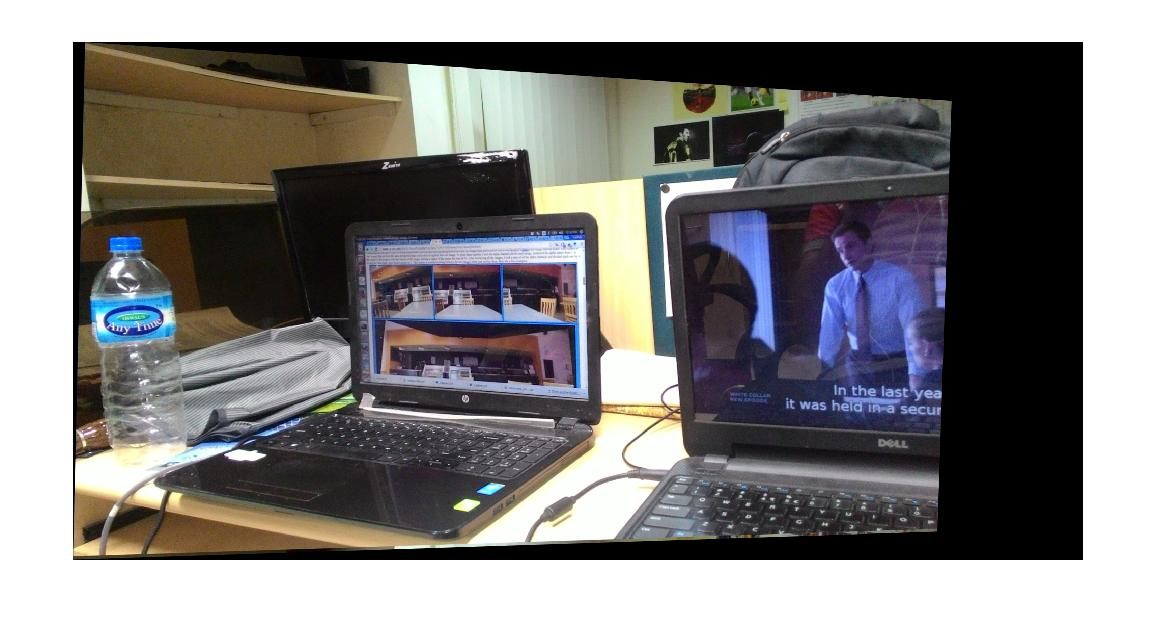
\includegraphics[scale = 0.1]{stitch1.jpg}
\caption{Image 1}
\label{fig:Image 1}
\end{minipage}%
\begin{minipage}{.3\textwidth}
\centering
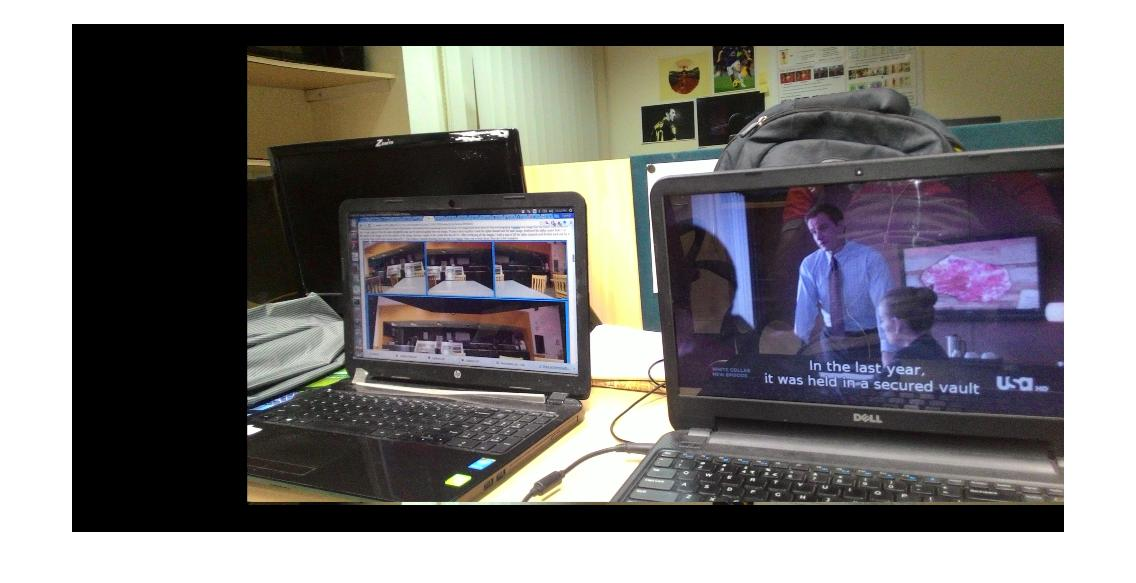
\includegraphics[scale = 0.1]{stitch2.jpg}
\caption{Image 2}
\label{fig:Image 2}
\end{minipage}%
\begin{minipage}{.3\textwidth}
\centering
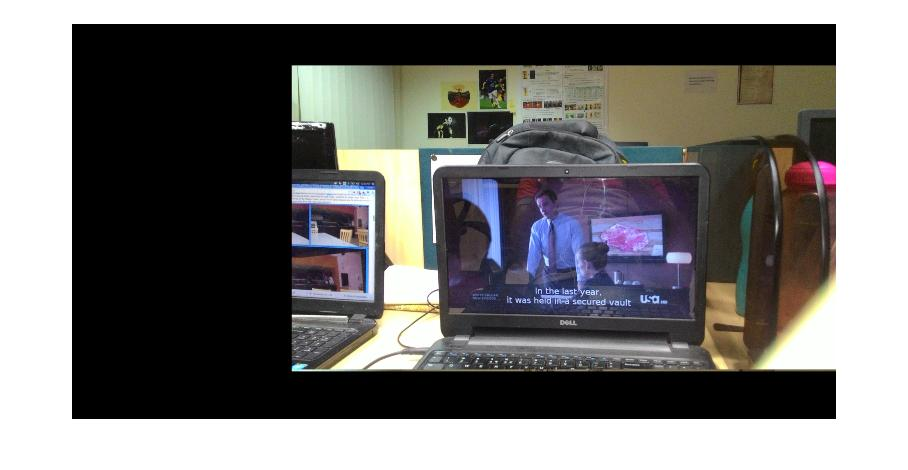
\includegraphics[scale = 0.14]{stitch3.jpg}
\caption{Image 3}
\label{fig:Image 2}
\end{minipage}%

\end{figure}


\begin{figure}[htp]
\centering
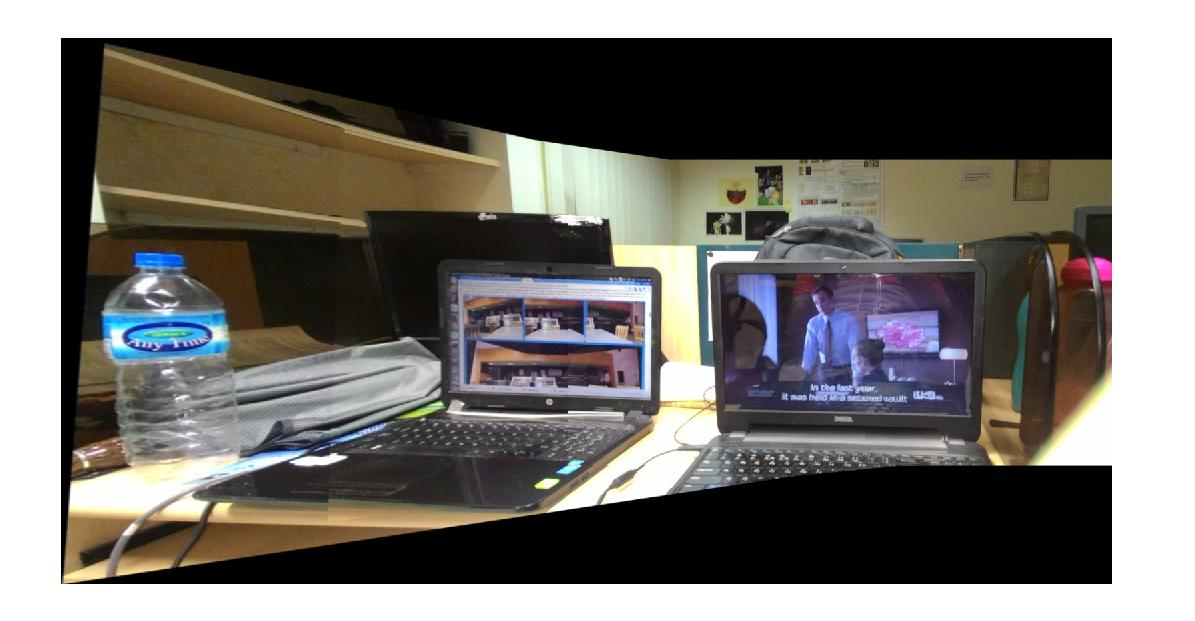
\includegraphics[width=1\textwidth]{imageStitching2.jpg}\hfill
\caption{Stitched Image}
\end{figure}



\begin{figure}[htp]
\centering
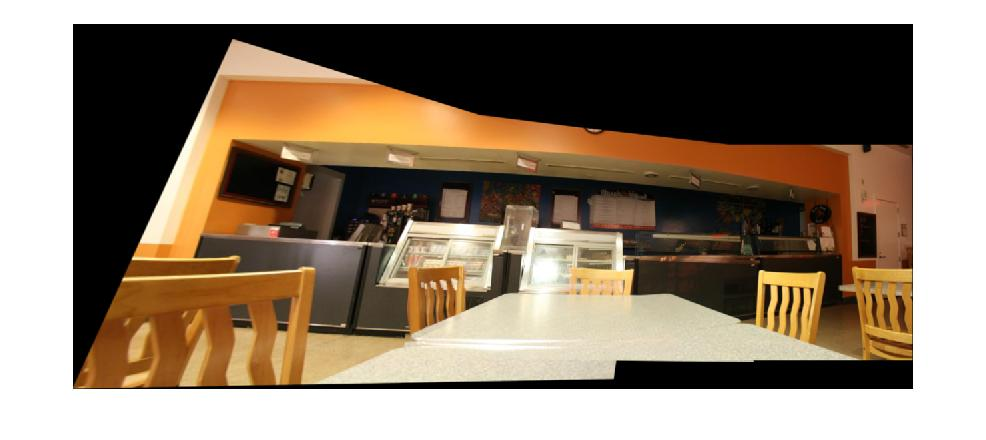
\includegraphics[width=1\textwidth]{imageSticthing1.jpg}\hfill
\end{figure}

\clearpage

\section{Image Stitching of Planar Scene}
Image stitching using homography can be done if the input images are of planar scenes. There is no restriction on the camera position or alignment in such an experiment setup.


\subsection{Code}
\begin{lstlisting}
function planarStitch()
    close all;
    clear all;
    I1 = imread('planar1.jpg');
    I2 = imread('planar2.jpg');
    I3 = imread('planar3.jpg');
    
    %% stitch image 1 and 2
    [im1Pts, im2Pts, I1, I2] = sift(I1, I2);

    im1Pts = [im1Pts; ones(1, size(im1Pts,2))]';
    im2Pts = [im2Pts; ones(1, size(im2Pts,2))]';
    [p, K, R, C, imgEstimated] = ransac(im2Pts, im1Pts, I2, I1);

    p = p/p(3,3);
    p = p';
    [im1t1, im2t1] = transform(p, I1, I2);
    ims=max(im1t1,im2t1);
    figure;
    imshow(ims);

%% stitch image 2 and 3

    [im1Pts, im2Pts, I2, I3] = sift(I2, I3);

    im1Pts = [im1Pts; ones(1, size(im1Pts,2))]';
    im2Pts = [im2Pts; ones(1, size(im2Pts,2))]';
    [p, K, R, C, imgEstimated] = ransac(im2Pts, im1Pts, I3, I2);
    p = p/p(3,3);
    p = p';
    [im1t1, im2t1] = transform(p, I2, I3);

    im2t2 = imresize(im2t2, [size(im1t2,1), size(im1t2,2)]);
    ims3=max(im1t1,im2t1);
    figure;
    imshow(ims3);

%% stitch the stitched images
    [im1Pts, im2Pts, ims, ims3] = sift(ims, ims3);
   
    im1Pts = [im1Pts; ones(1, size(im1Pts,2))]';
    im2Pts = [im2Pts; ones(1, size(im2Pts,2))]';
    [p, K, R, C, imgEstimated] = ransac(im2Pts, im1Pts, ims3, ims);
    p = p/p(3,3);
      p = p';
    [im1t, im2t] = transform(p, ims, ims3); 
    figure;
    imshow(im1t);
    figure;
    imshow(im2t);
    ims4=max(im1t,im2t);
    figure;
    imshow(ims4);
end

function [im1t, im2t] = transform(p, im1, im2)
     H=maketform('projective',p);

    [im2t,xRangeim2,yRangeim2]=imtransform(im1,H);

    xRangeF = [min(1,xRangeim2(1)) max(size(im2,2),xRangeim2(2))];
    yRangeF = [min(1,yRangeim2(1)) max(size(im2,1),yRangeim2(2))];
    im2t=imtransform(im1,H,'XData',xRangeF,'YData',yRangeF);
    im2T = maketform('affine',eye(3));
    im1t=imtransform(im2,im2T,'XData',xRangeF,'YData',yRangeF);
end
\end{lstlisting}

\subsection{Input}
The input consists of 3 images of a board on the wall.

\begin{figure}[h]
\centering
\begin{minipage}{0.7\textwidth}
\centering
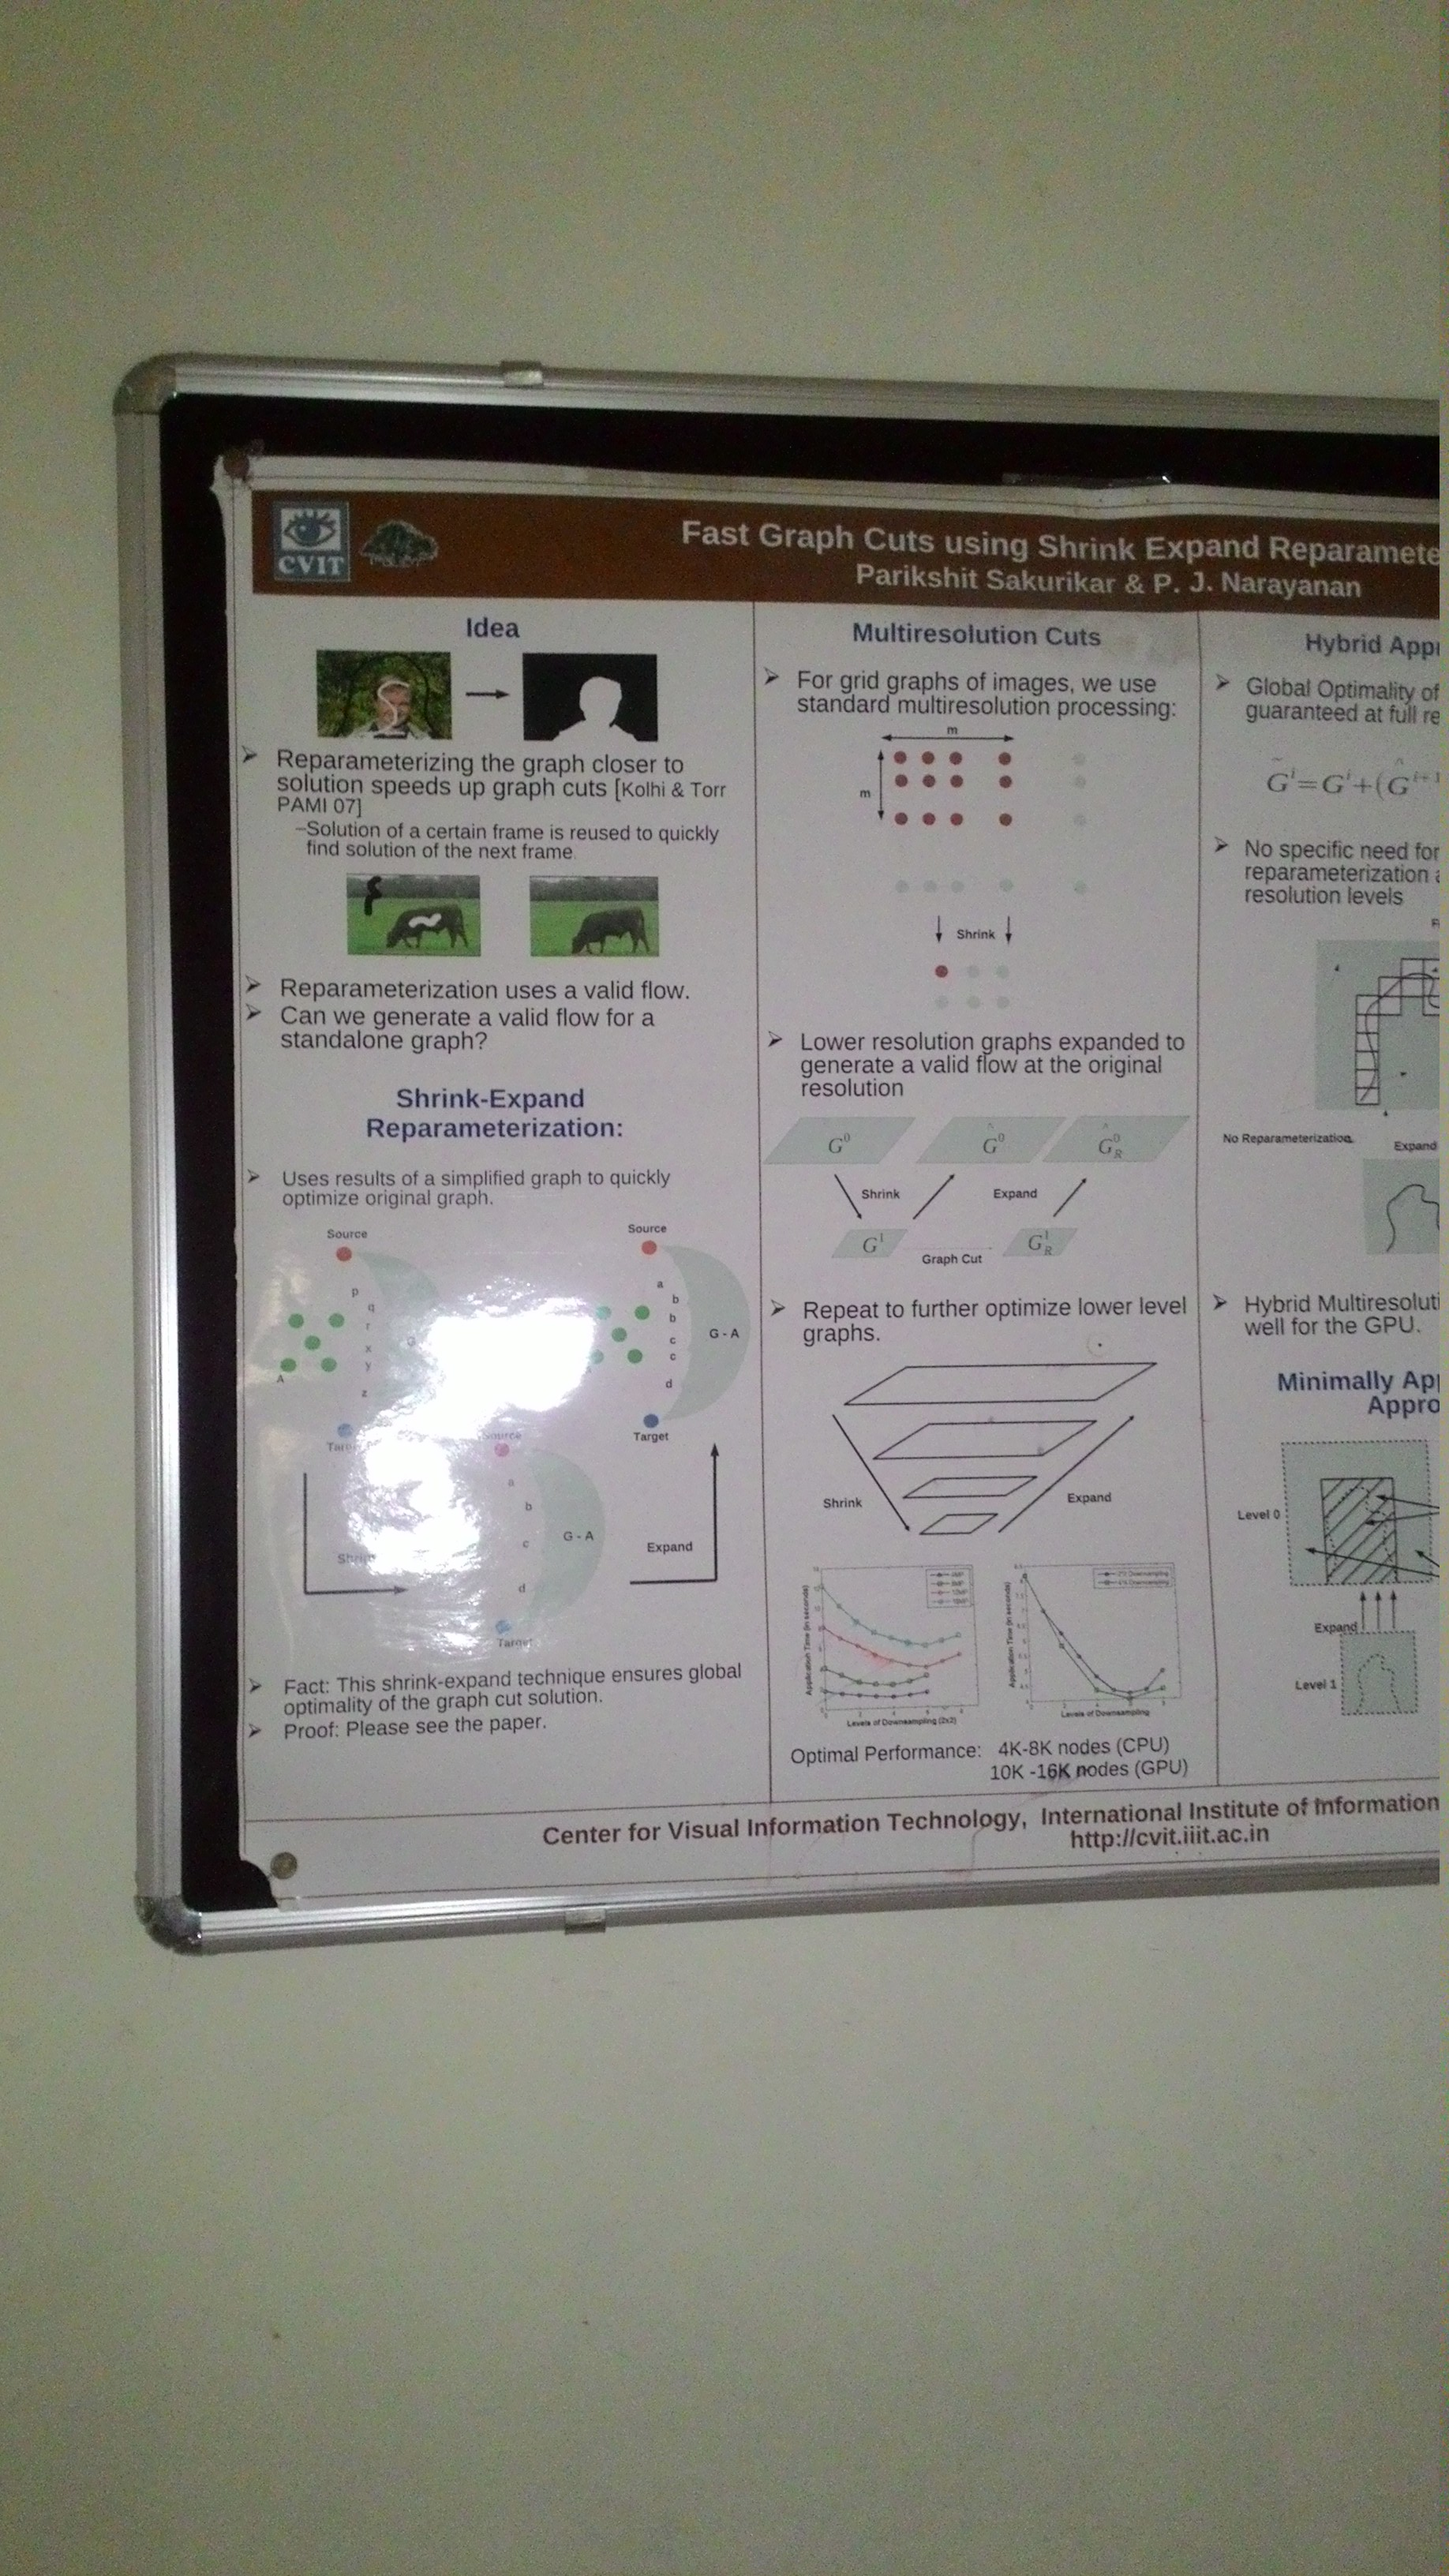
\includegraphics[scale = 0.07]{planar1.jpg}
\caption{Planar Image 1}
\label{fig:Image 1}
\end{minipage}%
\begin{minipage}{.5\textwidth}
\centering
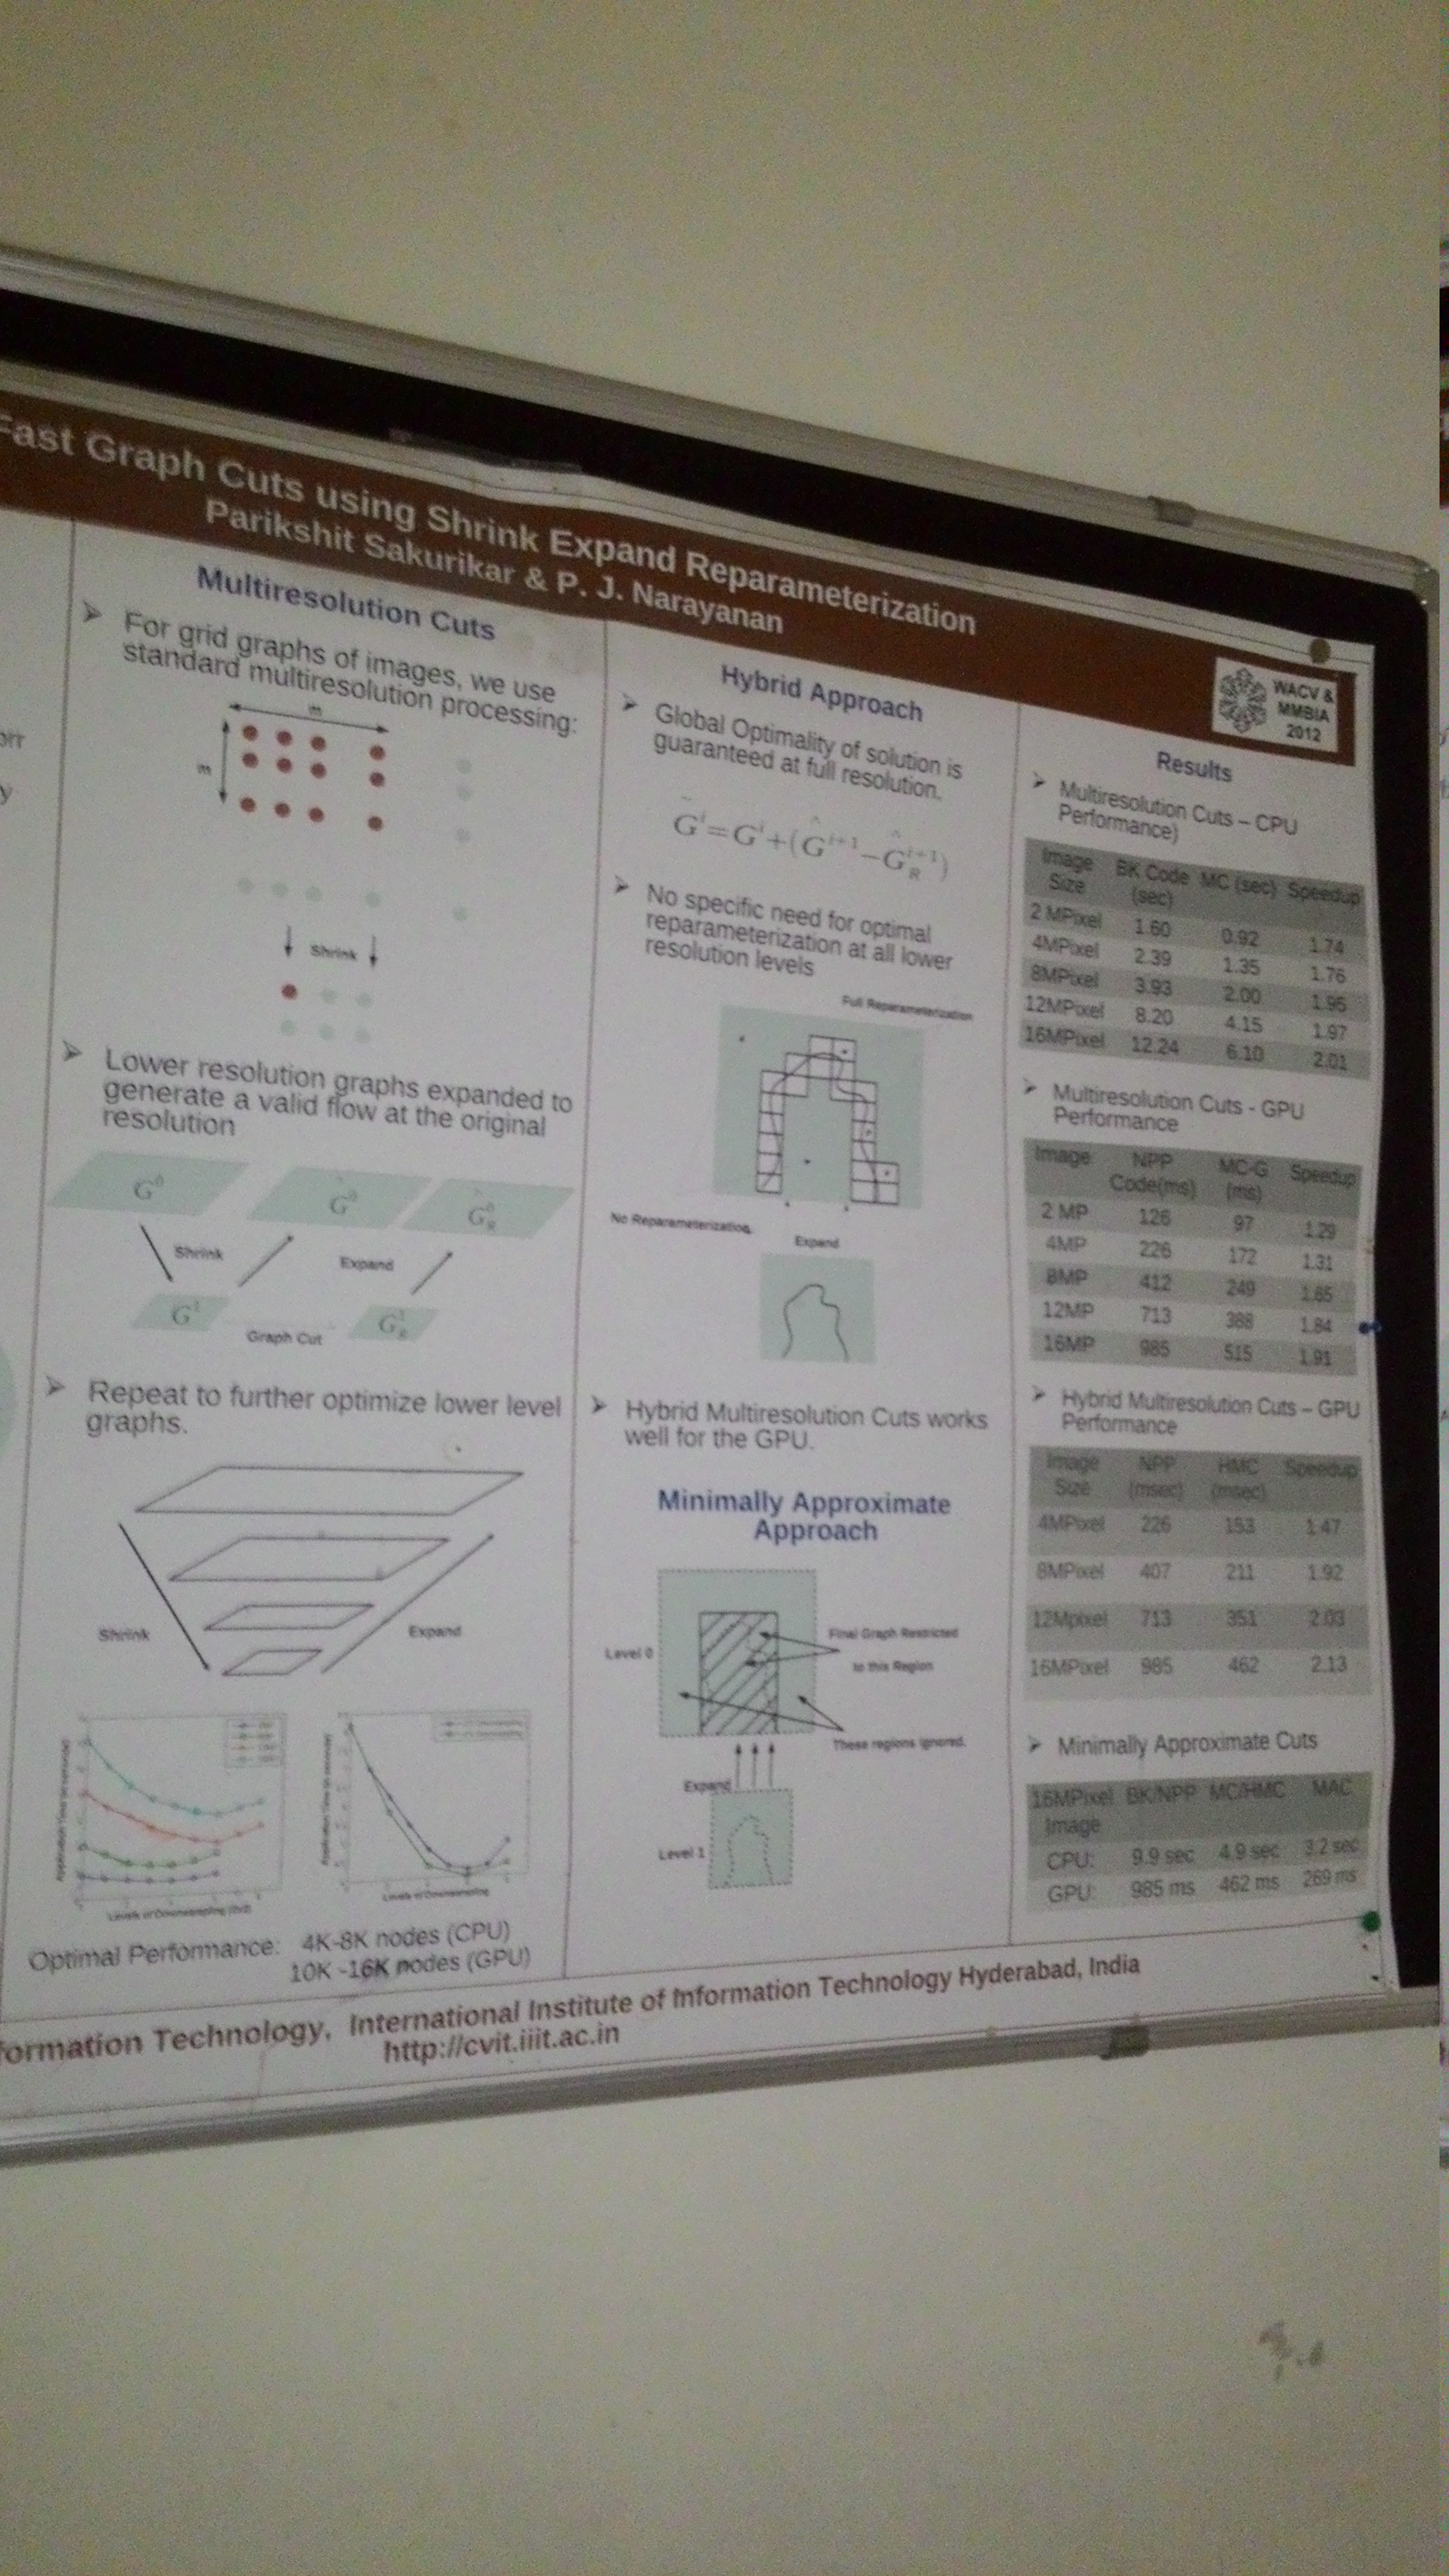
\includegraphics[scale = 0.07]{planar2.jpg}
\caption{Planar Image 2}
\label{fig:Image 2}
\end{minipage}%
\end{figure}

\begin{figure}[htp]
\centering
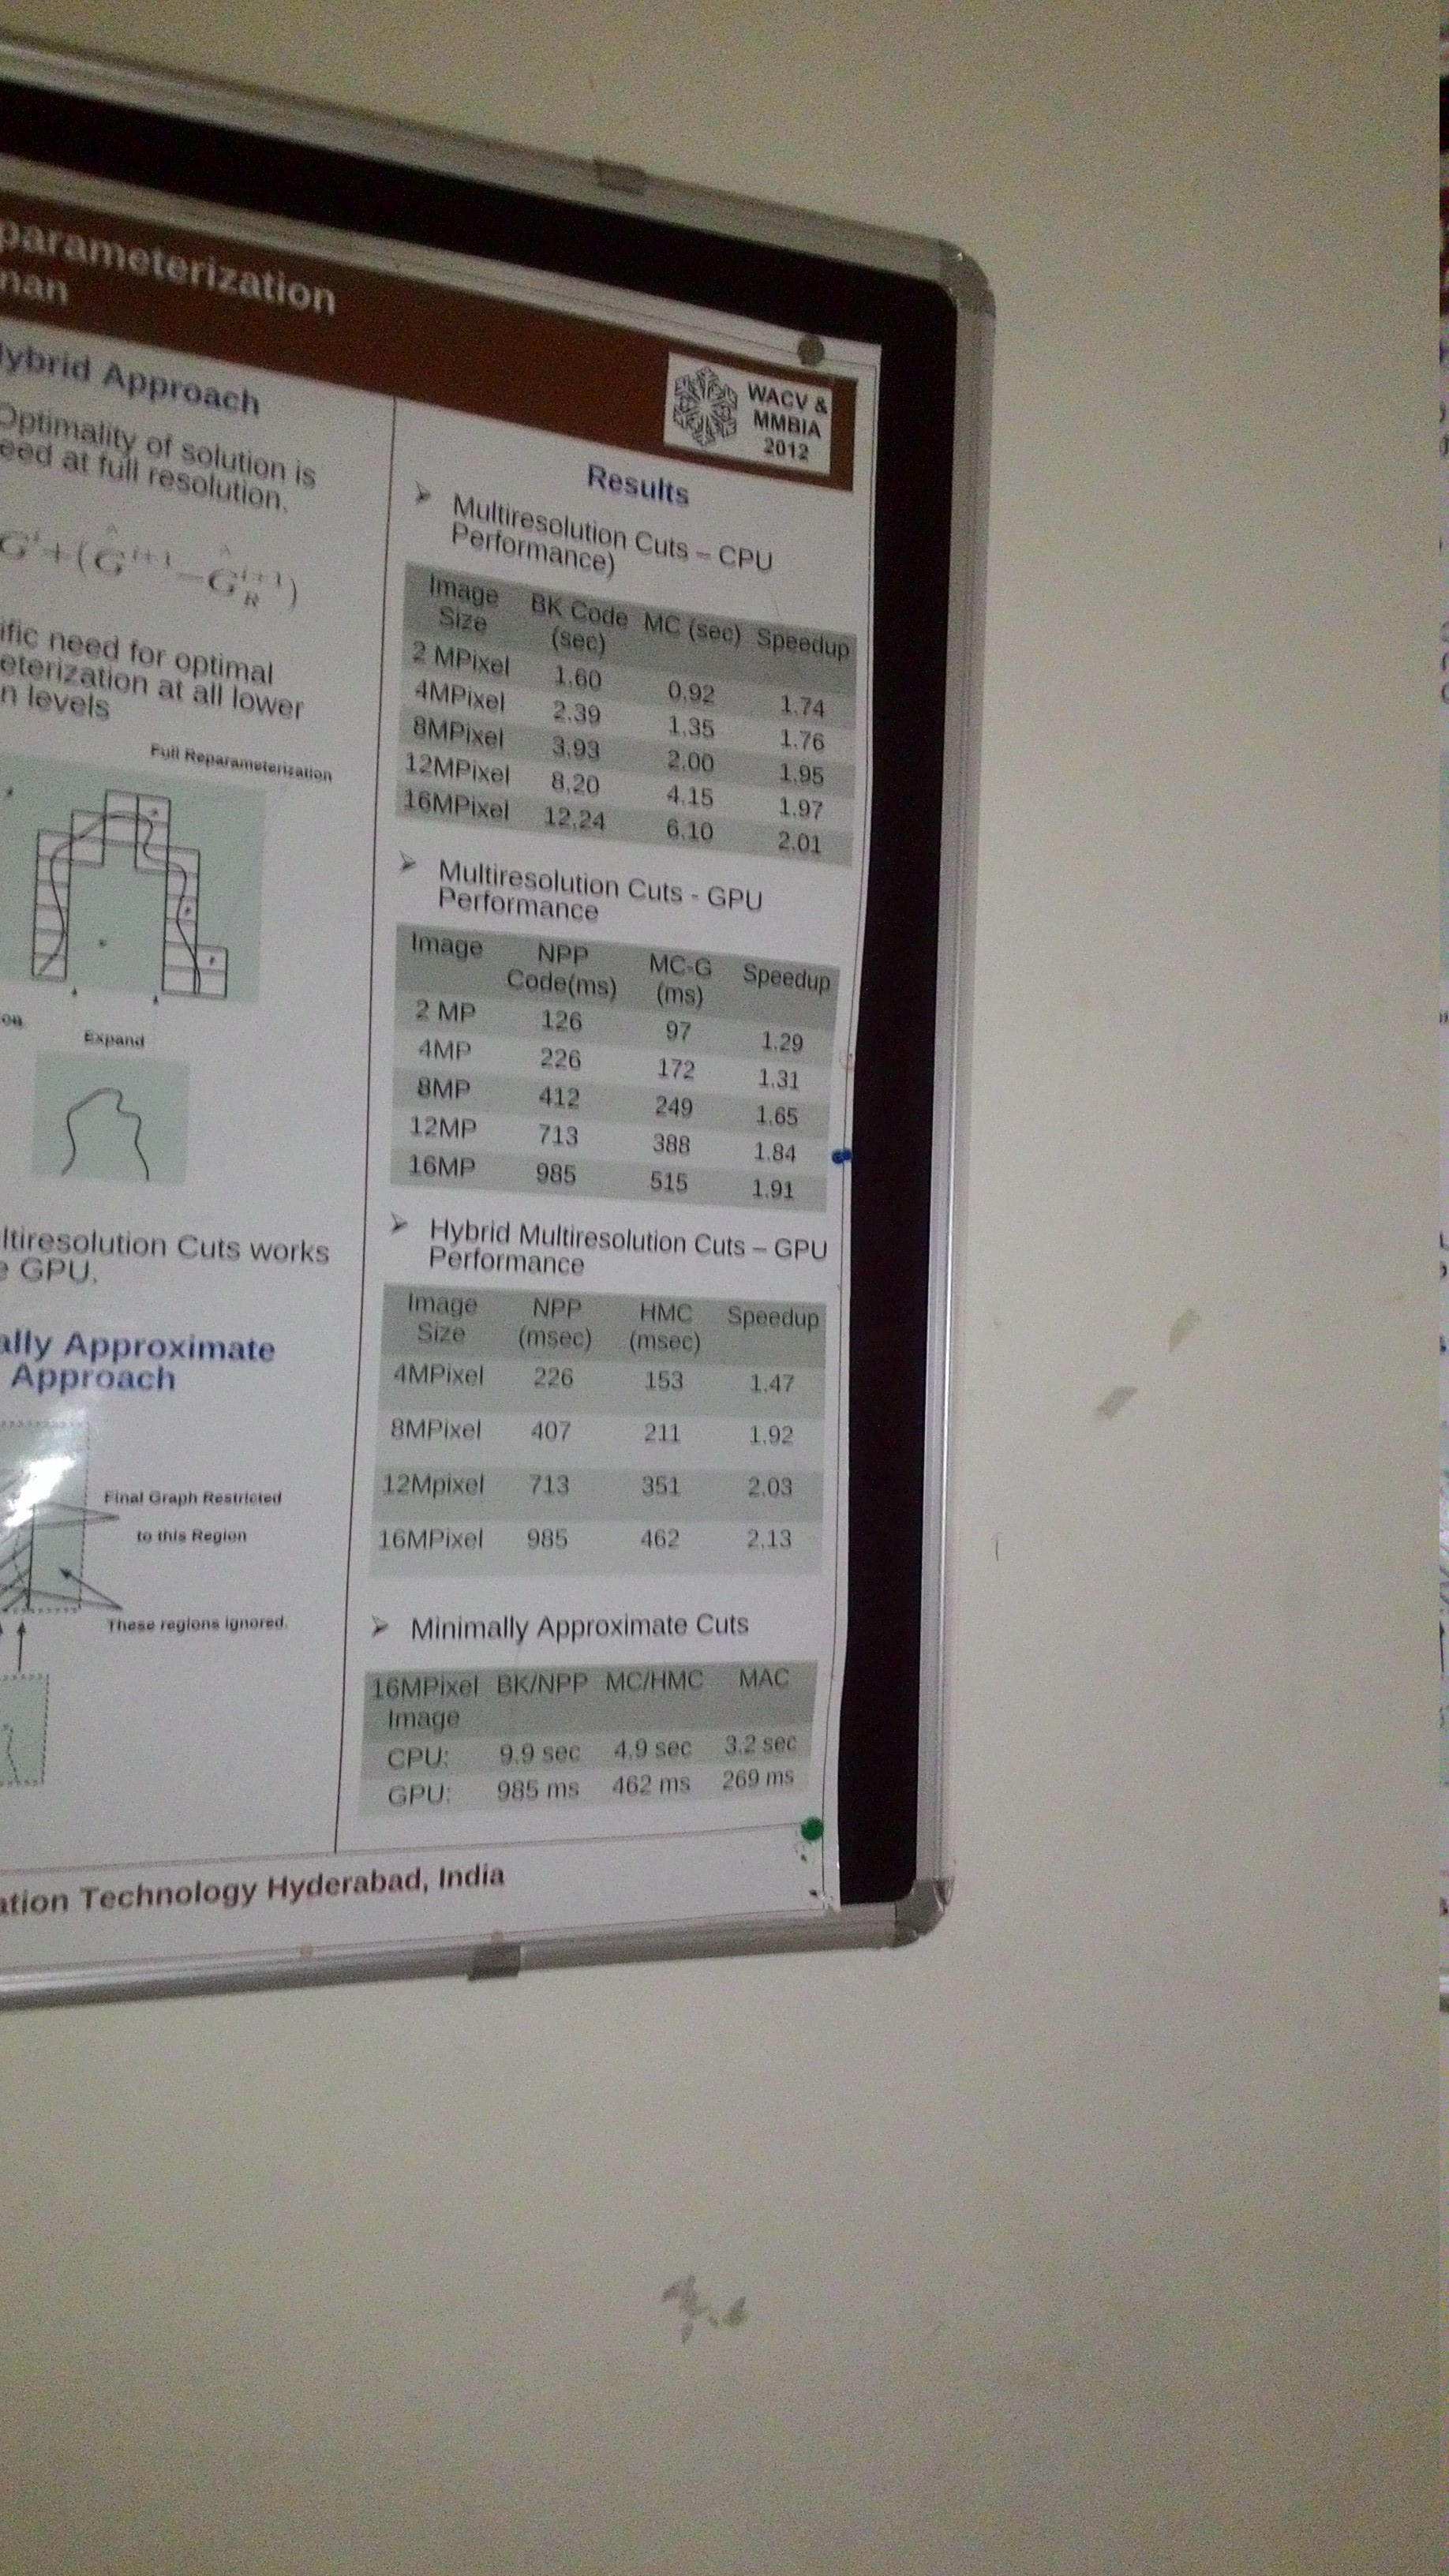
\includegraphics[width=0.3\textwidth]{planar3.jpg}\hfill
\caption{Planar Image 3}
\label{fig:Image 3}
\end{figure}

\vspace{20em}
\subsection{Output}

\begin{figure}[htp]
\centering
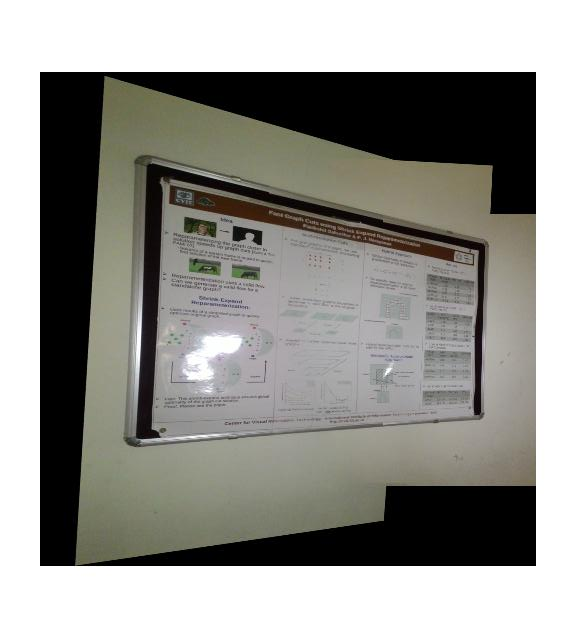
\includegraphics[width=0.7\textwidth]{planarstitch.jpg}\hfill
\end{figure}

\clearpage
\section{ Perspective Distortion Correction}
Perpective distortion is a warping or transformation of an object and its surrounding area that differs significantly from what the object would look like with a normal focal length, due to the relative scale of nearby and distant features. The perspective distortion of a planar surface can be understood as a projective transformation of a planar surface, which is a generalised linear transformation (Homography) in a homogeneous coordinate system
\subsection{Code}
The code for perspective distortion correction is as follows
\begin{lstlisting}
close all;
clear all;

Ia = imread('cal1.jpg');
Ib = imread('cal2.jpg');

imshow(Ia);
figure;
imshow(Ib);

p1 = [ 198, 407, 1;
    230, 1699, 1;
    2935, 1627,1;
    2915, 323, 1];

p2 = [270, 494, 1;
    502, 1279, 1;
    2355, 1315, 1;
    2607, 582, 1];
    
 p = dlt(p1, p2);
 p = p/p(3,3);
 T=maketform('projective',p');

[im2t,xdataim2t,ydataim2t]=imtransform(Ib,T);

xdataout=[min(1,xdataim2t(1)) max(size(Ia,2),xdataim2t(2))];
ydataout=[min(1,ydataim2t(1)) max(size(Ia,1),ydataim2t(2))];
im2t=imtransform(Ib,T,'XData',xdataout,
'YData',ydataout);
im1t=imtransform(Ia,maketform('affine',eye(3)),'XData',xdataout,
'YData',ydataout);

figure;
imshow(im2t);

\end{lstlisting}

\subsection{Input}
The input consists of 2 images, one taken at an angle from the plane and thus has perspective distortion; the other is taken from frontal and parallel view and thus having very less or no distortion. 

\begin{figure}[h]
\centering
\begin{minipage}{0.7\textwidth}
\centering
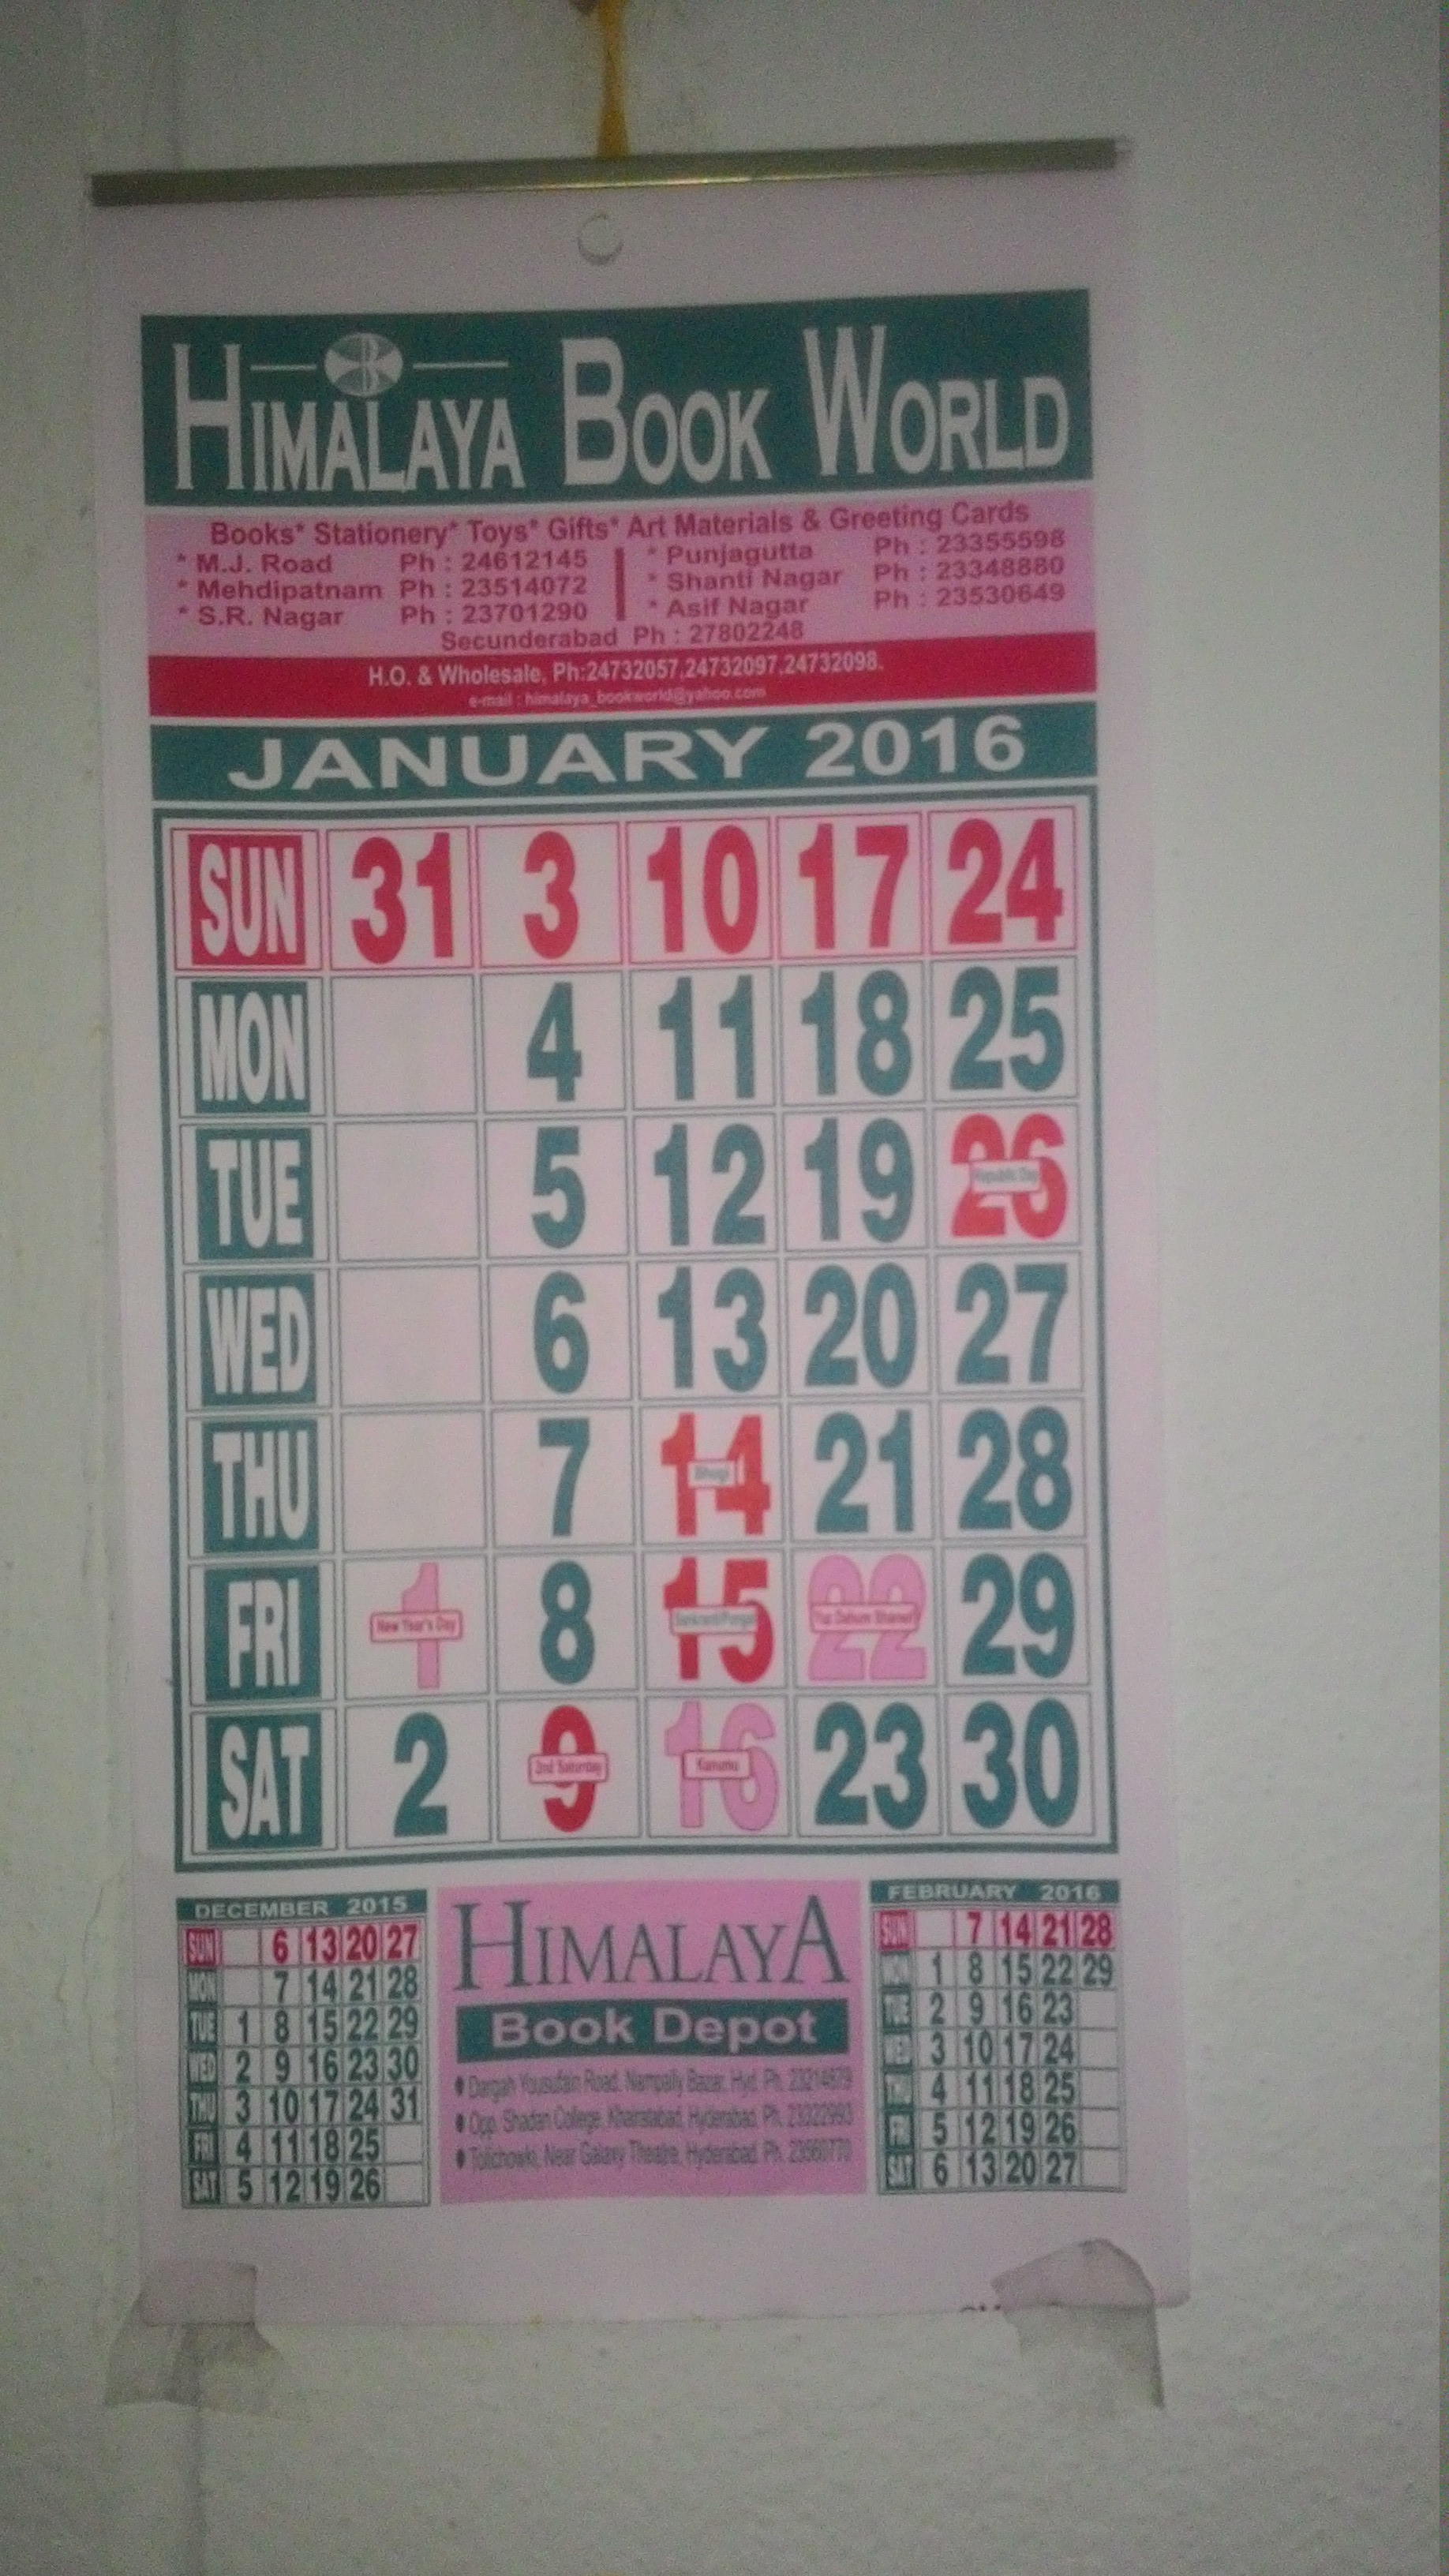
\includegraphics[scale = 0.07]{cal1.jpg}
\caption{Frontal View}
\label{fig:Image 1}
\end{minipage}%
\begin{minipage}{.5\textwidth}
\centering
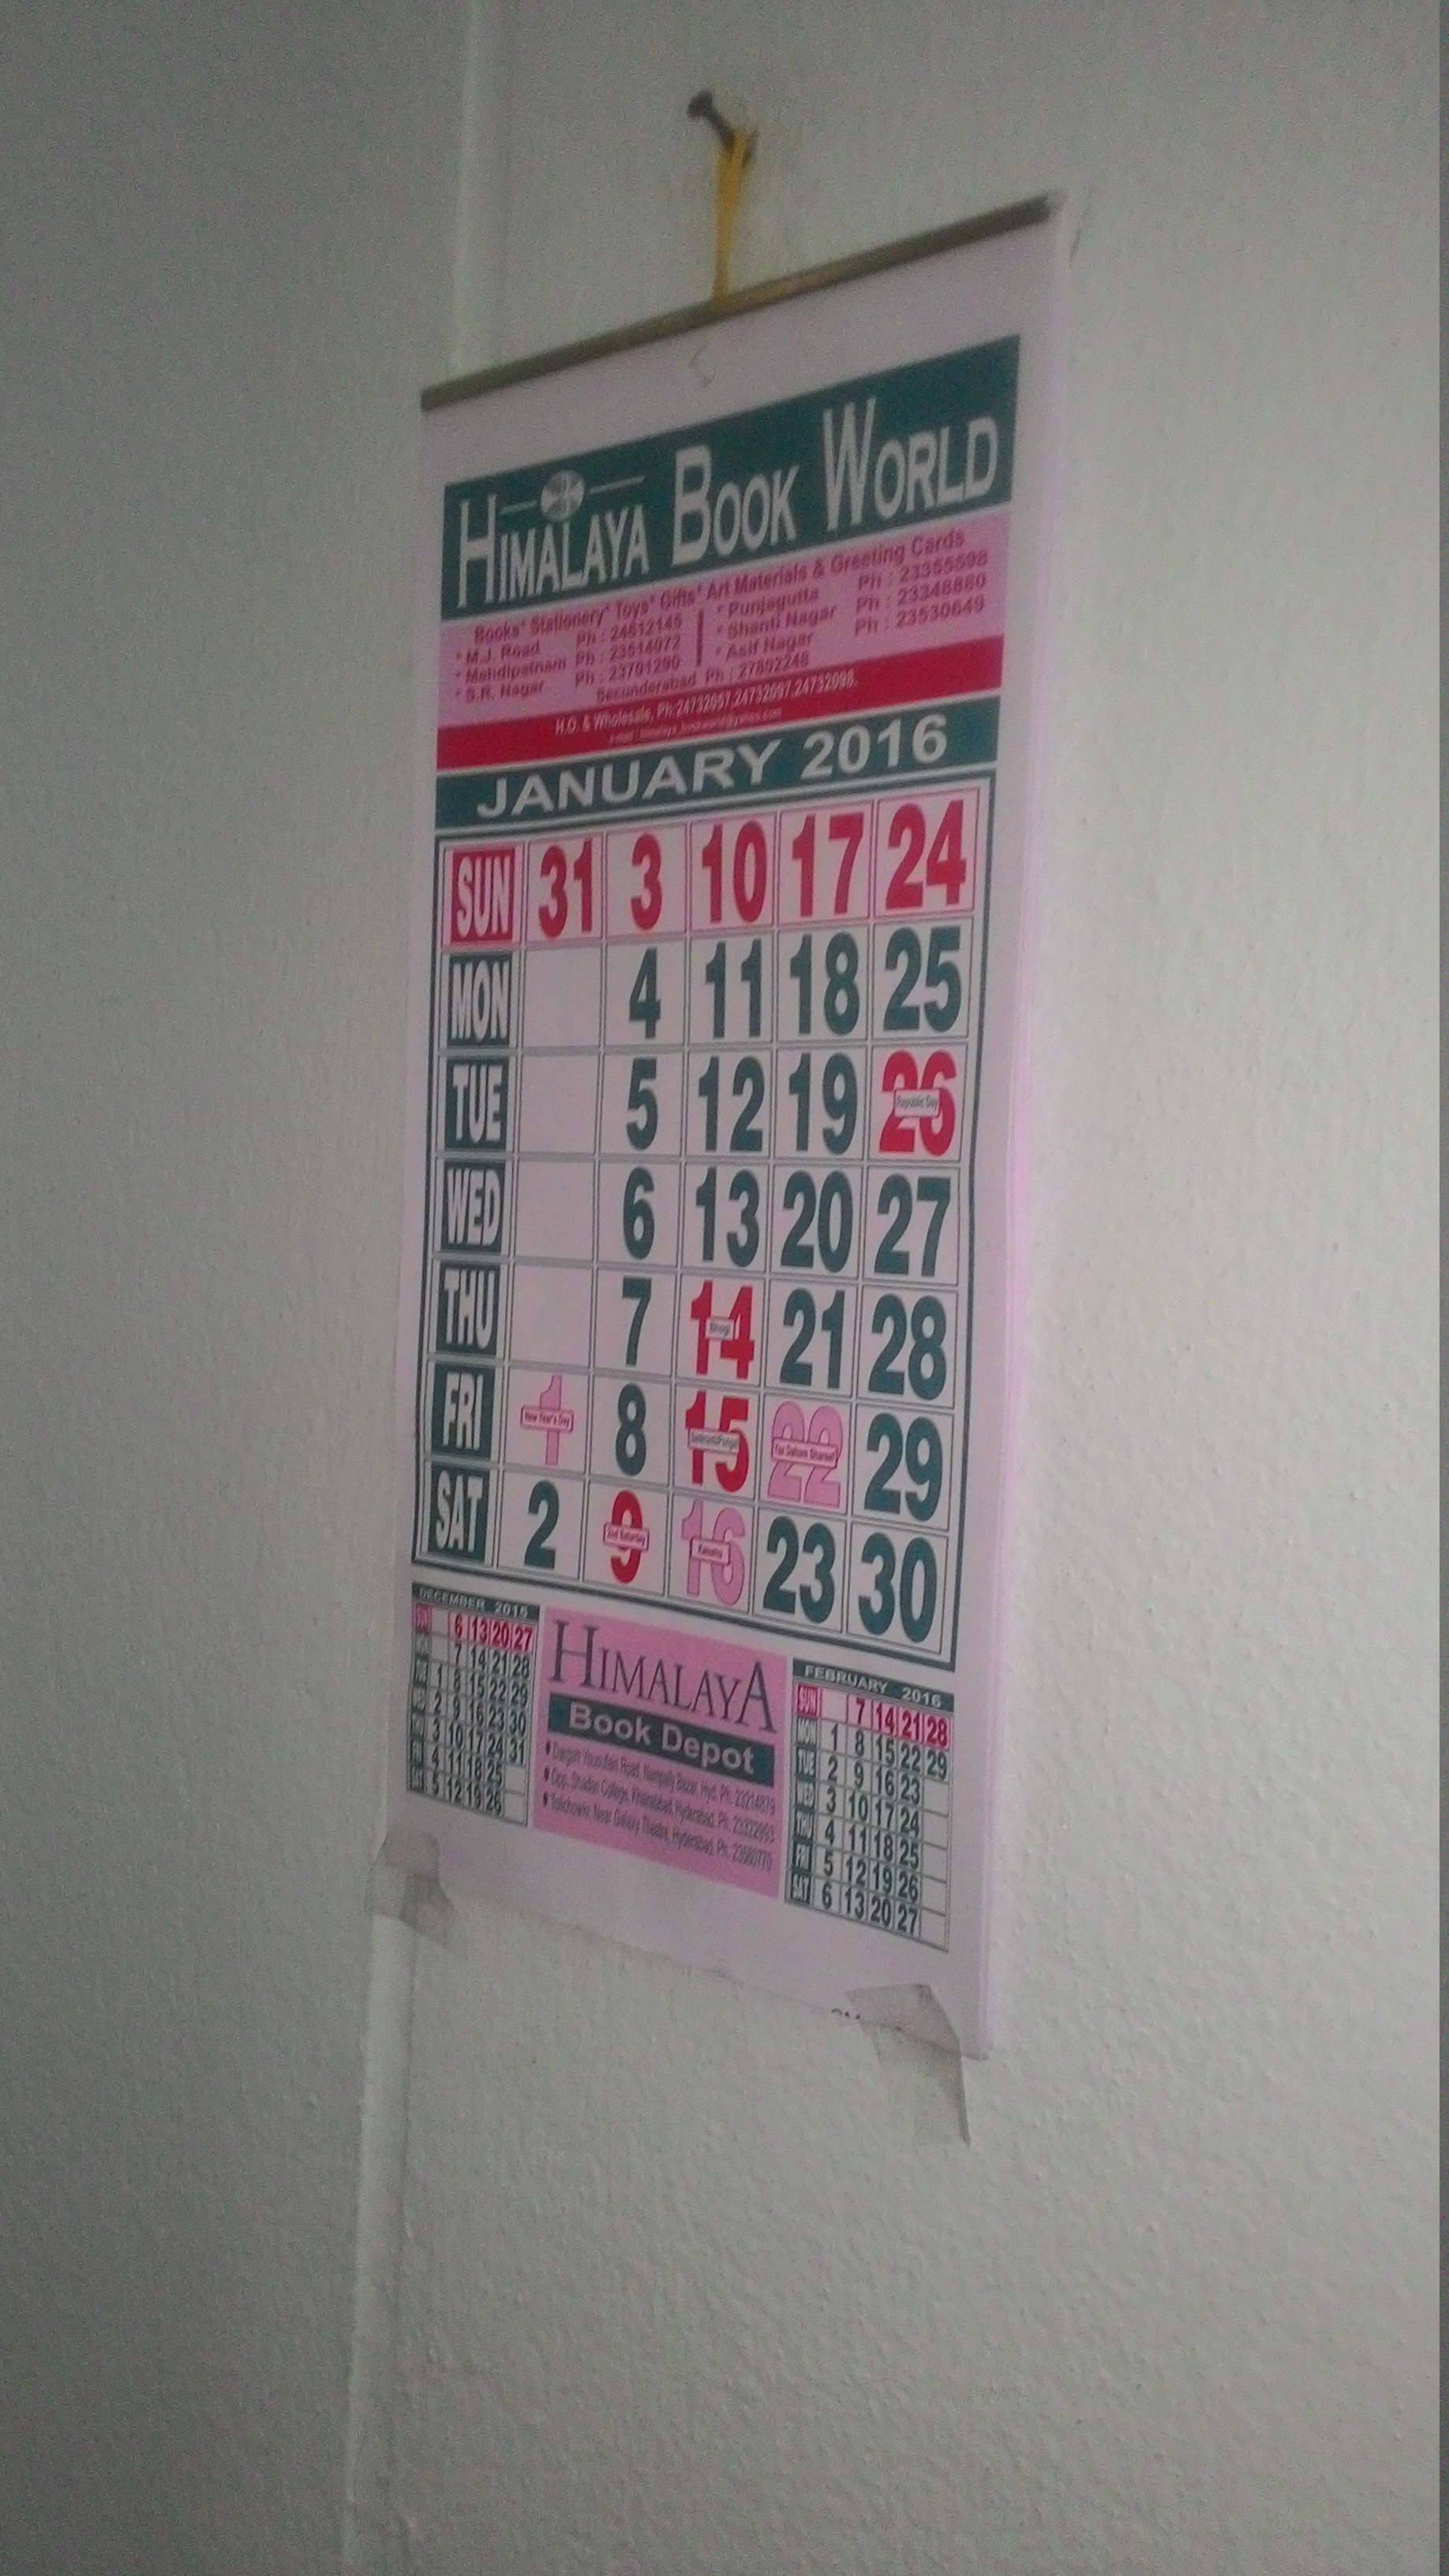
\includegraphics[scale = 0.07]{cal2.jpg}
\caption{Side View}
\label{fig:Image 2}
\end{minipage}%
\end{figure}

\subsection{Output}

\begin{figure}[htp]
\centering
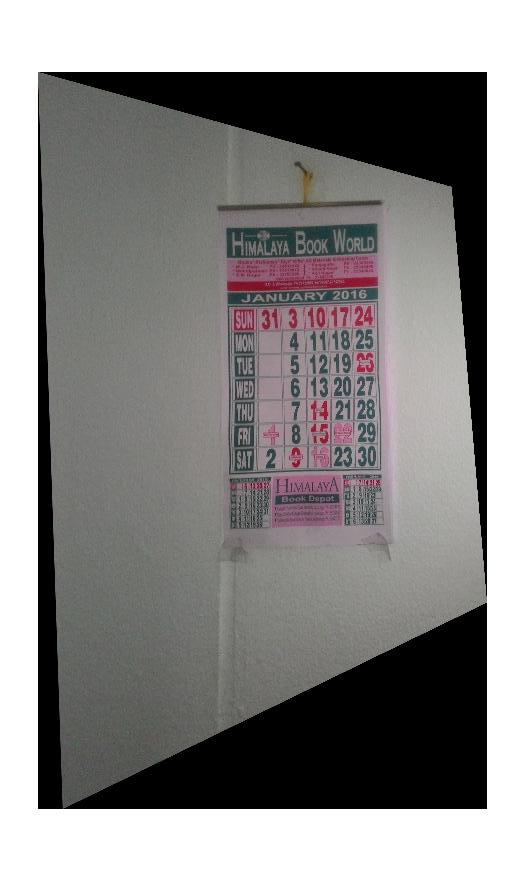
\includegraphics[width=0.6\textwidth]{distortionCorrect.jpg}\hfill
\caption{Undistorted Image}
\end{figure}

\clearpage
\section{Image Overlay}
\subsection{Code}
\begin{lstlisting}
function overlay()
    close all;
    clear all;
    Iaf = imread('field.jpg');
    Ias = imread('swimming.jpg');
    Iat = imread('tabletennis.jpg');
    Ib = imread('cocacola.jpg');

    p1Field = [530, 612, 1;
        658, 621, 1;
        720, 430, 1;
        657, 426, 1];

    p1Pool = [205, 320,1;
        254, 307, 1;
        169, 268,1;
        130, 276, 1];

    p1Table = [302, 118, 1;
        370, 120, 1;
        330, 206, 1;
        254, 200, 1];


    p2 = [1,1, 1;
        1, 117, 1;
        423, 117, 1;
        423, 1, 1];

    %% table

    p = dlt(p1Table, p2);
    p = p/p(3,3);

    [im1t, im2t]=transform(p, Iat, Ib);
    imsField = max(im1t,im2t);
    figure;
    imshow(imsField);


    %% pool
    
    p = dlt(p1Pool, p2);
    p = p/p(3,3);

    [im1t, im2t]=transform(p, Ias, Ib);
    %pool
    out = zeros(size(im1t));
    alphaR = 0.5;
    out(:,:,1) = alphaR * im1t(:,:,1) + (1 - alphaR) * im2t(:,:,1);
    alphaG = 0.5;
    out(:,:,2) = alphaG * im1t(:,:,2) + (1 - alphaG) * im2t(:,:,2);
    alphaB = 0.5;
    out(:,:,3) = alphaB * im1t(:,:,3) + (1 - alphaB) * im2t(:,:,3);
    imshow(mat2gray(out));


    %% field
    
    p = dlt(p1Field, p2);
    p = p/p(3,3);

    [im1t, im2t]=transform(p, Iaf, Ib);
    imsSwim=max(im1t,im2t);
    figure;
    imshow(imsSwim);


end

function [im1t, im2t] =  transform(p, Ia, Ib)
    T=maketform('projective',p');

    [im2t,xdataim2t,ydataim2t]=imtransform(Ib,T);
    
    xdataout=[min(1,xdataim2t(1)) max(size(Ia,2),xdataim2t(2))];
    ydataout=[min(1,ydataim2t(1)) max(size(Ia,1),ydataim2t(2))];
  
    im2t=imtransform(Ib,T,'XData',xdataout,
    'YData',ydataout);
    im1t=imtransform(Ia,maketform('affine',eye(3)),'XData',xdataout,
    'YData',ydataout);
   
    figure;
    imshow(im2t);
    figure;
    imshow(im1t);
    im2t = imresize(im2t, [size(im1t,1), size(im1t,2)]);

end

\end{lstlisting}

\subsection{Input}
To overlay image on images of sports images,  3 different images are used as show in figure

\begin{figure}[h]
\centering
\begin{minipage}{0.6\textwidth}
\centering
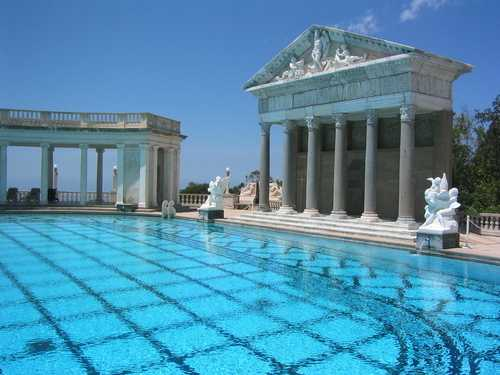
\includegraphics[scale = 0.45]{swimming.jpg}
\caption{Background Image 1}
\label{fig:Image 1}
\end{minipage}%
\begin{minipage}{.5\textwidth}
\centering
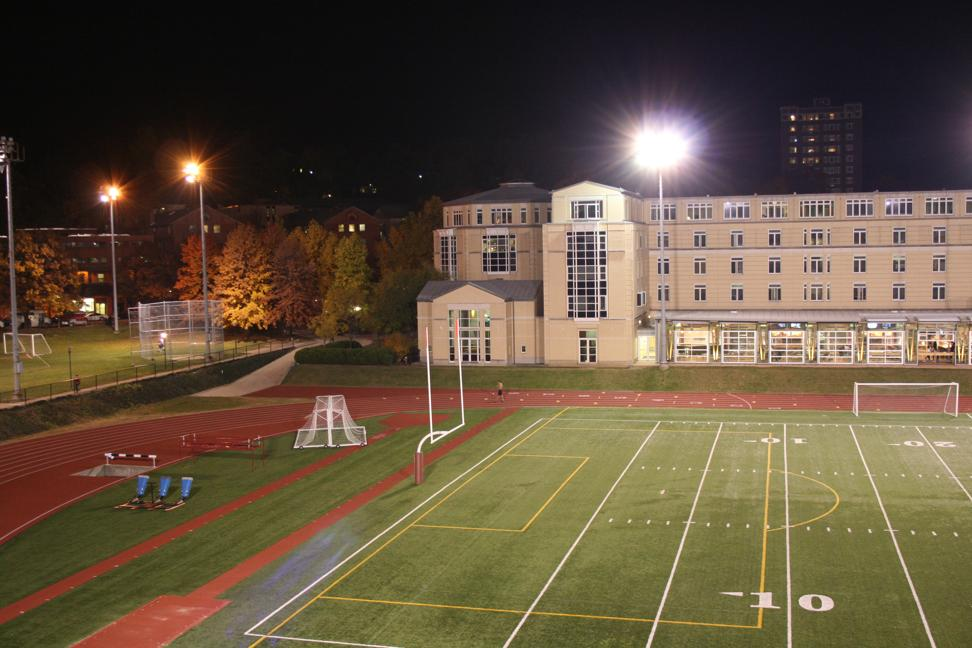
\includegraphics[scale = 0.25]{field.jpg}
\caption{Background Image 2}
\label{fig:Image 2}
\end{minipage}%
\end{figure}


\begin{figure}[h]
\centering
\begin{minipage}{0.6\textwidth}
\centering
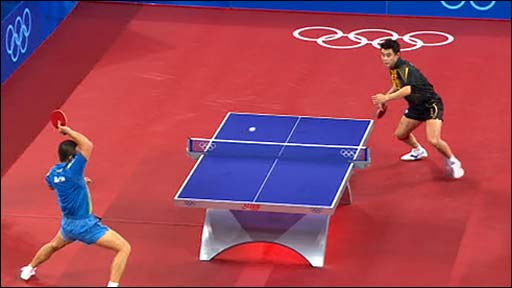
\includegraphics[scale = 0.45]{tabletennis.jpg}
\caption{Background Image 3}
\label{fig:Image 1}
\end{minipage}%
\begin{minipage}{.5\textwidth}
\centering

\includegraphics[scale = 0.45]{cocacola.jpg}
\caption{Overlayed Image}
\label{fig:Image 2}
\end{minipage}%
\end{figure}

\clearpage

   
\subsection{Output}
The following images were produced as output
\centering


\begin{figure}[htp]
\centering
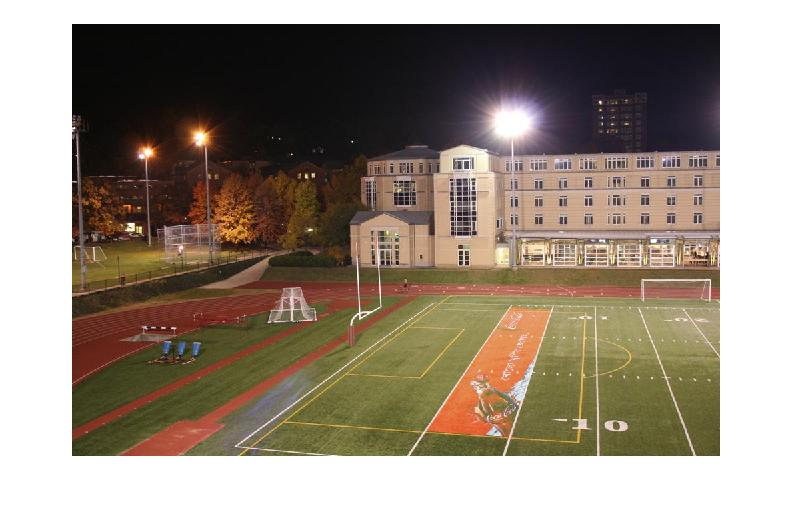
\includegraphics[width=1\textwidth]{overlayField.jpg}\hfill
\end{figure}

\begin{figure}[htp]
\centering
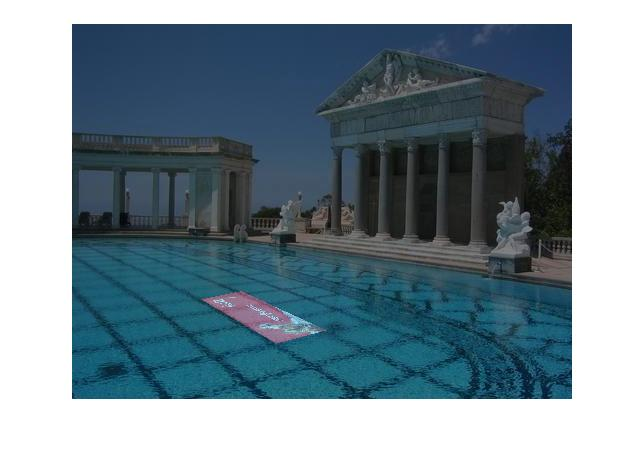
\includegraphics[width=1\textwidth]{overlayPool.jpg}\hfill
\end{figure}

\begin{figure}[htp]
\centering
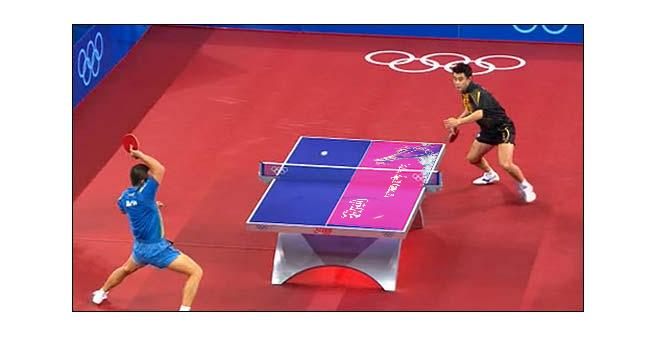
\includegraphics[width=1\textwidth]{overlayTable.jpg}\hfill
\end{figure}

\clearpage


\end{document}
